\documentclass[12pt, oneside]{book}
\pagestyle{headings}

\linespread{1.3}

\usepackage{geometry}
\geometry{a4paper}

\usepackage{graphicx}
\graphicspath{{img/}}
\usepackage{amssymb}
\usepackage{url}

\usepackage[table]{xcolor}
\usepackage{color, colortbl}

\usepackage[acronym]{glossaries}
\makeglossaries

\newacronym{sl}{SL}{Sri Lanka}
\newacronym{wp}{WP}{Western Province}
\newacronym{rpta}{RPTA}{Road Passenger Transport Authority}
\newacronym{ntc}{NTC}{National Transport Commission}
\newacronym{sltb}{SLTB}{Sri Lanka Transport Board}
\newacronym{dss}{DSS}{Decision Support System}
\newacronym{ict}{ICT}{Information and Communication Technology}
\newacronym{is}{IS}{information System}
\newacronym{gps}{GPS}{Global Positioning System}

\begin{document}


\title{
A Decision Support System
\\ for Public Transportation
\\ in Developing Countries
}
\author{Aftha Jaldin}
\date{\today}
\maketitle


\frontmatter

% begin Abstract
\clearpage
\chapter*{Abstract}

\paragraph{ } The Private Bus Passenger Transportation System is the most widely used Public Transportation System in Sri Lanka. It is used as the primary transport method for passengers within Colombo, the most populous city in the country, as well as between Colombo and other cities as well as suburbs.

However, the system is rife with inefficiencies and shortcomings. Delays, overcrowded buses and bus strikes are commonplace and the service is of poor quality. The problems in the system do not merely affect the transportation industry but has a knock-on effect to all walks of daily life for the people in the country. The productivity of the workforce suffers due to this inefficiency in the main public transport system.

The biggest problem that the commuters outline is the need to improve the service in terms of its schedule reliability and passenger overcrowding. Meanwhile, the bus operators complain that the revenue leakage is a major issue and needs to be rectified. However, the status quo continues without any solutions and these problems continue to haunt the average commuter.

Research into the issues as well as comments from frequent commuters has shown that the underlying cause is the lack of a proper Information System to assist the stakeholders in their decision making processes. Therefore, this research analyses the problems prevalent in the system and provides a solution to help minimize/eliminate the existing problems. The project identifies key aspects in the solution prototype and generalizes the results so that the concept can be applied to other developing countries with similar environments.


% begin Acknowledgement
\clearpage
\chapter*{Acknowledgement}
I would like to take this opportunity to thank the following people who have helped me thus far in my final year research project.
\begin{itemize}
\item Dr. Shiromi Arunatilake, for acting as my supervisor, overseeing my work and giving her valuable input into the thinking process of the project.
\item Dr. Jeewani Goonathilake, for providing her assistance whenever possible in her capacity as the Course Coordinator for the \acrshort{ict} Research Projects.
\item Mr. Pradeep Fernando, the Head of the \acrshort{gps} Tracking and Monitoring Unit of the \acrshort{ntc} for providing assistance in gathering information on the \acrshort{gps} tracking system which has been deployed on inter-provincial \acrshort{ntc} buses.
\item Mr. Dhanushka of the \acrshort{gps} Tracking and Monitoring Unit of the \acrshort{ntc} for providing information regarding the existing tracking system.
\item Mr. Muditha Navaratne from the Timetable Unit of the \acrshort{ntc}.
\item Dr. Chaminda Ranasinghe, Chief Executive Officer at IdeaHub (Pvt.) Ltd for providing his valuable insights.
\item Mr. K.A.R.A. Ranjith, the Operations Manager of the Western Province Passenger Transport Authority in providing information regarding the private bus service in the province.
\item Prof. Amal Kumarage, a Senior Lecturer of the Department of Transport and Logistics Management at the University of Moratuwa.
\item Mr. Janaka Weerawardana, doctoral student at the University of Moratuwa, Department of Transport and Logistics Management.
\item Mr. Anuradha Piyadasa, a Consultant and an Academic in the field of Public Transportation and Management.
\item Mr. Mahesh Nishan, Scheduling Officer at the \acrshort{wp} \acrshort{rpta}.
\item Mr. Theja Athukorala, Scheduling Officer at the \acrshort{wp} \acrshort{rpta}.
\item Mr. M. T. L. Cooray, Training Officer at the \acrshort{wp} \acrshort{rpta}.
\item To all the people who participated in the User Survey and helped me in my research.
\item and last, but certainly not least, my Parents for supporting me throughout the course of this research project.
\end{itemize}


\newpage

\pagenumbering{arabic}
\tableofcontents
\newpage

\pagenumbering{arabic}
\listoffigures
\newpage

\listoftables
\newpage

\printglossaries % prints just the list of acronyms
\newpage

\mainmatter

% begin Chapter Introduction

\chapter{Introduction}
\label{chapter-Introduction}

\paragraph{ } The Private Bus Transportation System is a famously contentious topic in Sri Lanka. For the average commuter, complaining about the system is part and parcel of everyday life. As a commuter myself and having used public transportation extensively for more than a decade, I have wondered many a time about the reasons why the bus service is in this state and why people keep complaining about it so very vehemently. The constant complaints are justified, as the bus service is grossly inefficient and lack proper service quality. The inefficiency in the system leads to lost productivity and dissatisfaction by the commuters. Eventually, it is the country that suffers from the lack of an efficient public transportation system for the people.

The initial objective of my project was to pinpoint the existing problems and possibly provide an IT solution for them. During the course of the research and interviews with the numerous people responsible, it occurred to me that the system has a myriad of things wrong with it. 

Careful management was the only requirement to overcome some problems, while others required a restructuring of the system, and still others required just an implementation of a solution and regulation of the service properly. Further research was required to identify underlying causes and provide a holistic solution to the problems. As I was passionate about the problem, I was intent on conducting a research to find solutions.

It is in this background that my research into the usage of a Decision Support System to solve problems in the local Public Transportation System was carried out. I did not immediately arrive at this solution, but gradually understood that the problems and the requirements of the stakeholders demanded such a system. Consequently, I attempted to identify and abstract the system's key components so that the over-arching concept can be applied to similar transportation systems in other developing countries.

\newpage

\section{Background Study: The Case of the \acrshort{wp} \acrshort{rpta}}
\label{section-BackgroundStudy}

\paragraph{ } Bus Passenger Transport is the highest and most widely used mode of public transport in Sri Lanka. The system is divided into Inter-Provincial and Intra-Provincial bus services. The service is operated by privately run (private buses) as well as state-run (SLTB) buses. The Sri Lanka Transport Board manages the SLTB buses and their jurisdiction is island wide regardless of the district or province. However, the organizational structure of private buses is different. All Inter-Provincial Private Buses are governed by the National Transport Commission (NTC) while the private bus services within each of Sri Lanka's provinces are governed by the Passenger Transport Authorities of the respective provinces. Accordingly, the Western Province Road Passenger Transport Authority (WP RPTA) handles the governance of the Private Bus Passenger Transport System in the Western Province. Please refer to Figure~\ref{image-busTransportSystemStructure} for an illustration of the Structure.

The major difference between the system in use in Sri Lanka and other countries is that the owners and operators of the buses are independent contractors and not the Central Government or the Provincial Authority. This has led to numerous problems and we shall discuss them in detail during the course of this document.

\begin {figure} [h!]
\centering
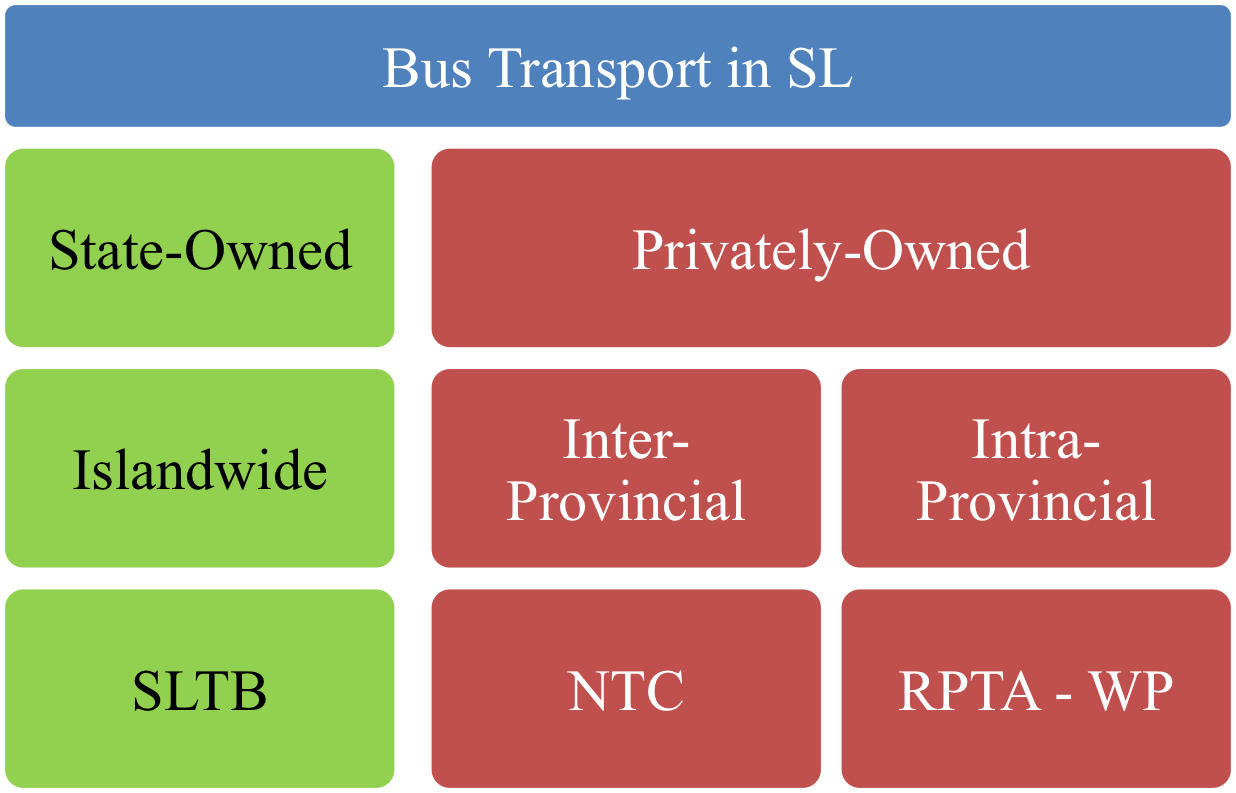
\includegraphics [scale=0.6] {busTransportSystemStructure}
\caption [Structure of the Bus Transport System in Sri Lanka] {The Structure of the Bus Transport System in Sri Lanka}
\label {image-busTransportSystemStructure}
\end {figure}

Let us take a look at the statistics involved with the bus service in Sri Lanka. According to the Draft National Policy on Transport in Sri Lanka \cite{MinistryofTransport2008}, public transport accounts for nearly 73\% of the total motorized passenger transport in the country. It also serves as the only means of transport for the majority of the population.

Of this, bus transportation accounts for nearly 68\% (a 93\% share in the public transport sphere), while rail transport accounts for the remaining 5\% (a 7\% share in the public transport sphere) \cite{MinistryofTransport2008}.

Within the bus transportation system, state-run bus services account for a 23\% share (about one-third of the share of bus transport) while private operators have a share of 45\% (a two-thirds share) provided by small-scale operators.

\begin {figure} [h!]
\centering
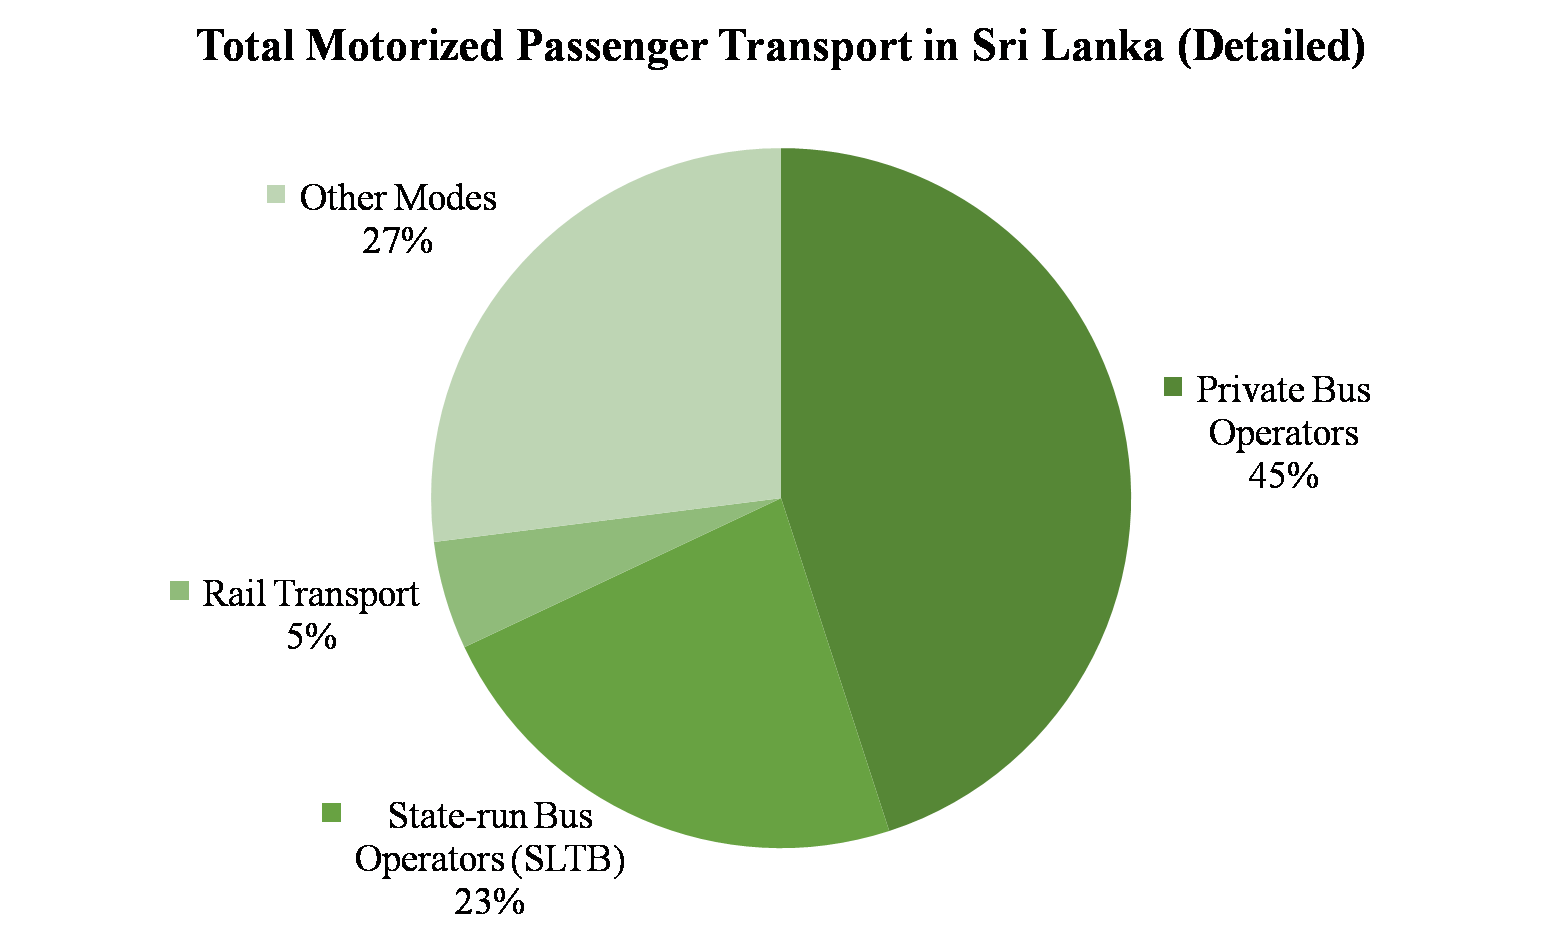
\includegraphics [scale=0.6] {totalMotorTransportPieChart}
\caption [Total Motorized Passenger Transport in SL] {Detailed View of Total Motorized Passenger Transport in Sri Lanka. Source: \cite{MinistryofTransport2008}}
\label {image-totalMotorTransportPieChart}
\end {figure}

Taking a look at the state-run bus service, data obtained from the Sri Lanka Transport Board show that approximately 2.5 million passengers island wide commute daily on close to 4500 \acrshort{sltb} buses \cite{SriLankaTransportBoard2010}. These buses travel an average of 2000km a day \cite{SriLankaTransportBoard2012}. 

Considering the buses operated by private bus operators, it is estimated that 10 million commuters travel daily on approximately 18,000 private buses currently in use in the country \cite{Silva2010}. Data gathered from the WP RPTA show that there are around 7000 private buses servicing the Western Province and its’ routes which is close to 450 in number. 

Looking at these statistics, we clearly see that the buses run by the private bus operators are far more in number compared to the state-run buses. It also shows that the majority of the commuters rely on the buses operated by private bus operators. These buses function as small independent operators and what is astounding is the fact that in 30 years of operation, not even a single major private bus operator has emerged. The private bus “cartel” is highly unionized and dictates terms to the commuters as well as the government on a regular basis \cite{AdaDerana2012}. Bus strikes are very common and when they do happen, the commuters are placed in great discomfort \cite{Samarajiva2012}, \cite{ColomboPage2012}.

In contrast, the state run bus service has a governing body, the SLTB, but it has been in steady decline since the 1970’s owing to mismanagement and cost overruns \cite{AnswersDotCom2012}. It has now become a money-sucking state entity and continues to waste the tax payer's money with no solution in the horizon \cite{LBO2011}, \cite{Sirimanne2013}. The number of SLTB buses in daily operation is well below the number of private buses and because of this, the state-run bus service is unreliable. Presently, it is but a teardrop in a sea of public transport dominated by the private bus operators. For example, as pointed out previously, there are more private buses in the western province (around 7000) than there are SLTB buses in the entire island (around 4500).Given that the average commuter cannot and does not wait for hours on end till an SLTB bus arrives, they have no other option but to use the private bus service. \cite{Wijayapala2012}, \cite{Azwer2012}

\subsection{Justification of Research Project}

\paragraph{} As mentioned earlier, the Private Bus service is the largest and most widely used Passenger Transport system not only in the Western Province but also in Sri Lanka. However, commuters are constantly dissatisfied with the service provided and there seems to be no alternative. The railway system has its own problems and inefficiencies and a solution to that demands separate research.

According to World Bank statistics, Sri Lanka’s population currently stands at 20.869 million people \cite{WorldBank2013}. Being the most densely populated, the Western Province has a population of 5.8 million people \cite{DepartmentofCensusandStatistics2012}, which is 27.8\% of the total population. This means that more than a quarter of the people in Sri Lanka live and commute in the Western Province. Therefore, it is clearly evident that an improvement in the level of service is needed seeing as it affects more than a quarter of the country’s population.

As mentioned previously, there are around 7000 private buses servicing the Western Province. To put that into perspective, the SLTB only has a cadre of 4500 buses islandwide. This means that there are more private buses in the Western Province than there are SLTB buses in the entire country. This shows that it is a large transportation system that affects more than a quarter of the population in the country on a daily basis.

Also of importance to note is that the number of complaints related to the Inter-Provincial Private Bus Service has doubled this year compared to last year. Chairman of the NTC is reported as saying that over 40 complaints are received per day and this number is increasing \cite{Wickremasekara2012}, \cite{Range2012}. This means that the current strategy of scheduling buses is clearly not working properly which is leading to increased commuter dissatisfaction and complaints.

Therefore, research into the private bus passenger transport system is essential. It is a large system that affects a large amount of people on a daily basis and the service needs to improve significantly in order for this country to be more productive, the people to be satisfied and for the country to be more attractive to tourists.

\newpage

\section{Existing Problems}
\label{section-ExistingProblems}
There are several issues that commuters highlight consistently. These are listed below. 
\begin {enumerate}
\item Loitering of buses at bus stops
\item Slowness of the buses
\item Unreliability of the bus schedule
\item Overcrowding of buses
\item Discourteous service by the bus operators (conductors as well as drivers)
\item Overcharging of bus fares (commuters complained mainly about not receiving the proper change money back from the conductor)
\item Cleanliness and general presentability of bus operators (conductors as well as drivers)
\item Lack of information (regarding the rules and regulations for the bus operators as well as the commuters, bus schedules, fare tables etc.)
\item Other issues pointed out consistently by commuters
	\begin {enumerate}
	\item Non-issuance of tickets
	\item Neglect of road rules
	\item Wreckless driving
	\item Diverting attention to other activities while driving (texting, talking on the phone, eating, drinking etc)
	\item Picking up and dropping off commuters at undesignated bus stops
	\item The operators (driver and conductor) don't wear the proper attire (the designated uniform)
	\item Failure to display the fare table to the commuters
	\item Operating without a valid driver's license, revenue license, and/or route permit
	\end {enumerate}
\end {enumerate}
References: \cite{Wickremasekara2012, Range2012}, comments by frequent commuters, data gathered through the Pilot Route Survey.

\newpage

\section{Reasons for the Problems}
Each of the above mentioned problems have reasons that may cause them. Let us take a look at some possible reasons.
\begin {enumerate}
\item Loitering, slowness and unreliability of the buses. (Points 1,2 and 3 above)
\begin {itemize}
\item These are mainly caused by bus operators failing to follow the proper timetable.
\item The time table itself could be at fault as it may allow the bus driver to go at a snail’s pace and be tardy.
\item The traffic situation in urban roads is also to blame for these 2 problems.
\item Delays are also caused by the lack of buses in a particular route. Again, this boils down to the inefficiency and ineffectiveness of the timetable.
\end {itemize}
\item Overcrowding of buses (Point 4 above)
\begin {itemize}
\item On one hand the bus operators are at fault for trying to maximize their profits by overcrowding the buses and disregarding passenger comfort and safety. On the other, the commuters are at fault for getting into an already crowded bus. The commuters feel that if they do not get into the bus right now, they might be late to their destination by waiting for another to come along. This may be caused by a lack of trust in the bus schedule so in effect this problem is caused by the timetables once again as pointed out previously.
\item It is important to note that the authorities allow this overcrowding to happen as they have no rules governing the crowds in buses.
\end {itemize}
\item Discourteous service, overcharging of bus fares and cleanliness \& general presentability of bus operators (Points 5, 6 and 7 above)
\begin {itemize}
\item The commuters frequently complain about these 3 points and the bus operators are solely to blame. They are a result of improper training and a lack of respect and professionalism in the industry.
\end {itemize}
\item Lack of information (Point 8 above)
\begin {itemize}
\item The blame for this lies with the bus operators as well as the regulatory body, the Western Province Road Passenger Transport Authority. The WP RPTA does not have a proper channel (website, information booklet etc.) to display and disseminate information regarding bus timetables and the rules and regulations governing the bus services etc. It is compulsory and of the utmost importance that this and other information is displayed to the pubic freely but it is not being done properly leading to the public frequently complaining and being misinformed.
\end {itemize}
\end {enumerate}

\newpage

\section{Current Bus Scheduling Process in Sri Lanka}
\label{section-CurrentBusSchedulingProcessInSriLanka}

\paragraph{ } Bus scheduling and timetabling in Sri Lanka (both inter and intra-provincial) has been a manual process in the past and it continues to be in the present day. Although IT tools can be used for scheduling and timetabling, the authorities still use an age-old manual process of scheduling buses for the bus routes (Data gathered through interviews with the Scheduling Unit of the WP RPTA).

Up until the mid 2000’s, the bus routes in the Western Province did not have proper bus schedules. The buses were dispatched from the terminals in the order and frequency they arrived. No scientific methodology was used in identifying headways, slack times or schedules. However, following the research efforts from the University of Moratuwa and Mr. Anuradha Piyadasa in particular, bus schedules were implemented, circa 2005. The methodology used in formulating these schedules is explored later in this section. These schedules were then agreed upon and put into circulation in the Western Province bus routes. Although, the formulation of these schedules was done using a software system (developed by Mr. Piyadasa), this system is not being used at the moment. The main steps of the process are illustrated in Figure~\ref{image-currentBusSchedulingProcess}.

\begin{figure}[h!]
\centering
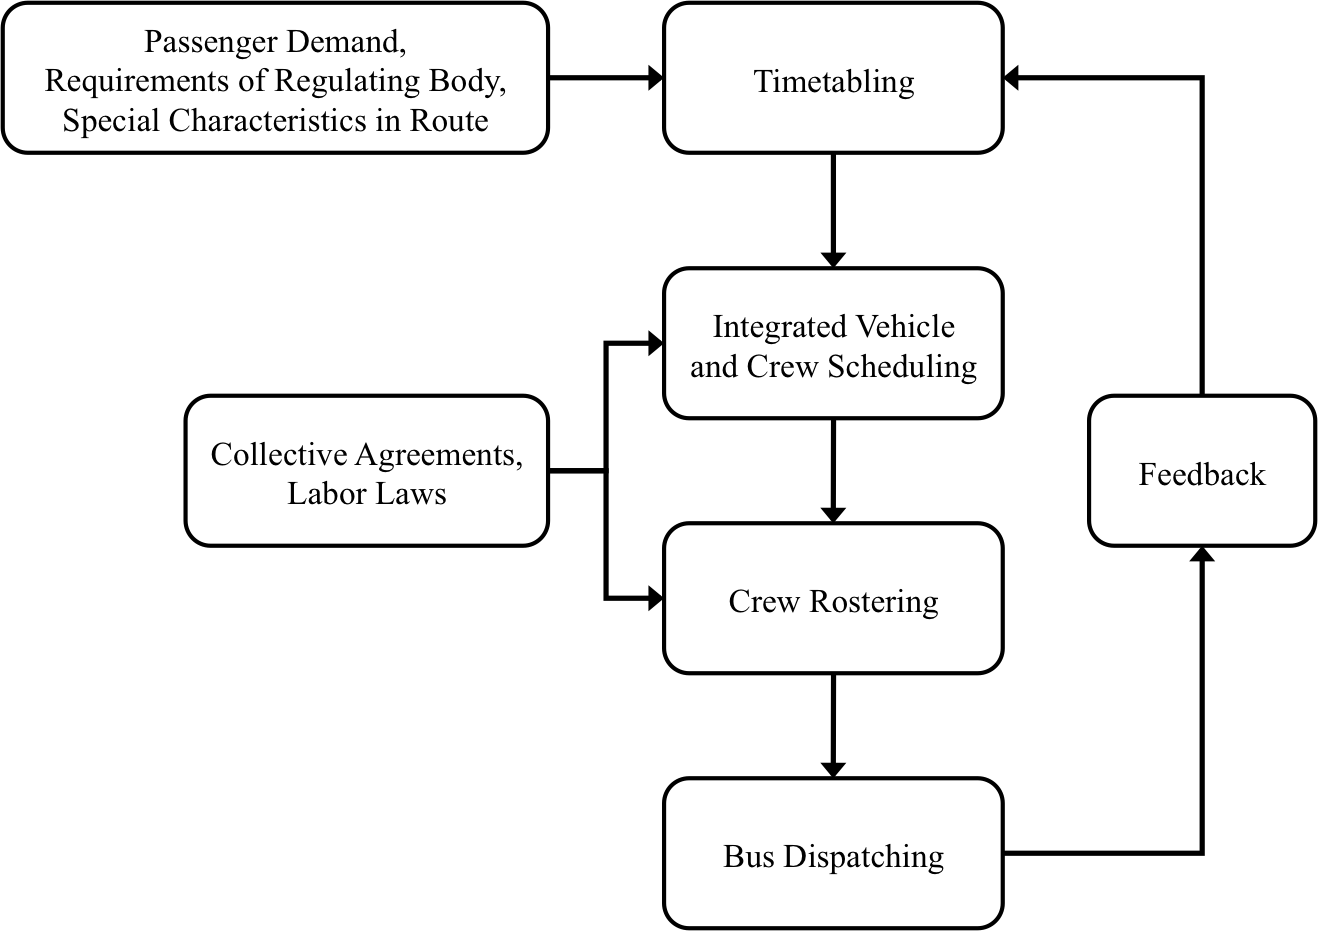
\includegraphics [scale=0.7] {currentBusSchedulingProcess}
\caption[Current Bus Scheduling Process in SL]{Current Bus Scheduling Process in Sri Lanka. Source: \cite{Piyadasa2005}}
\label{image-currentBusSchedulingProcess}
\end{figure}

This process of bus scheduling is an extension of the process put forth by Dennis Huisman in 2004 \cite{Piyadasa2005}. The first step of the process is to conduct a survey. This identifies the existing passenger demand, the quality of the service the buses provide on a given route, the requirements of the regulatory body and any special characteristics of a given route. 

The surveyors ride the buses at variously chosen days and times (to and from the main terminal), note down the trip times and identify the delays and loitering points of the buses on the given route. They also gauge the passenger demand by noting how crowded the bus gets at different stages of the trip. This is a rough estimate of the demand, as the surveyors do not have access to the exact quantitative data.

The next step is the timetable. They formulate this by calculating the average headway for the route. During the formulation of the timetable, the schedulers determine the time the bus service commences and terminates daily for the route. This is done through analyzing the passenger demand data they gather. It is important to correctly identify the time the service commences and terminates daily as it affects the revenue gained by the bus operators and may lead to the operators being unhappy with the timetable. If the service starts too early in the morning or ends too late at night the operators will run at a loss and will not be able to provide a proper service.

Next is the scheduling of the buses to the timetable. The scheduling officers schedule the buses to the bus routes manually using their observations, experience and knowledge. Once the scheduling is complete, the crew rosters are formulated using the schedules. 

Finally, the revised schedule is placed into circulation and used on the bus route (Source: Data gathered through interviews with the Scheduling Unit of the WP RPTA).

As the crew of a particular bus only operates that bus, the steps of vehicle scheduling and crew scheduling could be and should be carried out together. This is known as Integrated Vehicle and Crew Scheduling and literature to support this has been mentioned in the Literature Review of this thesis document.

As mentioned previously, until the mid-2000’s the private buses in the Western Province did not have predefined schedules to operate with. The buses were dispatched as soon as they came in to the terminal and the operators did not have predefined working hours and trips to complete for each working day \cite{Piyadasa2005}. However, thanks to research efforts by the University of Moratuwa almost all of the 450+ routes in the Western Province now have working timetables. Despite these timetables being implemented and in operation, they are not being properly adhered to and the quality of the bus service is still well below what is needed.

The bus schedules that are currently in operation take into account both the Economic and Financial cost of the service to the country, the commuters and the bus operators and optimizes the dispatching of the buses via optimal headway manipulation \cite{Piyadasa2005}. After doing numerous mathematical calculations, the methodology identifies the optimal average headway for the route. After identifying the headway, the available buses are scheduled to fill up the timetable as optimally as possible.

A software system was developed to be used to calculate the headways. Ironically however, the system is not being used by the WP RPTA to which it was developed. Instead they use a manual method of determining headway. The NTC however, uses the system to schedule the inter-provincial bus system (data gathered through interviews with Mr. Anuradha Piyadasa, the researcher and developer of the software system).

On inquiry from the personnel at the Scheduling Unit of the WP RPTA, they said that a common observation was that there is a plethora of buses for many of the bus routes in the province, which leads to scheduling difficulties for the Authority. This is due to previous regimes simply doing surveys on the bus service and adding additional buses to the roads, regardless of the requirement. Bus route permits have been issued in mass numbers as a stop-gap solution to the ailing bus service without accounting for the effect it will have on the system as well as the traffic situation. This leads to the revenue gained by each individual bus gradually decreasing (The number of passengers aka the demand stays fairly constant while the number of buses increases which means there are more buses to share in the same revenue. This means that the revenue gained by each individual bus decreases). This has and continues to hinder any efforts for proper reform, restructuring and reengineering of the private bus service in the country.

The timetables that have been implemented currently have research backing them but the bus operators have found numerous ways to circumvent the objectives of these schedules which is to ensure a timely and efficient bus service. This became clearly evident during discussions with the Scheduling Unit of the WP RPTA and from the constant dissatisfaction by the commuters. The bus operators consistently look to maximize their profits with a disregard for the level of service offered to the passenger. The timekeepers and Officers-In-Charge at bus terminals also add to the problem by accepting bribes and neglecting their duties.

Obvious solutions to these problems would be to reduce the trip times in the schedules even more and implement tougher regulations. However, trip times can only be reduced up to a certain point before they become impracticable. The Scheduling Unit is revising the schedules at the moment but it is moving at a snail’s pace, not unlike the buses they schedule. 

Also of note is how the revision process is handled. A revision to an existing schedule is not done unless and until sufficient complaints are received from the commuters. One would then think that there was a reasonably efficient complaint process and system in place but this is not so. The complaint mechanism is non-structured which leads to a perfect storm of problems. The commuters are not made aware of the complaint mechanism (no proper channel of disseminating information to the public by way of website/mobile app etc) and complaints are not received, documented and acted upon in a proper fashion (At times only the security guard at the scheduling unit is available to answer the phone and take down complaints when they are received) leading to the status quo continuing. (Source: Discussions with the Scheduling Personnel at the WP RPTA)

\newpage


\section{Decision Support Systems: an Introduction}
\label{section-DSSIntro}

\paragraph{} According to the nature of the problems currently in the Transportation Service, it is evident that some form of Information System is required to properly manage and monitor it. A Decision Support System seems to suit the need of the transportation service. Therefore, a brief introduction to the concept is provided herewith.

Decision Support Systems are defined as a set of related computer programs and the data required to assist with analysis and decision-making within an organization. The emphasis in DSSs are towards the assitance they provide for the decision-making process. Further details about the idea of DSSs are presented in Section~\ref{section-DSS}.

The requirements of the Transportation Service are such that it suits the offering that DSSs provide. A mechanism that aids the Schedulers in their timetabling process workflow while providing Commuters with the necessary information about the Transportation Service that helps them arrive at an informed decision is exactly what is required. Furthermore, the system's requirements go beyond a simple Management Information System or a Standalone software solution. 

According to \cite{Fedra2000}, in a real-world scenario, a typical decision-making process involves the following characteristics,

\begin {itemize}
\item Multiple actors
\item Conflicting objectives
\item Multiple criteria
\item Plural rationalities
\item Hidden agenda
\end {itemize}

These are consequently exactly what is prevalent in the current Transportation Service in Sri Lanka. \cite{Fedra2000} also presents the following components as included in a general DSS architecture.

\begin {itemize}
\item Information resources
\item The analytical engine
\item The user interface
\end {itemize}

Therefore, it is clear that a DSS is the most suitable Information Systems solution for this type of problem. Later on, in Section~\ref{section-Alternatives}, a more thorough justification will be provided for choosing this type of solution.

\newpage

\section{Research Goals \& Objectives}
\label{section-ResearchGoalsAndObjectives}

\paragraph{ } Of the problems mentioned in Section~\ref{section-ExistingProblems}, implementing a better bus schedule could solve the first 3. The problem of overcrowded buses could also logically be solved through implementing an effective and efficient timetable. Therefore, this research project focuses on finding a solution to these 4 issues as they are the main and most commonly brought up by the commuters.

We can identify the main goal of the research project as the identification of an Information Systems Solution that assists the Schedulers of the Transport Authority while also providing information to the Commuters to help their decision-making process. 

The Schedulers main business process is the formulation of timetables and schedules and thus addressing it is a core requirement. On the other hand, Commuters need to have Information about the Bus Transportation Service on demand so that they can decide which routes to take, which buses to avoid etc. These two parties also need to be connected in the process of Service Feedback so that the Schedulers are provided with an indication of the level of Service provided by the bus operators. This would lead to a more efficient passenger transport service and will improve commuter satisfaction and productivity.

\section{Research Scope \& Limitations}
\label{section-ResearchScope}

\paragraph{ } The research focuses on finding a DSS-like solution to solve the problems of timetabling, scheduling and inforamtion availability. Improving the Schedules and providing a method for commuters to give feedback is what the research project strives to achieve. By achieving this, the bus transport service is improved and made more efficient and reliable. 

The research analyzes how a DSS could be applied to the domain of public transportation in a developing nation. The project then attempted to evaluate the hypothesis by testing it on a group of users. Data was collected via a quantitative survey for the Commuters as well as a qualitative analysis for the Bus Schedulers in the Transport Authority.

The data gathering and automated data collection aspects of the schedulers business process is not within the scope of this research. This project assumes that the data is available already and its integrity and validity is intact.

The research also does not attempt to provide or test any hypothesis related to the application of an Expert System-like solution. The project will limit itself to understanding the IS requirements of the domain and attempting to provide a DSS-like solution to the existing problems.

\newpage

\section{Outline of Thesis}
\label{section-OutlineOfThesis}

Beyond this point, the thesis document will be structured as follows. Chapter~\ref{chapter-LitReview} will provide a comprehensive review of the literature regarding the planning process of a typical public transportation system. The Chapter also provides an overview of the literature related to Decision Support Systems and gives the reader a look at the concept of DSSs. The Section will also touch on the history and evolution of the DSS concept. The Chapter ends with a brief look at some Information Systems related to transportation services in a few other developing countries.

Chapter~\ref{chapter-ResearchMethodology} will discuss the research methodology followed in this project. It details the steps taken in the research process and identifies possible alternatives for the research problem. The Chapter will also provide information on a Pilot Route Survey that was conducted to gauge the requirements of the system and the shortcomings of the transportation service.

The details of the Proposed Solution will be provided in Chapter~\ref{chapter-ProposedSolution}. the Chapter will detail all the functionality as well as give the reader an overview of the entities in the proposed system. it will end by providing some UI screenshots of the prototype system.

Chapter~\ref{chapter-ResearchEvaluation} will detail the steps taken in the Evaluation phase of the research. the steps taken to evaluate the concept as well as the survey results will be noted in this chapter.

Finally in Chapter~\ref{chapter-ConclusionAndFutureWork}, the conclusions of this research project will be provided and possible future work will be discussed.

% begin Chapter LiteratureReview

\chapter {Literature Review}
\label{chapter-LitReview}

\paragraph{ } In the previous chapter, we discussed and analyzed the background and current state of the private bus service in the Western Province. An introduction to Decision Support Systems and how they relate to the transportation problem was also provided. The chapter also included a thorough explanation of the current bus scheduling process in the WP RPTA. We shall now take an in-depth look at the theoretical aspects of the planning process of public transportation, a more thorough analysis of Decision Support Systems and look into a few transportation systems in other countries.

\section{Planning Process of Public Transportation}

\paragraph{ } The planning and scheduling process of a public transport company generally comprises of 4 main steps, which are \textit{timetabling}, \textit{vehicle scheduling}, \textit{crew scheduling}, and \textit{crew rostering}. The transport mode could be a bus, tram, metro, train or airline. Figure~\ref{image-genericSchedulingProcess} illustrates the flow of the traditional scheduling process. It is carried out as is or the crew scheduling is carried out prior to the vehicle scheduling in certain instances. However, in recent times, the industry has begun adopting an integrated approach of carrying out the vehicle and crew scheduling together. This is also discussed later in the chapter \cite{Huisman2004}.

\begin {figure} [h!]
\centering
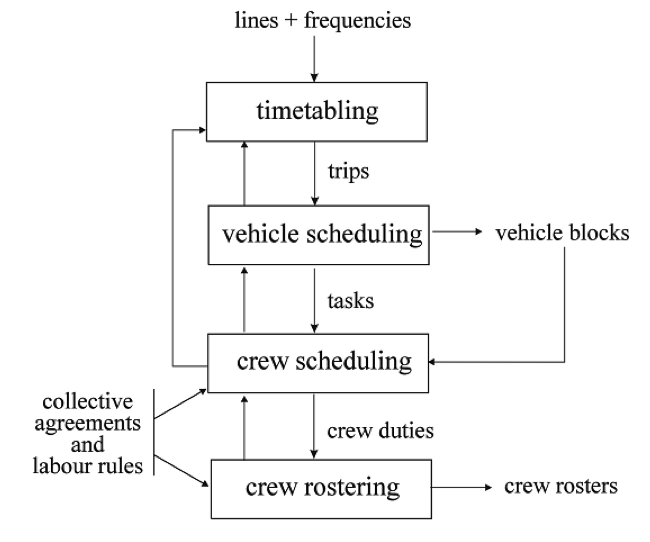
\includegraphics {genericSchedulingProcess}
\caption [Scheduling Process of a Public Transport Company] {Scheduling Process of a Public Transport Company. Source: \cite{Huisman2004}}
\label {image-genericSchedulingProcess}
\end {figure}

Decisions about which routes or lines to operate and how frequently, are inputs for the operational planning process. They can be either given by the marketing department of the company or determined by (local, regional or national) authorities. Furthermore, the travel times between various points on the route are assumed to be known. Based on the lines and frequencies, timetables are determined resulting in trips with corresponding start and end locations and times.

The second planning process is vehicle scheduling which consists of assigning vehicles to trips, resulting in a schedule for each vehicle. The vehicles, which are not in use for some time, are parked in a depot. A schedule for a vehicle is split into several vehicle blocks, where a new vehicle block starts at each departure from the depot. On such a block a sequence of tasks can be defined, where each task needs to be assigned to a working period for one crew (a duty) in the crew scheduling process. The feasibility of a duty is dependent on a set of collective agreements and labor rules that refer to sufficient rest time etcetera. Crew scheduling is short term crew planning (one day), i.e. assigning crew duties to tasks on each specific day, while the crew rostering process is long term crew planning (e.g. half a year) for constructing rosters from the crew duties.

\subsection{Timetabling}

\paragraph{ } Timetabling is the process of determining how frequently buses must operate on routes based on passenger demand and the operational plan of the respective authority and generating corresponding start and end locations and times of trips, based on these frequencies. Furthermore travel times between various points in routes, lengths of routes are assumed to be known \cite{Huisman2004}.

The main consideration in the process of timetabling is the output of headways, or the time between consecutive buses. Currently, average optimal headways are calculated in Sri Lanka and used in the scheduling process. An explanation of this process has been given in the previous chapter.

Let us take a look at previous research done into this area. \cite{Newell1971} provides the basic dispatching policy for a transportation route. This work has been the basis for many future work including \cite{Kumarage2007} research paper on formulating an optimal bus dispatching policy under variable demand over time and route length as is the case in Sri Lanka. The paper considered a method that was an extension to \cite{Newell1971}'s Optimal Dispatching Policy to determine a fleet size and dispatching rate based on both the operator's cost and user's cost including the disutility of standing, in order to arrive at a global cost optimum.

\cite{Riano2004} propose a stochastic model for Bus Dispatching that uses a linear programming model so that it is solvable easily and can be used for other modes of mass transit as well. A feature of this model is that it should be applied to modes of mass transit where the frequency is high enough so that users do not need to know the
schedule in advance (such as the one in Sri Lanka) The solution technique is based on a novel Transient Little Law.

Alternatively, \cite{Daganzo2008} describes an adaptive control scheme to mitigate the problem Bus Bunching in a Public Bus Transport system. This is a problem closely related to timetabling and scheduling and thus has been included in this Literature Review. Bus schedules cannot be easily maintained on busy lines with short headways. Experience shows that buses offering this type of service usually arrive irregularly at their stops, often in bunches. Although authorities build slack into their schedules to alleviate this problem, if necessary holding buses at control points to stay on schedule, their attempts often fail because practical amounts of slack cannot prevent large localized disruptions from spreading system-wide. 

The proposed scheme dynamically determines bus holding times at a route’s control points based on real-time headway information. The method requires less slack than the conventional, schedule-based approach to produce headways within a given tolerance. This allows buses to travel faster, reducing in-vehicle passenger delay and increasing bus productivity. One disadvantage of this method when thinking in terms of a Sri Lankan context is that it requires real-time information which cannot be obtained currently in the Bus Transport System in Colombo.

\cite{Xuan2011} look at the timetabling problem and its effect on schedule reliability a little differently. They study several Dynamic Holding Strategies that use the current state of all buses, as well as a virtual schedule. The virtual schedule is introduced whether the system is run with a 
published schedule or not. Through their research, it was found that through a dynamic holding strategy buses can both closely adhere to schedule and maintain regular headways without too much slack. This in turn improves Schedule Reliability and Commercial Speed of the buses.

\cite{Ceder2009} in his paper, put forth a methodology framework with developed algorithms for the derivation of vehicle departure times (timetable) with either even headways or even average passenger loads. The latter would be ideal for a situation like in Sri Lanka where overcrowding is a major complaint among the commuters.

\cite{Qian2013}, in their paper studied the Optimizing Mathematical Model of Bus Departure Interval and its Solution, and then worked out the best Bus Departure Interval (i.e.: the Headway). They established the optimizing mathematical model of bus departure interval, which took crowding cost of passengers into account, including passengers’ on-the-bus time cost, passengers’ crowding cost and bus company cost. The paper used a genetic algorithm to solve the problem. Reasonable bus departure intervals were obtained quickly by this method.

Furthermore, \cite{Fu2003} presented a new transit operating strategy in which service vehicles operate in pairs with the lead vehicle providing an all-stop local service and the following vehicle being allowed to skip some stops as an express service to address the bus dispatching and timetabling problem. The underlying scheduling problem is formulated as a nonlinear integer programming problem with the objective of minimizing the total costs for both operators and passengers. This could possibly be adapted into the Sri Lankan context as a viable alternative to the current scheduling methodology.

Finally, \cite{Sun2008} studied the headway optimization and scheduling combination of Bus Rapid Transit (BRT) vehicles. A model was proposed to minimize passengers' travel costs and vehicles' operation cost, and constraints included passenger volume, time, and frequency. The scheduling combination was composed by Normal, Zone, and Express scheduling. The model was solved by a genetic algorithm of variable-length coding. The result of the numerical case showed that the optimization results can save 69.92\% of the cost. A sensitivity analysis that was carried out showed that, under higher traffic volume or lower speed, the travel cost can be reduced through reasonable scheduling combination. The method was, therefore, proven scientifically and is feasible. A similar scheduling method of using Normal, Zone and Express Scheduling could possibly be implemented in Sri Lanka.

\subsection{Vehicle Scheduling}

\paragraph{ } Vehicle scheduling is defined as the process of assigning vehicles, to a set of predetermined trips, with fixed starting and ending times, while minimizing capital and operational costs. According to \cite{Freling2003}, the main objective of this step in the Scheduling Process is keeping the operational and capital costs of vehicles to a minimum.

The Vehicle Scheduling problem can be thought of through two perspectives. They are the Single-Depot Vehicle Scheduling Problem (SDVSP) and the Multiple-Depot Vehicle Scheduling Problem (MDVSP). As noticeable by their names, the difference is the number of depots that each Vehicle is assigned to. In the former, a given vehicle is assigned to a single depot while the latter situation assumes that a given vehicle is assigned to multiple depots. The SDVSP further assumes that all vehicles are identical and there are no time constraints \cite{Huisman2004}. Of these 2 approaches, only the SDVSP applies to the Sri Lankan context as each bus (and its crew) is issued a permit to ply on one route. Therefore, \cite{Freling2003} defines the Single-Depot Vehicle Scheduling Problem as follows.

“Given a depot at location \textit{d} and \textit{n} trips from locations \textit{b}$_i$ to \textit{e}$_i$, with corresponding fixed times \textit{bt}$_i$ and \textit{et}$_i$ (\textit{i}=1,...,\textit{n}),  and  given  the  travelling  times  between  all  pairs (\textit{d}, \textit{b}$_i$), (\textit{b}$_i$, \textit{e}$_i$), (\textit{e}$_i$, \textit{b}$_j$) and (\textit{e}$_i$, \textit{d}), find a feasible \textit{minimum cost} schedule for the vehicles, such that all trips are covered by a vehicle. Each trip has to be entirely serviced by one vehicle and trips serviced by the same vehicle are linked by \textit{deadheading trips} (\textit{dh}-trips).  These are trips without serving passengers (pairs (\textit{d}, \textit{b}$_i$), (\textit{e}$_i$, \textit{b}$_j$) and (\textit{e}$_i$, \textit{d})), consisting of travel time (vehicle deadheading) and/or \textit{idle time} (vehicle waiting time). A schedule for a vehicle is composed of vehicle \textit{blocks}, where each block is a departure from the depot, the service of a sequence of trips and the return to the depot. The cost function is a combination of vehicle capital (fixed) and/or operational (variable) cost. The capital cost is often such that the number of vehicles will be minimized, while the operational cost is often a combination of vehicle travel and idle time”.

In the Multiple-Depot Vehicle Scheduling Problem (MDVSP), buses are dispatched from several depots and total vehicles costs have to be minimized subject to the following constraints \cite{Huisman2004}

\begin {itemize}
\item Every vehicle is associated with a single depot; 
\item Every trip has to be assigned to exactly one vehicle; 
\item Some trips have to be assigned to vehicles from a certain subset of depots.
\end {itemize}

\subsection {Crew Scheduling}

\paragraph{ } The next step in the traditional scheduling process is the Crew Scheduling.  The problem is defined as follows: “The Crew Scheduling Problem (CSP) deals with assigning tasks to duties such that each task is performed; each duty is feasible with respect to a set of working rules and the total costs of the duties are minimized”. 

According to \cite{Huisman2004}, the only requirement with relation to the feasibility of a duty is its length or the working time in that duty, respectively. In most literature, the CSP is formulated as a set partitioning or covering problem and solved with a column generation approach.

\subsection {Integrated Vehicle and Crew Scheduling}

\paragraph{ } As mentioned previously in this chapter, the industry has begun using Integrated Vehicle and Crew Scheduling in recent times. This is due to logical as well as financial reasons. The airline industry uses this methodology as a crew has to be scheduled along with an airline trip for obvious reasons.

The Integrated Vehicle and Crew Scheduling Problem (Integrated VCSP or IVCSP) is analyzed by \cite{Huisman2004}. Accordingly, the Integrated Vehicle and Crew Scheduling Problem is defined as follows. “Given a set of service requirements or trips within a fixed planning horizon, find a minimum cost schedule for the vehicles and the crews, such that both the vehicle and the crew schedules are feasible and mutually compatible. Each trip has fixed starting and ending times, and the travelling times between all pairs of locations are known. A vehicle schedule is feasible if (1) each trip is assigned to a vehicle, and (2) each vehicle performs a feasible sequence of trips, where a sequence of trips is feasible if it is feasible for a vehicle to execute each pair of consecutive trips in the sequence”.

The author provides a very comprehensive look into the problem and presents a methodology to solve integrations of both the SDVSP and the MDVSP. The Integrated VCSP is also discussed by \cite{Freling2000} and \cite{Wren1997}.

\subsection {Crew Rostering}

The Crew Rostering Problem (CRP) aims at determining an optimal sequencing of a given set of duties into rosters satisfying operational constraints deriving from union contracts and company regulations. In the public bus transport industry, the roster is used to evenly distribute the workload among the crew \cite{Caprara1995}. Further studies were done by \cite{Kharraziha2003} and \cite{Tian2012}. The Integrated Crew Rostering Problem was examined in depth by \cite{Valdes2010} and \cite{Xie2012}.

This literature review looked at the different steps involved in the bus scheduling process. It also reviewed the literature related to each step. This literature is what will act as reference material as we attempt to present a new model of scheduling buses. The next chapter will detail the research methodology and the proposed model for scheduling buses in the Western Province.



\section{Automated Data Gathering}

\paragraph{ } While an automatic data gathering system would be immensely helpful to the scheduling unit of the WP RPTA, there is no such system in place currently. Such a system would aid in formulating proper timetables as well as monitoring and regulating the timetables and the buses for their adherence to said timetables. Proper and accurate data is very difficult to gather at the moment as all data gathering is done manually. This involves a huge amount of man-hours of work not forgetting the fact that the sample gathered is assumed to be representative of the whole system which might not always be the case.

Furthermore, a route survey is only done when there is a significant change needed to the timetable; otherwise the timetable is a fixed entity. This is a very reactive stance to the situation which is the incorrect policy to adopt as passenger demands vary and the service and the timetable needs to adjust accordingly. At present however, once the timetable is formulated and signed off by the higher authorities, it is not changed unless a significant number of people complain about. The service and timetable needs to be more proactive in order to offer a better service to the public (Source: Interviews with the WP RPTA and the NTC personnel).

An ideal Automatic Data Collection System (ADCS) would include provisions for Automatic Vehicle Location (AVL) data, Automatic Passenger Count (APC) data as well as the integration of an Automatic Fare Collection (AFC) System. Please refer to Figure~\ref{image-ADCS}. This would allow the schedulers to formulate much more accurate timetables taking into account the Passenger Demands (Load Factors) of the various buses at the various stops during various times of day. An Origin-Destination Matrix could also be obtained by analyzing this data to determine which segments of routes are most frequently used and therefore are more likely to be congested \cite{Wilson2008}.

\begin {figure} [h!]
\centering

\includegraphics[scale=0.6]{ADCS}
\caption [An Automatic Data Collection System] {An Automatic Data Collection System}
\label {image-ADCS}
\end {figure}

An implementation of an Automatic Data Collection System (ADCS) could ultimately lead to the creation of Dynamic Timetables. This means that the buses could be scheduled using real-time passenger demand data as well as traffic information and thus would better suit the commuters. However, the current system is to do the scheduling process manually in a strictly procedural fashion.

An ADCS has been proposed in the past but has been shot down and discouraged by the bus owners and operators. The main reason that they give for this is that the system is too costly for them to implement and it brings no additional value to them. This is a misguided notion by the owners and operators as the system could benefit them immensely in the long run. Revenue leakage, which is one of the main grievances given by bus owners, could be curbed through an implementation of an Automatic Fare Collection (AFC) System. Furthermore, it would bring about a sense of accountability and transparency in the payment of fares of private buses. It would be a cost in the short-term, but considering the long-term benefits, the owners/operators should consider it an investment to make the system and service future-proof.

Furthermore, an Automatic Vehicle Location (AVL) system would allow commuters to know exactly where and when the next bus will be arriving providing more information and flexibility. Automatic Passenger Counting (APC) would give the schedulers enough information to ensure that timetables are working correctly and buses are dispatched to account for higher or lower passenger demand. The schedulers could also audit their timetables more frequently to ensure that schedules are kept current. It would also allow route monitors to ascertain if the owners/operators are overcrowding the buses causing discomfort to passengers. An Automatic Fare Collection (AFC) system would also bring great comfort to commuters who consistently complain about being overcharged or not receiving the proper balance money back from the conductor. An AFC would also greatly benefit the owners/operators because they could monitor and audit their income correctly and put paid to the revenue leakage that occurs consistently (according to the owners) \cite{Wilson2008, Wilson2009, Wilson2012, Fijalkowski2010}.

\subsection{Automatic Data Collection in the Inter-Provincial Service} 

\paragraph{ } An Automatic Data Collection System is in place at the moment in the Inter-Provincial buses. The National Transport Commission (NTC) has taken steps to implement a system to track the location of the buses via a GPS tracking device fixed onto them. However, out of the 3500+ buses in operation in the Inter-Provincial service, only around 700 have been fixed with the device. Information obtained from the NTC states that a further 1000 buses will be equipped with the device within this year.

Currently, it only tracks the location and the speed of the bus. The system they have implemented consists of a device which is fixed on to the vehicle. This device tracks the location of the bus via GPS and relays the data back to the NTC servers via a GPRS connection. The device also contains an accelerometer to measure the speed of the vehicle. This allows the NTC to monitor the buses for possible speeding violations and reckless driving. Monitoring is done through a control center at the NTC head office in Narahenpita which is manned 24 hours a day. Apart from monitoring the buses, they provide information to the passengers and record complaints regarding errant bus operators.

Owners/operators can also choose to have a still camera fixed onto the bus as well. This is compulsory for Luxury buses and it allows the NTC monitor overcrowding of the buses. When a complaint is made to the NTC hotline, the personnel at the NTC control center can activate the camera and take a picture to decide if the bus is overcrowded or not. They can then instigate punishment proceedings for the bus involved.

The device costs around 45,000 rupees with the government subsidizing the cost. Eventually, the owners/operators have to pay only around 10,000 rupees. The objective of the NTC is to eventually have all the inter-provincial buses fitted with the device. This would allow the data to be collected automatically and that data would be used for the scheduling process and the formulation of timetables for the service (Source: Interviews with personnel at the NTC).

\subsection{Automatic Vehicle Location (AVL)}

\paragraph{ } Vehicle Location data could be obtained through several methods. One of the main and most feasible methods would be to fix a GPS-based tracker on to the bus and monitoring its movement through a mapping software. This method, however, has a fairly large startup cost which has discouraged the stakeholders in the past. Alternatively, this could be achieved by crowdsourcing the Vehicle Location data through a mobile app. Automatic Vehicle Location (AVL) Data is very important as it reflects the current location of a bus and can be used to predict journey times and availability of buses for the commuters. A system could be built that uses AVL data to notify commuters of the current bus, the bus that is due to arrive next etc. This data is also very important in the scheduling stage of transport planning and could be used to formulate more efficient and effective timetables \cite{Wilson2009}.

\subsection{Automatic Passenger Counting (APC)}

\paragraph{ } Automatic Passenger Counting (APC) is important in order to gauge the passenger demand or load factors in the buses. This data could be used to draw up origin-destination matrices in order to identify which segments of routes are most congested and which routes are not very congested at all. This all helps in the planning and dispatching of buses which eventually lead to a better schedule and a better service.

The APC data could be obtained from an Automated Fare Collection (AFC) System such as a contactless smart card payment method. The implementation of both could potentially be very useful for the commuters and owners/operators alike \cite{Wilson2009, Silva2010}.

\subsection{Automatic Fare Collection (AFC)}

\paragraph{ } The implementation of an Automatic Fare Collection system has been in the works for some time and discussions with industry experts have revealed that a working system is available. However it is not being implemented as the government still has some regulatory and other issues to sort out first. The system involves a Prepaid Smart Card system where the Smart Card could be used for cashless payment of bus fares. Commuters could also recharge their cards when the stored value in the cards runs low (akin to reloading a prepaid mobile phone). This is just one of the methods that could be used to implement an automated fare collection system \cite{Wilson2009, Silva2010}.

As its popularity grows, NFC or Near-Field Communication has garnered the attention of public transport systems around the world. It allows a user to use everyday devices (such as a mobile phone or an ATM card etc.) as a transaction medium. This could lead to enabling payment of bus fares with a mobile phone which is a very innovative and highly lucrative area to look into. It would bring comfort to passengers and allow owners/operators to receive the payment directly from the commuters. Therefore, the potential market and it's applications is vast. However, Sri Lanka does not have any such systems or parties interested in a system like this which is unfortunate. One could argue that before going to such technologically advanced lengths, the authorities should focus on a smaller system and implement one which is more appropriate to the Sri Lankan context which is a fair argument. The problem is that currently \textit{no system at all} exists, which is not a good situation for the private bus service and the country \cite{Silva2010, Sinha2012}.

As mentioned previously, the NTC has implemented a GPS-based Vehicle Tracking system in the Inter-Provincial Bus Transport Service as an Automated Data Collection System. However, it only collects the Vehicle Location data. The Passenger Counts data is not collected automatically and there is no system in place to do so. However, the Inter-Provincial Bus Service is more developed than the Intra-Provincial Service in the Western Province as the NTC has made it compulsory for Inter-Provincial buses to have Electronic Ticketing Machines (ETM). This means that at least the passenger counts data \textit{is} recorded. The data that is saved in the Ticketing Machines could be accessed later and the data be obtained for scheduling purposes.




\newpage

\section{Decision Support Systems}
\label {section-DSS}

\paragraph{ } Decision Support Systems are defined as a set of related computer programs and the data required to assist with analysis and decision-making within an organization. They are purposely developed to improve decision making of non-structured management problems. Decision Support Systems utilize data, provide an easy-to-use interface, and allow for the decision maker’s own insights hence being interactive, flexible, and adaptable computer-based information systems \cite{Turban2005}. 

Having said that, the term DSS in itself is difficult to define with academics and users differing in their opinion in terms of its preferred use. While academics have perceived DSS as a tool to support the decision making process, DSS users see DSS as a tool to facilitate organizational processes \cite{Keen1980}.

\subsection{History of Decision Support Systems}

\paragraph{ } The concept of a Decision Support System has been around since the 1950's but only recently has it increased in popularity and adoption in the industry. With the improvement in technology, the research into DSS's has also increased. The abstract concept of a system that aids in the decision-making process has its roots in the late 1950's and early 1960's through research done at the Carnegie Institute of Technology. This later grew into information systems research through work done at the Massachusettes Institute of Technology in the 1960's. DSS's started to become a research topic of its own in the mid-1970's with more and more research following through the mid to late 1980's \cite{Keen1980, Power2003}.

\cite{Power2003} lists 5 main categories of DSS's which are,

\begin {itemize}
\item \textbf{Communication-driven DSS} is a type of DSS that emphasizes communications, collaboration and shared decision-making support. A simple bulletin board or threaded email is the most elementary level of functionality. The comp.groupware FAQ defines groupware as "software and hardware for shared interactive environments" intended to support and augment group activity. Groupware is a subset of a broader concept called Collaborative Computing. Communications-Driven DSS enable two or more people to communicate with each other, share information and co-ordinate their activities. Group Decision Support Systems or GDSS is a hybrid type of DSS that allows multiple users to work collaboratively in groupwork using various software tools. Examples of group support tools are: audio conferencing, bulletin boards and web-conferencing, document sharing, electronic mail, computer supported face-to-face meeting software, and interactive video.; 
\item \textbf{Data-driven DSS} is a type of DSS that emphasizes access to and manipulation of a time-series of internal company data and sometimes external data. Simple file systems accessed by query and retrieval tools provide the most elementary level of functionality. Data warehouse systems that allow the manipulation of data by computerized tools tailored to a specific task and setting or by more general tools and operators provide additional functionality. Data-driven DSS with On-line Analytical Processing (OLAP) provides the highest level of functionality and decision support that is linked to analysis of large collections of historical data. Executive Information Systems (EIS) and Geographic Information Systems (GIS) are special purpose Data-Driven DSS.;
\item \textbf{Document-driven DSS} is a relatively new field in Decision Support. A document driven DSS is focused on the retrieval and management of unstructured documents. Documents can take many forms, but can be broken down into three categories: Oral, written, and video. Examples of oral documents are conversations that are transcribed; video can be news clips, or television commercials; written documents can be written reports, catalogs, letters from customers, memos, and even e-mail.;
\item \textbf{Knowledge-driven DSS} can suggest or recommend actions to managers. These DSS are person-computer systems with specialized problem-solving expertise. The "expertise" consists of knowledge about a particular domain, understanding of problems within that domain, and "skill" at solving some of these problems.;
\item \textbf{Model-driven DSS} emphasize access to and manipulation of a model, for example, statistical, financial, optimization and/or simulation models. Simple statistical and analytical tools provide the most elementary level of functionality. Some OLAP systems that allow complex analysis of data may be classified as hybrid DSS systems providing both modeling and data retrieval and data summarization functionality. In general, model-driven DSS use complex financial, simulation, optimization or multi-criteria models to provide decision support. Model-driven DSS use data and parameters provided by decision makers to aid decision makers in analyzing a situation, but they are not usually data intensive, which means very large databases are usually not needed for a model-driven DSS.;
\end {itemize}

\cite{Power2003} also identifies 4 main characteristics of DSS's namely,

\begin {enumerate}
\item Inputs - these are what is used by the DSS analysis.;
\item User knowledge and expertise - this allows the system to decide how much it is relied on, and exactly what inputs must be analyzed with or without the user.;
\item Outputs - this is used so that the user of the system can analyze the data and potentially make a decision based on the information presented.;
\item Decision Making - this is the ultimate goal of the User who utilizes the DSS. The goal of the system is to aid the User in their decision-making process.;
\end {enumerate}

\newpage

\section{Transportation Information Systems of cities in other Developing Countries}

\paragraph{} So far in this chapter, we took a look at the literature related to the planning process of a public transportation company. We also reviewed some literature behind Decision Support Systems. Next we'll take a look at some Transportation Information Systems of cities in other Developing Countries.

During this research, data regarding information systems related to transportation services of 4 Indian cities, namely Bangalore, Mumbai, Delhi and Chennai, as well as the transportation services in Uganda (mainly Kampala) and the public bus transport service of Buenos Aires in Argentina was uncovered. Sri Lanka, India, Argentina and Uganda are all listed as Developing Countries according to the latest International Statistical Institute data \cite{ISI2013}.

Of the 4 Indian cities under consideration, Bangalore, Mumbai and Delhi had more modern Information Systems for their transport services. The Chennai system looked outdated and lacked proper maintenance. Common functionality that these 4 systems related to the indian cities provided was a Bus Route Finder (i.e.: when origin and destination stops are provided, the system provides the possible routes), Information Portal regarding Bus Routes and Bus Stops and information regarding hiring/renting a bus for private journeys. Furthermore, only the Bangalore and Chennai systems offered the functionality of commuter feedback \cite{BMTC1997, BEST1995, DTC2012, MTC2001}.

In Argentina, the public bus transport system is known as the "Colectivos" and although there is no proper information system for the bus service, private travel organizations have information portals regarding the service. One such portal is that which is run by Omnilineas, a licensed travel agency in Buenos Aires with a special focus on incoming tourism and bus travel. Their system provides Bus Route Information as well as information regarding booking tickets for long-distance trips \cite{Omnilineas2013}.

% begin Chapter ResearchMethodology

\chapter{Research Methodology}
\label{chapter-ResearchMethodology}

\paragraph{ } In Chapter~\ref{chapter-LitReview} we discussed the theoretical basis of scheduling and the planning process of a public transport system. We also analyzed the current literature related to the various stages of the planning process (i.e.:timetabling, vehicle and crew scheduling and crew rostering). Furthermore, in Chapter~\ref{chapter-Introduction} we discussed the background of the present system and the problems associated with the current bus scheduling process as well as the bus transport system as a whole. This chapter will detail the research methodology that was followed during this research project.

The main research objective was to find a solution to help all the stakeholders involved in the public transportation system. In order to do so, people in the scheduling process of the transport system as well authoritative persons in charge of regulating the service were interviewed. In particular, the NTC and the WP RPTA was contacted and several relevant people were interviewed to understand the system \& the service and to ascertain the current problems of the system. A list of persons interviewed have been noted below.

\begin{itemize}
\item Mr. Pradeep Fernando - Head of the GPS Tracking and Monitoring Unit, National Transport Commission.
\item Mr. Dhanushka - Team Member, GPS Tracking and Monitoring Unit, National Transport Commission.
\item Mr. Muditha Navaratne - Timetable Unit of the National Transport Commission.
\item Mr. K.A.R.A. Ranjith - Operations Manager, Western Province Passenger Transport Authority.
\item Mr. Mahesh Nishan - Scheduling Officer, Western Province Passenger Transport Authority.
\item Mr. Theja Athukorala - Scheduling Officer, Western Province Passenger Transport Authority.
\end{itemize}

After the interviews were carried out, an idea of the transportation system and its issues began to emerge. It was then that a pilot Route Survey was conducted. Details of the Survey is mentioned in the following section.

\section{Pilot Route Survey}

\paragraph{ } The bus route chosen for the study is the 177 bus route that runs between Kolpetty and Kaduwela. The route segment between Kolpetty and Rajagiriya was taken into consideration when collecting the data. It is a high value route and is graded as "A+" in a scale of A+, A, B, C by the WP RPTA based on the passenger demand and importance of the route. Additionally, it has buses that are consistently overcrowded and commuters complain about it frequently. Buses on the route are also prone to loitering and many complaints are received regarding this issue making it a perfect candidate to carry out the pilot route survey.

There are 49 buses in in the normal fleet in total with 35 in daily operation. All buses have the capacity to carry around 45 passengers (seated) on average. The route also has Air Conditioned (AC) buses but we will not be considering the AC buses in our data gathering.

Data was collected by physically traveling in the bus at various times and manually counting the number of passengers that get on and off the bus. This provided information about the passenger demand and load situations in the bus. The time at which the bus arrives and departs each bus stop was also observed and recorded. The time spent at each bus stop was calculated using this data. If the bus loiters at a certain bus stop, the amount of time the driver spends loitering was also recorded.

\section{Loitering} Loitering refers to the time the bus lingers at the bus stop waiting for more passengers after the initial group of passengers have alighted and boarded the bus. The time taken for commuters to get on and off the bus is not considered under the Loiter Time. A common complaint by commuters is that buses, after dropping off the passengers and allowing more to get in, idle at the bus stop usually until the next bus arrives. This leads to the people who are already in the bus waiting idly at the bus stop in a crowded bus senselessly. This action also picks up the passengers that are meant to go in the later bus which leads to the later bus not having enough passengers to cover their costs and thereby they too loiter at the bus stop. This occurs continuously resulting in the commuters being kept waiting in the bus at the bus stop for no reason. Loitering is a major issue with the Private Bus Service and frequent complaints are made by commuters regarding it. It is detrimental to the proper dispatching of buses as it delays the commuters and makes it difficult for the schedulers to draw up correct timetables (Source: Interviews with the WP RPTA and the NTC personnel).

The data was gathered in this manual way because there is no automated data gathering mechanism currently in place for the private bus system in the Western Province. Further elaboration on automated data gathering and a brief description of the current state of affairs are mentioned in the following section.



\subsection{Gathering the Data} 

\paragraph{ } As mentioned previously, the current data gathering is done manually by the schedulers at the WP RPTA. The implementation of an ADCS has not been carried out yet due to the reasons mentioned earlier in the chapter. Therefore, the problem remains, how can the data be collected in order to aid in the scheduling and timetabling activities of the RPTA.

The data that is required for the schedulers is the Vehicle Location data and the Passenger Demand data. The former could be obtained by using just a few GPS tracking devices such as the ones the NTC uses in their system, which are fixed temporarily to a few buses. The problem the schedulers face currently is that they have to physically travel in the buses to collect the data. Alternatively, they could use a few (3 or 4) devices to temporarily track the selected buses for the purposes of the survey freeing the need for the schedulers to travel in the buses physically themselves and gather the data. The devices don't have to be fixed permanently onto the buses, just when the survey is being conducted so that the data can be gathered on its movements.

Gathering of the Passenger Demand data is a little more trickier. Passenger Demand is basically a reflection of the number of people that travel in a bus and details of where they get on and off the bus. This could be achieved by counting the number of tickets issued and analyzing the ticketing data. This method however, has a major drawback. It assumes that all commuters are issued a ticket which may not always be the case. Also, not all buses currently have Electronic Ticketing Machines which is an obstacle. The fact that it is not compulsory for the private buses in the WP plying on intra-provincial routes to have Electronic Ticketing Machines is also a major disadvantage to this method. In conclusion, it is clearly evident that reform and stricter regulation of the service is required in order to improve it.

Section~\ref{GatheredData} displays a sample of the data that was gathered during the pilot route survey. The data confirms what most commuters complain about on a regular basis, that the bus loitering is a problem that needs to be dealt with. The survey data also implied that Loitering adds to the problem of overcrowding buses which results in increased dissatisfaction by the commuters.

%\newpage

\section {Gathered Data}
\label {GatheredData}

\paragraph{ } Listed below is a sample of the data that was collected. The full list of data is available under Appendix~\ref{appendix-CompleteSetOfData}.

\begin{itemize}

\item Trip Number: 1
\begin{itemize}
\item Date: 23/5/2013
\item Departure Time: 15.40pm
\item Departure Place: Kolpetty
\item Table~\ref{table-trip1-BoardingAndAlighting} and~\ref{table-trip1-LoiterTime}
\end{itemize}
\begin{table}[h!]
\centering
\begin{tabular}{|l|r|r|r|r|}
\hline
Bus Stop & Boarded & Alighted & Net Gain & On Board \\
\hline
 & & & & 0 \\
Kolpetty Depot	&11	&0	&11	&11\\
Supermarket	&10	&0	&10	&21\\
Alwis Place	&7	&0	&7	&28\\
Library	&3	&6	&-3	&25\\
SLTA	&0	&2	&-2	&23\\
\rowcolor[gray]{0.7}
Museum	&1	&0	&1	&24\\
Nelum Pokuna	&2	&2	&0	&24\\
\rowcolor[gray]{0.7}
Alexandra Roundabout	&5	&0	&5	&29\\
Asha Central	&2	&1	&1	&30\\
Wijerama	&4	&0	&4	&34\\
Borella	&2	&5	&-3	&31\\
Devi Balika	&1	&1	&0	&31\\
Castle Street	&1	&0	&1	&32\\
Ayurveda	&2	&6	&-4	&28\\
Rajagiriya	&25	&5	&20	&48\\
\hline
\end{tabular}
\caption{Boarding And Alighting data for Trip 1}
\label{table-trip1-BoardingAndAlighting}
\end{table}

\begin{table}[h!]
\centering
\begin{tabular}{|l|r|r|r|}
\hline
Bus Stop & Arrival Time (h) & Departure Time (h) & Loiter Time (mins) \\
\hline
Kolpetty Depot	&	&15.40	&0\\
Supermarket	&15.44	&15.45	&1\\
Alwis Place	&15.46	&15.46	&0\\
Library	&15.48	&15.49	&1\\
SLTA	&15.50	&15.51	&1\\
Nelum Pokuna	&15.52	&15.53	&1\\
Asha Central	&15.56	&15.56	&0\\
Wijerama	&15.58	&15.58	&0\\
Borella	&16.08	&16.09	&1\\
Devi Balika	&16.11	&16.11	&0\\
Castle Street	&16.14	&16.14	&0\\
Ayurveda	&16.15	&16.16	&1\\
Rajagiriya	&16.18	&16.24	&6\\
\hline
Total Loiter Time & & & 12 mins \\
Duration of Trip & & 44 mins & \\
\hline
\end{tabular}
\caption{Loiter Time Data for Trip 1}
\label{table-trip1-LoiterTime}
\end{table}

\begin {figure} [h!]
\centering
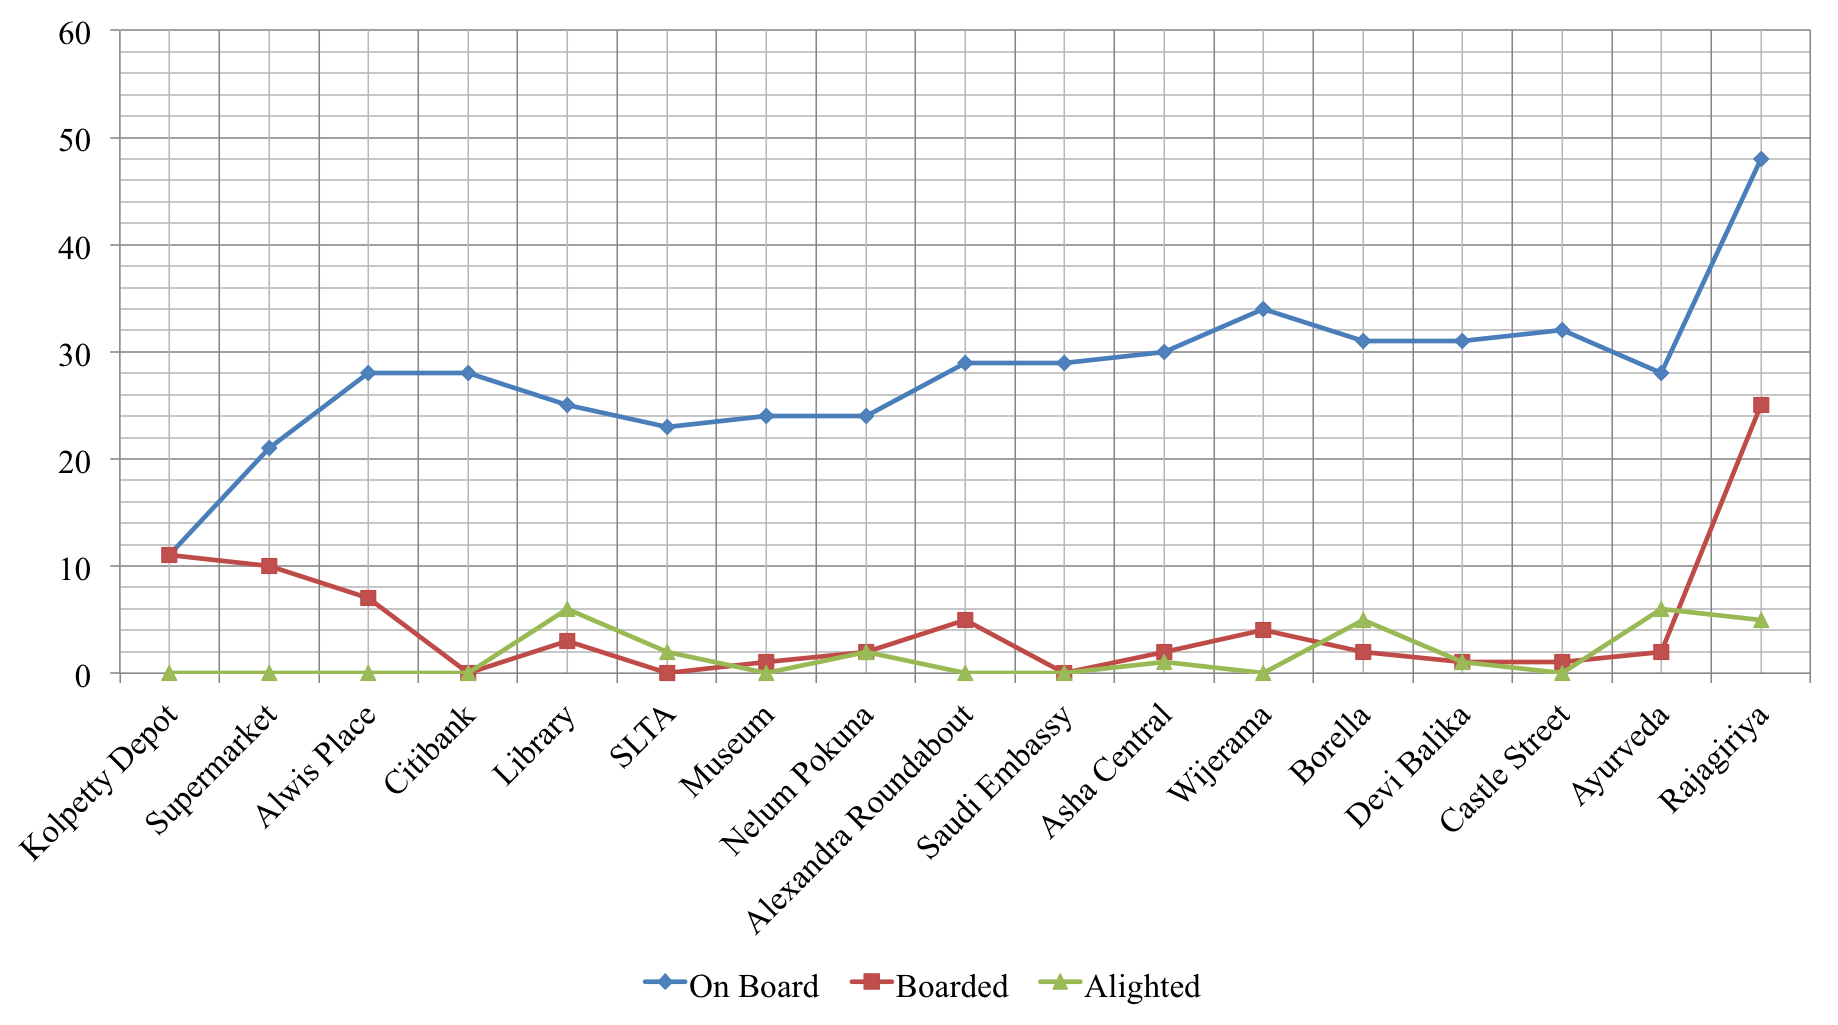
\includegraphics[scale=0.5]{passengerLoadData-Trip1}
\caption [Graph - Passenger Load Fluctuations - Trip 1] {Graph - Passenger Load Fluctuations - Trip 1}
\label {image-passengerLoadData-Trip1}
\end {figure}

\begin {figure} [h!]
\centering
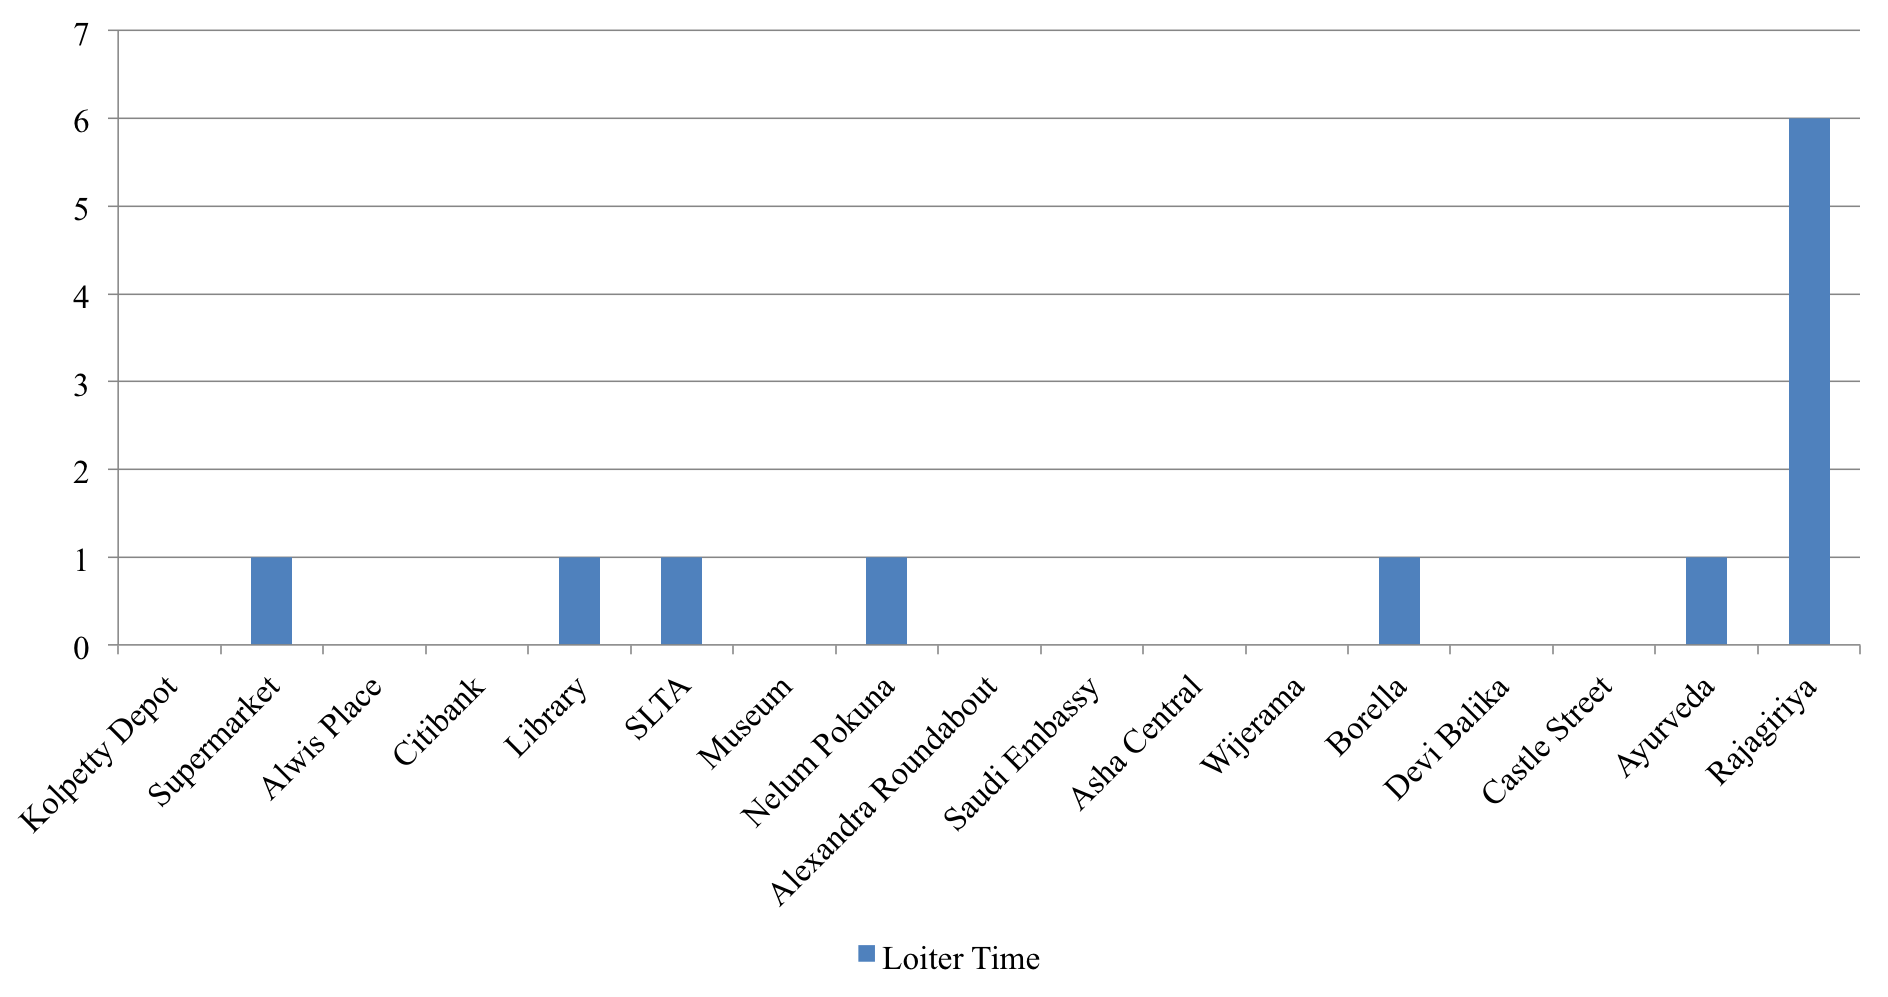
\includegraphics[scale=0.5]{loiterTimeData-Trip1}
\caption [Graph - Bus Loiter Time Data - Trip 1] {Graph - Bus Loiter Time Data - Trip 1}
\label {image-loiterTimeData-Trip1}
\end {figure}

\end{itemize}


\newpage

\section {Stakeholder Analysis}
\label {StakeholderAnalysis}

\paragraph{} The stakeholders of this Public Transport System are illustrated in Figure~\ref{image-stakeholdersDiagram}.

\begin {figure} [h!]
\centering
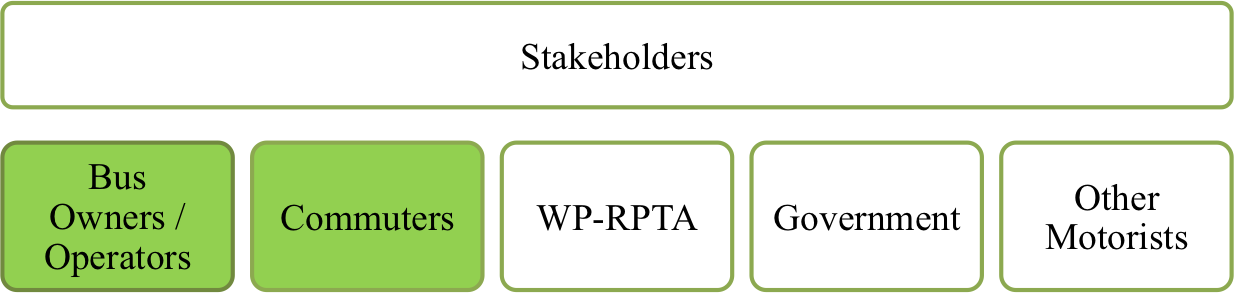
\includegraphics[scale=0.75]{stakeholdersDiagram}
\caption [Stakeholders Diagram] {Stakeholders Diagram}
\label {image-stakeholdersDiagram}
\end {figure}

\paragraph{} The most prominent stakeholders in this system are the Commuters and the Bus Owners/Operators. These 2 serve as the Demand and Supply sides of the economic equation respectively. The conflicting requirements of these two parties are illustrated in Figure~\ref{image-mainStakeholdersDiagram}.

\begin {figure} [h!]
\centering
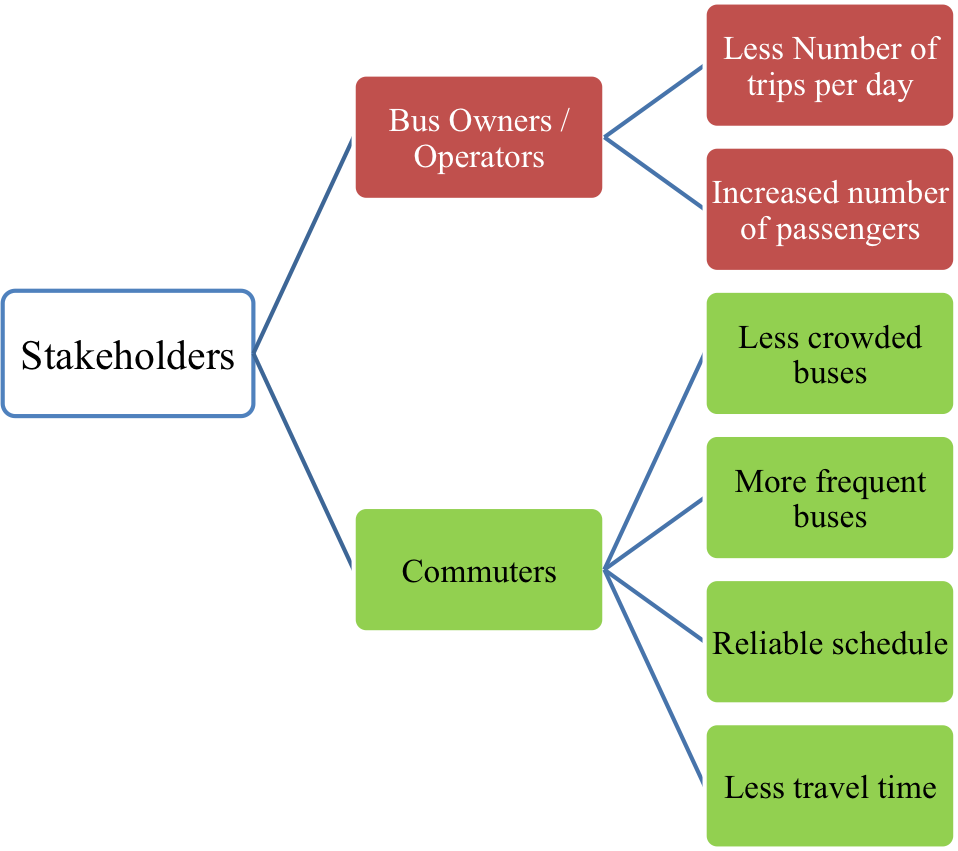
\includegraphics[scale=0.7]{mainStakeholdersDiagram}
\caption [Requirements of Main Stakeholders] {Requirements of Main Stakeholders}
\label {image-mainStakeholdersDiagram}
\end {figure}

\paragraph{} However, it is the Transport Authority that has the responsibility to keep these two parties happy. Therefore the most important stakeholder of the whole system is the Transport Authority and that is why it is important that a System is implemented that assists the Schedulers in their decision-making process. The workflow of the Scheduling Unit of the WP RPTA is comprised of 3 main stages. They are illustrated in Figure~\ref{image-timetablingProcessSteps}. The proposed Decision Support System,detailed in Chapter~\ref{chapter-ProposedSolution} will have this workflow at its core.

\begin {figure} [h!]
\centering
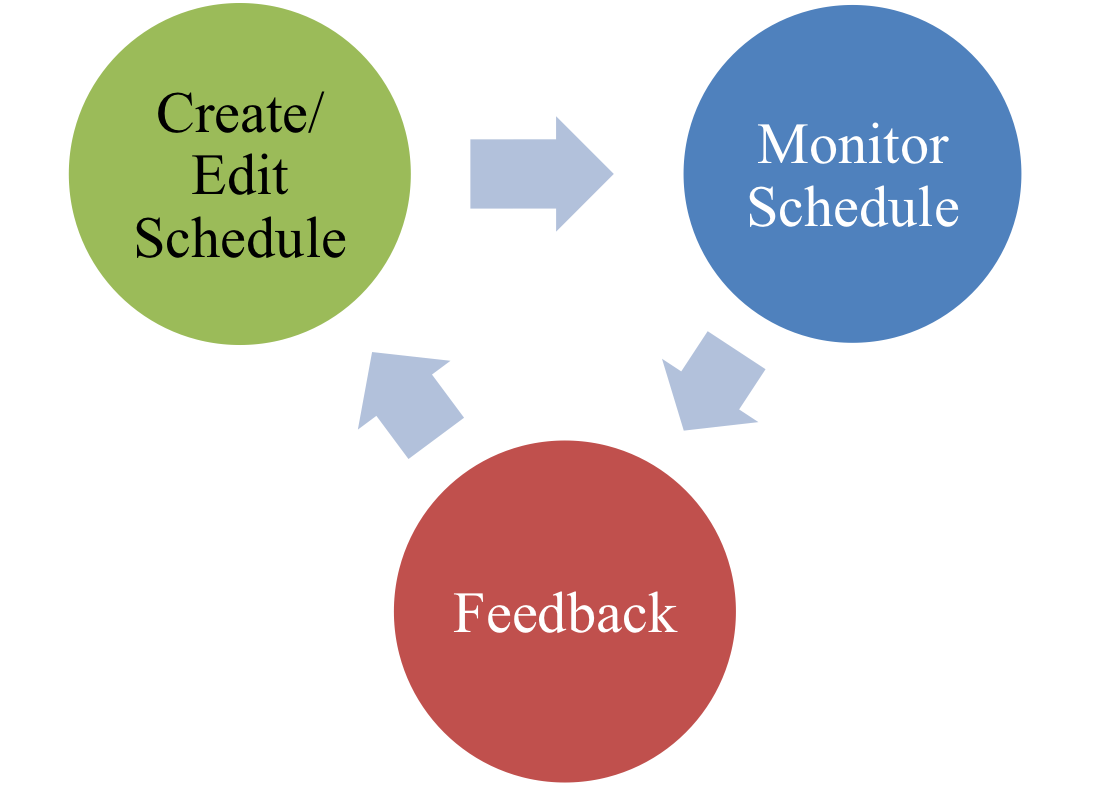
\includegraphics[scale=0.5]{timetablingProcessSteps}
\caption [Stages in the Timetabling Process Flow] {Stages in the Timetabling Process Flow}
\label {image-timetablingProcessSteps}
\end {figure}

\newpage

\section{Possible Alternative Solutions}
\label{section-Alternatives}

\paragraph{} From the contents of the current Chapter, the problems of the current system and transport service are clearly evident. From the Pilot Route Survey that was conducted, the data gathering requirements of the proposed DSS is clear.

Accordingly, possible solutions to these problems were an implementation of a Management Information System or a standalone system to create timetables for the schedulers. However neither of these really addressed all of the issues for all of the stakeholders. Management Information Systems are systems or processes that provide the information necessary to manage an organization effectively \cite{Comptroller1995, TexasAMUni2012}. Although this does accomplish the outcome of better management for the Schedulers, it does little to manage the customer-facing activities. It also focuses on management of the organization instead of aiding in the decision-making process.

Alternatively, a standalone system to merely create timetables and schedules for the bus routes does not solve all of the problems faced. Therefore, the need for a Decision Support System to aid the various stakeholders in their decision-making processes as well as enabling the proper monitoring and regulation of the service is clearly evident. The definition of a Decision Support System and how it relates to the transportation problem has already been discussed in this document. Therefore, in the next Chapter, we will see what the proposed Decision Support System is. This will include the higher-level system architecture, the system features, the main entities \& their relationships and a few screenshots of the prototype that was built for user testing.

% begin Chapter ProposedSolution

\chapter {Gaman: A solution prototype}
\label{chapter-SolutionPrototype}

\paragraph {} So far we have seen how the problem of the public transport system is structured and how it affects the stakeholders. We also saw how the nature of the problem demands a Decision Support System-like solution. This Chapter attempts to propose a DSS that deals with the public transportation problem. The architecture of the proposed system will be provided along with the proposed system features. The Chapter will end with a few UI screenshots of the prototype that was developed to test the usability and effectiveness of the functionality with the users.

\section{System Architecture}

\paragraph{ } The proposed system is designed as a web application following the client-server model. This design is the most conducive to the problem as it enables access to all stakeholders concerned in a distributed fashion. Therefore, commuters can access the system on-demand while allowing the schedulers access to the system and the data in real-time.

The prototype system used the three-tier architecture in the application. This architecture was chosen because it allowed the development of the prototype to be faster and more easily adaptable to possible requirements changes. The technologies used for the prototype are listed below,

\begin {itemize}
\item Programming Language: PHP
\item Database: MySQL
\item Versioning System: GitHub
\item UI Framework: Twitter Bootstrap
\item Theme: Flatly theme by Bootswatch (Source: http://bootswatch.com/2/flatly/)
\end {itemize}

The software architecture of the system is depicted in Figure~\ref{image-gamanSystemArchitecture}.

\begin {figure} [H]
\centering
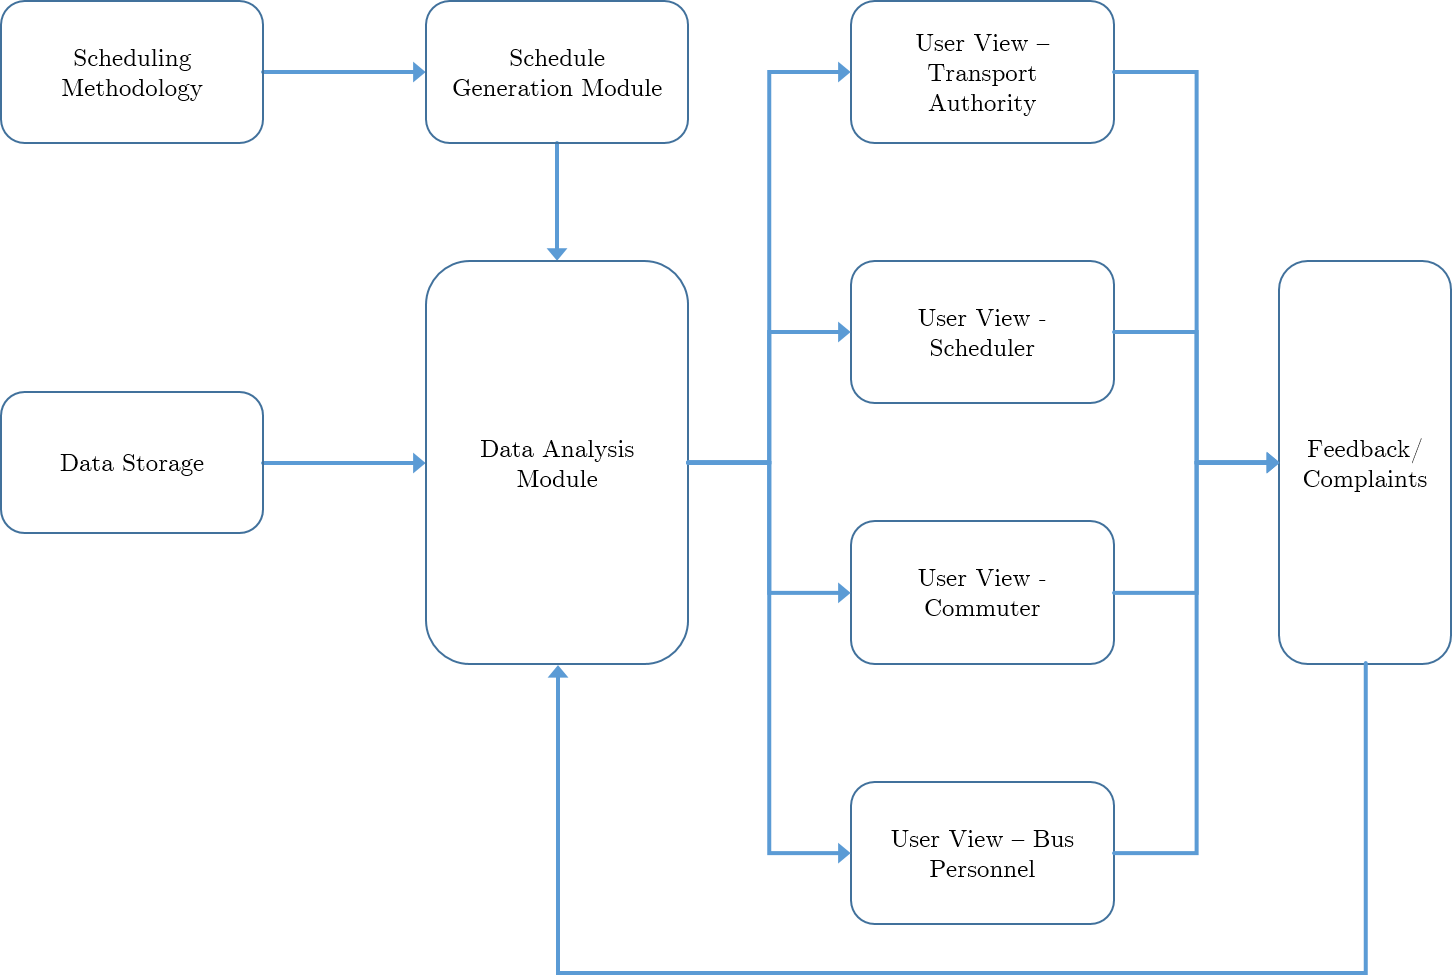
\includegraphics [scale=0.5] {gamanSystemArchitecture}
\caption [Proposed System Architecture] {Proposed System Architecture}
\label {image-gamanSystemArchitecture}
\end {figure}

The prototype that was created only included a subset of this whole architecture due to time and resource constraints. Also of note is the fact that the Data Gathering subsystem involves the data gathering infrastructure and is beyond the scope of this research project. However, it is an imperative aspect of the whole system.

\subsection{System Entities \& their Relationships}

\paragraph{} The Proposed System works with 4 main entities at it's core. They are,

\begin {itemize}
\item \textbf{Bus Routes} - Bus Routes refer to the routes that the buses provide the service on. They consist of a Beginning Bus Stop, an Ending Bus Stop and Bus Stops in between. One Bus Route may have many Stops
\item \textbf{Bus Stops} - This refers to the place allocated for a Bus to stop and drop off and/or pick up passengers. This is also known as the Bus Stand
\item \textbf{Buses} - This refers to the individual Buses that operate and provide the service to the commuters. One Bus is assigned to only one Bus Route. One Bus may have many Bus Personnel attached to it.
\item \textbf{Bus Personnel} - This refers to the people involved with the operation of the buses. This includes the Bus Driver, the Bus Conductor and the Bus Owner. In certain instances, these roles overlap. Accordingly, there may be situations where a Bus Driver is also an Owner or a Bus Conductor who is also an Owner. Each Bus Person (singular of Personnel) is assigned to only one Bus.
\end {itemize}

\paragraph{} Apart from these 4 core entities, the \textbf{Complaints} and the \textbf{General Feedback} entities are present. They exist to provide much needed feedback to the schedulers so that service quality can be maintained. These entities provide the basis for the Feedback step in the timetabling process of the schedulers (For more information regarding this process, see Figure~\ref{image-timetablingProcessSteps}).

Additionally the \textbf{Survey}, \textbf{Trip} and \textbf{Stop Activity} entities exist to aid the Survey functionality of the schedulers. A brief intro into what these entities are is listed below,

\begin {itemize}
\item \textbf{Survey} - An investigation of the buses in a route in terms of the passenger loads on the buses plying on that route. These are called route surveys and the Schedulers say ascertain the passenger loads as input for the timetabling through this process. One Survey is conducted on only one route at a time.
\item \textbf{Trip} - A trip is one-way journey between the Beginning Stop and the Ending Stop of a Bus Route. A Survey has many Trips included. Within the Trip, there are many Stops, and consequently many Stop Activities.
\item \textbf{Stop Activity} - A Stop Activity is the record of the exchanges of passengers that occurs at a Bus Stop during a Trip. 4 main facts are recorded for a Stop Activity when the bus stops at a Bus Stop. The number of passengers who get off the bus, number of people that get on the bus, the time (timestamp) the bus came to a stop and the passengers started to get off the bus at the Bus Stop and finally the time (timestamp) the bus departed the Bus Stop.
\end {itemize}

The above mentioned entities allow the Schedulers to carry out a route survey and gather the necessary data for the timetabling process. The Route Surveys that the Schedulers perform are imperative in their timetable formulation as it acts as the data input for the process. The Schedulers mainly obtain the Passenger Load information which is directly related to the dispatching of buses on a route. Loiter time data is also used to identify errant bus operators as well as to continuously monitor the total travel time on a route.



\section{System Features}
\label{systemFeatures}

\paragraph{ } The list of system features and functionality is noted below. Please note, the features marked under \textit{Public} is available for the regular commuters to access while the functionality marked under \textit{Admin} is only available for the Schedulers and other administrative staff at the Transport Authority.

\begin{itemize}

\item Public Functions
\begin{itemize}
\item \textbf{Information Portal for Bus Routes, Stops, Buses and Bus Personnel} - This is, as its name suggests, the functionality of providing the data about the 4 main entities related to the transportation service in a smile easy-to-use, easy-to-read-and-understand interface. The information includes the basics from name of stop (for Bus Stops) and the Stops along a particular route (for Bus Routes) to more advanced things like the Personnel assigned to a particular Bus and the number of complaints received on a particular Bus.
\item \textbf{Information Portal for Bus Fares} - This would basically provide the details of the Bus fares in a given route.
\item \textbf{Bus Route Finder functionality} - When an origin and destination stop are given, the user is presented with a list of bus routes to take
\item \textbf{Submitting and reviewing submitted General Feedback} - Using this functionality, users can provide comments (good or bad) regarding the 4 main entities. This goes hand in hand with the Complaints and acts as a complimenting function to the Complaints.
\item \textbf{Submitting and reviewing submitted Complaints} - Users can submit their complaints to the authority and these will be investigated and action taken. The Complaints also acts as a notification for the Schedulers in their timetabling process. For instance when there are a lot of complaints on a particular route regarding overcrowded buses or consistently delayed buses, the Schedulers can reconsider the timetable for that route and improve it. Currently this connection between the Complaints and the Schedulers is not available and therefore the Schedulers have no idea which areas need improvement.
\end{itemize}

\item Admin Functions
\begin{itemize}
\item \textbf{Survey data storage, retrieval and visualization} - this is one of the main functionalities of the proposed system. it provides the knowledge base as well as the main input to the timetabling process of the Schedulers.
\item \textbf{Timetable Storage, Retrieval and Visualization} - Timetables are documents that the buses are dispatched according to. The tracking of buses according to their dispatch times is currently done manually. The times that the buses are dispatched are recorded on timetable and sent in to the regional offices. This functionality of the system attempts to digitize that by having a digital representation of the data so that it can be stored and retrieved later.
\item \textbf{Timetable Generation} - This functionality enables the schedulers to automatically generate timetables for a given route. As mentioned previously, this is currently done manually and the proposed system would incorporate a the feature of generating the timetable by calculating the average headways.
\item \textbf{Vehicle and Crew Scheduling} - This is the next step in the planning process. The Vehicle and Crew Scheduling functions are the rosters that the bus operators follow. This function enables the Schedulers to automatically generate these without having to do this step of the process manually.
\item \textbf{Complaint and General Feedback tracking Dashboard} - The Complaint and General Feedback functions serve as the indicator in this system. It tells the Schedulers which routes are doing well and which ones aren't, which buses are breaking the law and which bus personnel has a good record. It allows the authority to analyze the quality of the service and includes the commuters in the process of measuring service quality.
\end{itemize}

\end{itemize}



\section{URL of prototype system}

\paragraph{} The prototype system can be found at the following URL: \url{http://gaman.byethost4.com/}. The system's Admin Interface can be found at \url{http://gaman.byethost4.com/admin/}. The login credentials for both these interfaces are listed below.

\begin {itemize}

\item Public Area
\begin {itemize}
\item Username: \textbf{heisenberg}
\item Password: \textbf{123}
\end {itemize}

\item Admin area
\begin {itemize}
\item Username: \textbf{admin}
\item Password: \textbf{123}
\end {itemize}

\end {itemize}

The system is an active project on GitHub. The code repository can be found at, \url{https://github.com/afthaj/Gaman/}



\section{UI Screenshots}

\paragraph{} UI Screenshots of the prototype system are displayed below.

\begin {figure} [H]
\centering
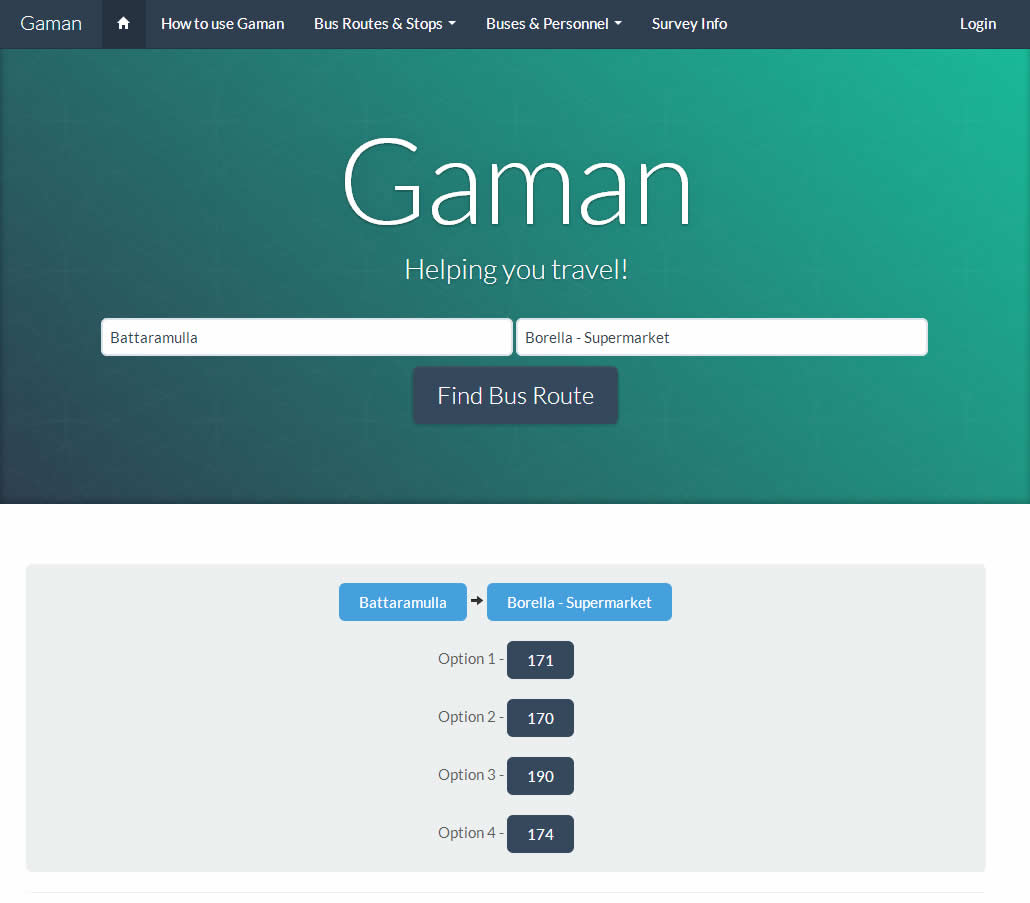
\includegraphics[scale=0.4]{public-home}
\caption [Screenshot - Public Home Page] {Screenshot - Public Home Page}
\label {image-public-home}
\end {figure}

\begin {figure} [H]
\centering
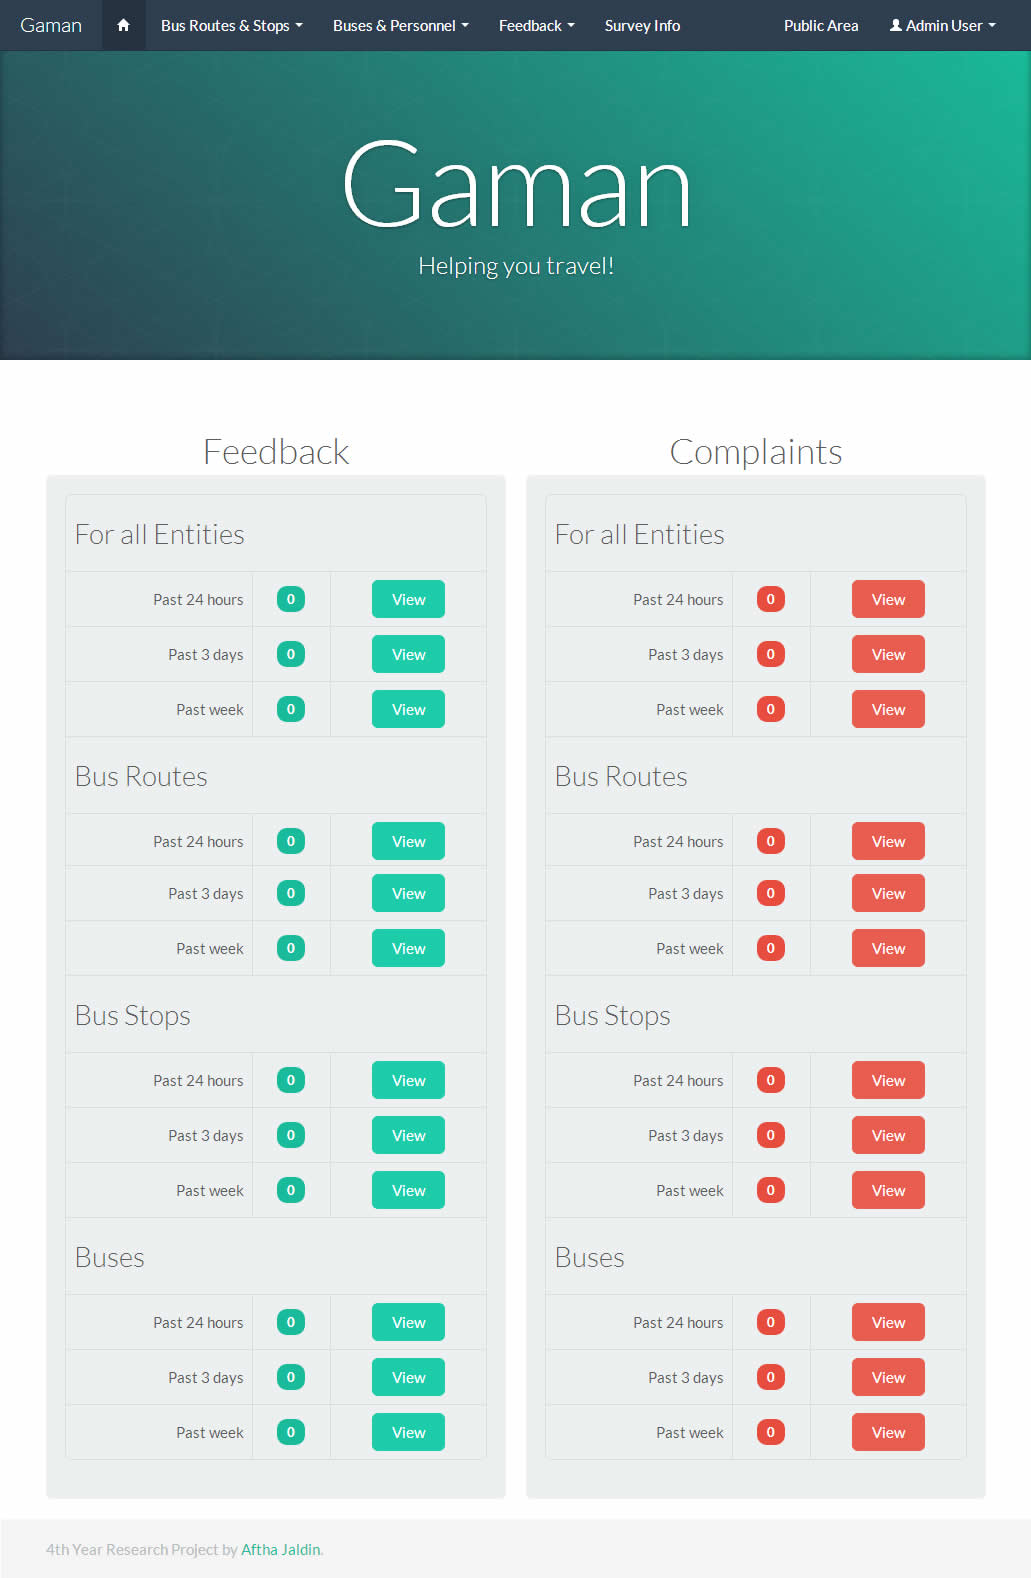
\includegraphics[scale=0.4]{admin-home}
\caption [Screenshot - Admin Home Page] {Screenshot - Admin Home Page}
\label {image-admin-home}
\end {figure}

\begin {figure} [H]
\centering
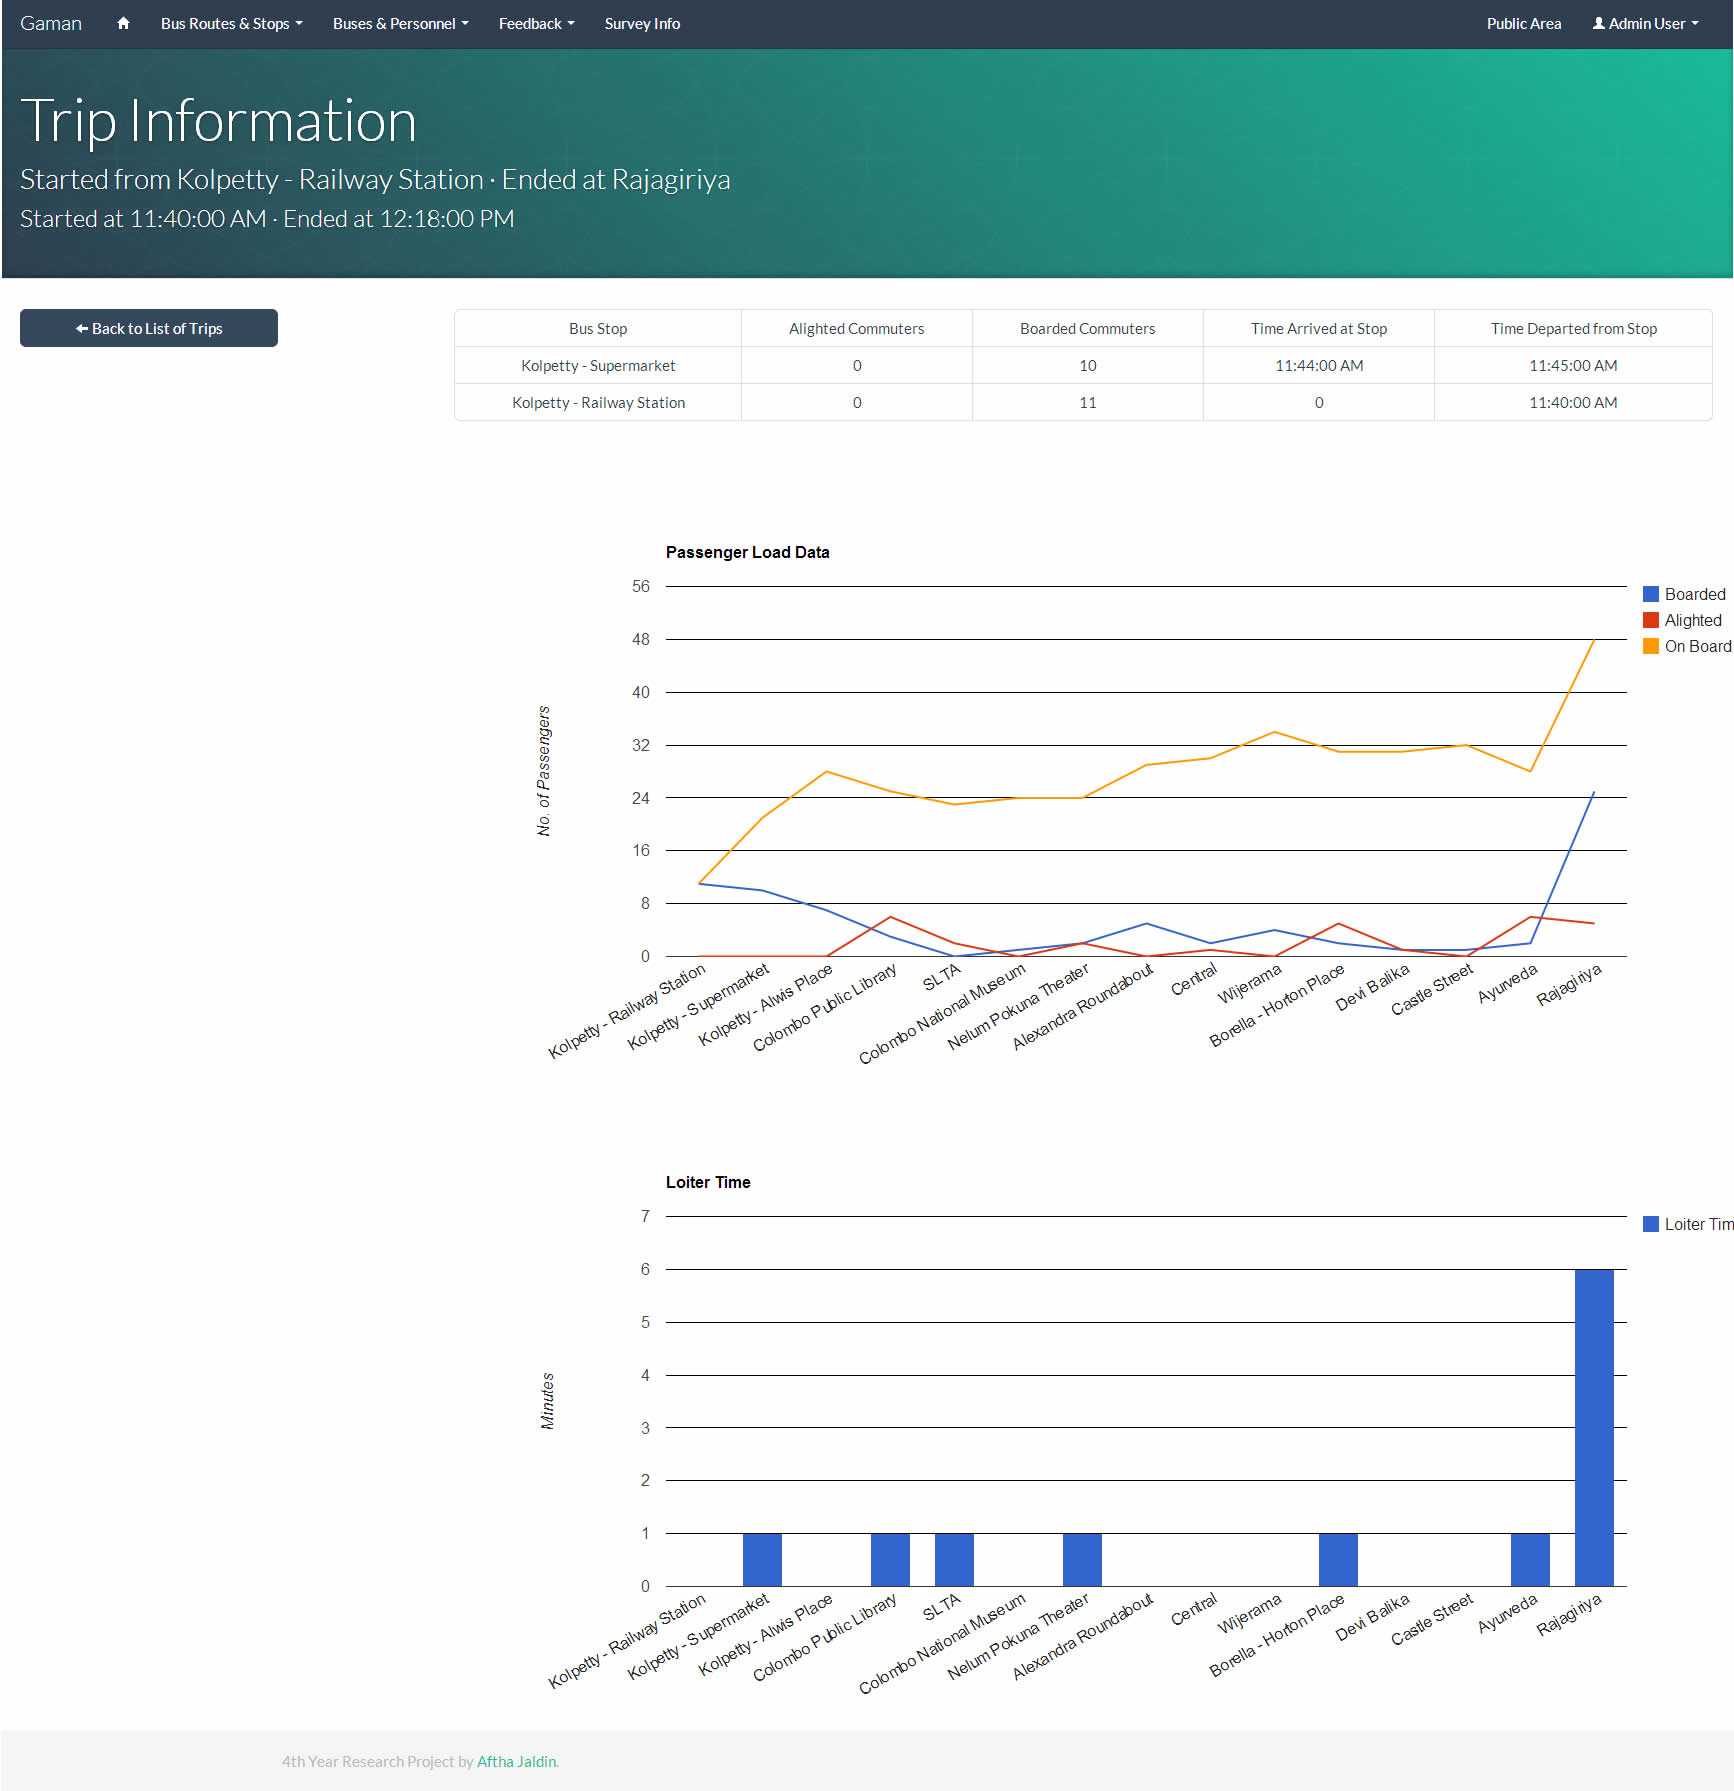
\includegraphics[scale=0.25]{admin-trip-information}
\caption [Screenshot - ] {Screenshot - }
\label {image-admin-trip-information}
\end {figure}

\begin {figure} [H]
\centering
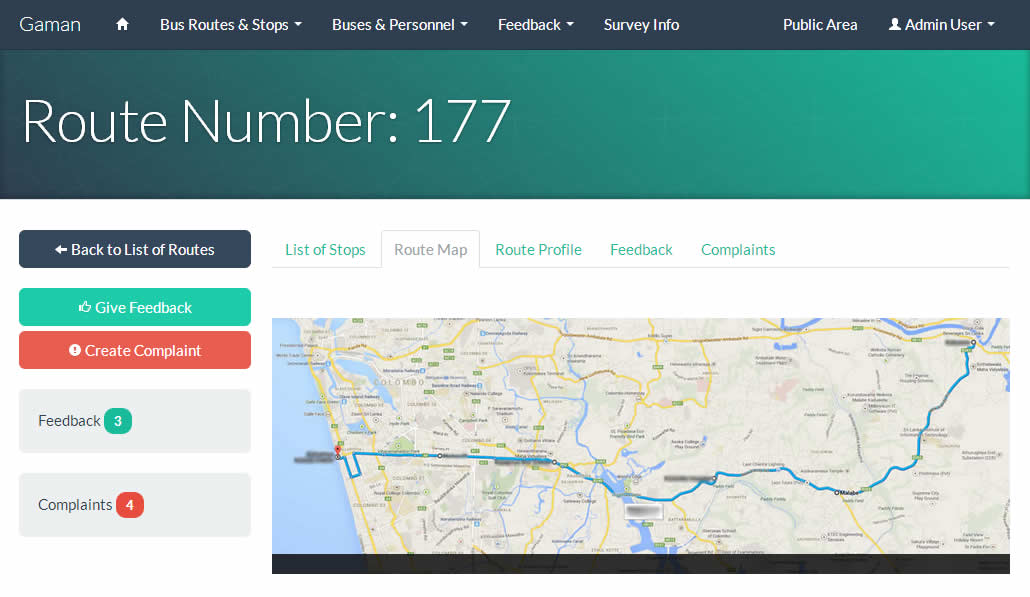
\includegraphics[scale=0.4]{admin-view-route}
\caption [Screenshot - ] {Screenshot - }
\label {image-admin-view-route}
\end {figure}

\begin {figure} [H]
\centering
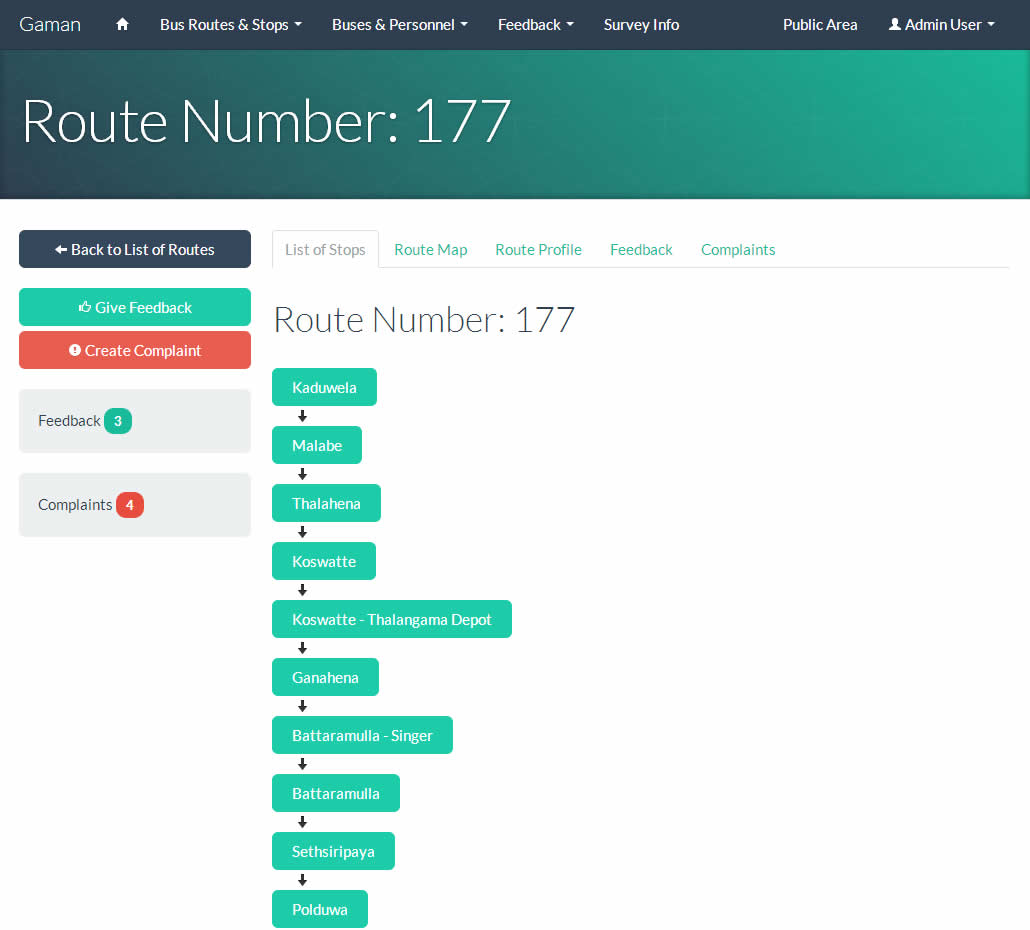
\includegraphics[scale=0.4]{admin-view-route-2}
\caption [Screenshot - ] {Screenshot - }
\label {image-admin-view-route-2}
\end {figure}

\begin {figure} [H]
\centering
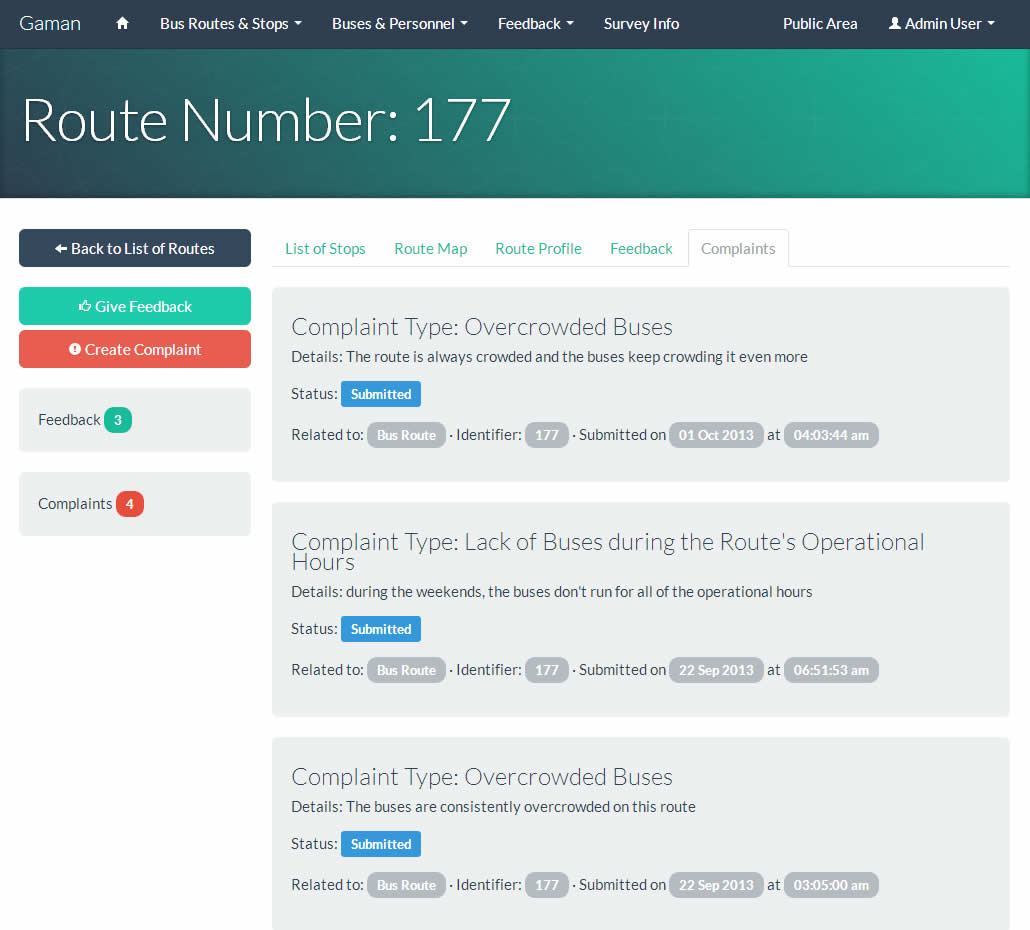
\includegraphics[scale=0.4]{admin-view-route-3}
\caption [Screenshot - ] {Screenshot - }
\label {image-admin-view-route-3}
\end {figure}

\begin {figure} [H]
\centering
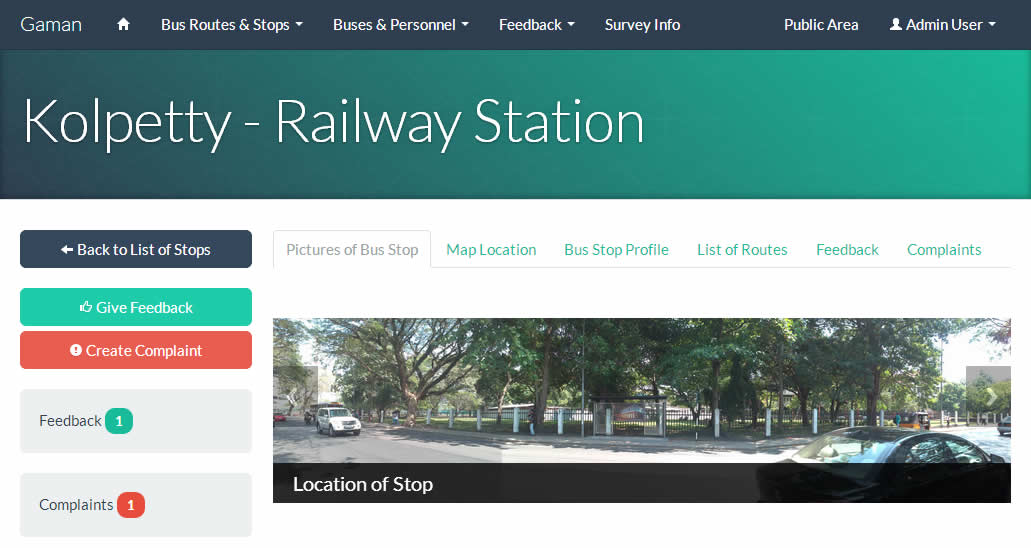
\includegraphics[scale=0.4]{admin-view-stop}
\caption [Screenshot - ] {Screenshot - }
\label {image-admin-view-stop}
\end {figure}

\begin {figure} [H]
\centering
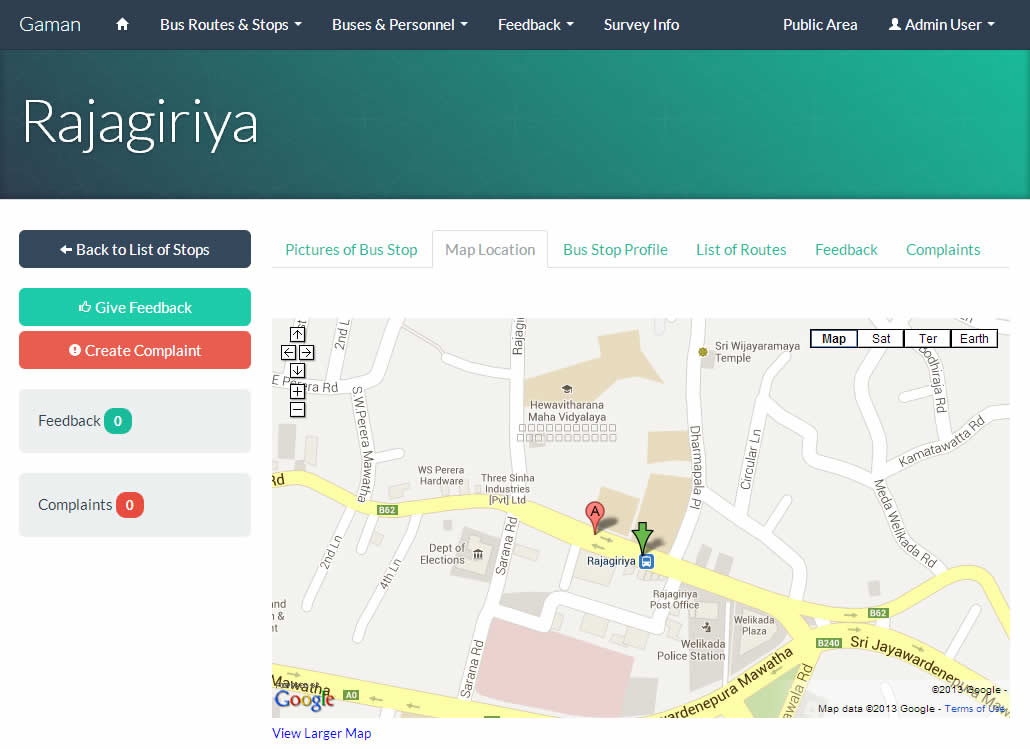
\includegraphics[scale=0.4]{admin-view-stop-2}
\caption [Screenshot - ] {Screenshot - }
\label {image-admin-view-stop-2}
\end {figure}

\begin {figure} [H]
\centering
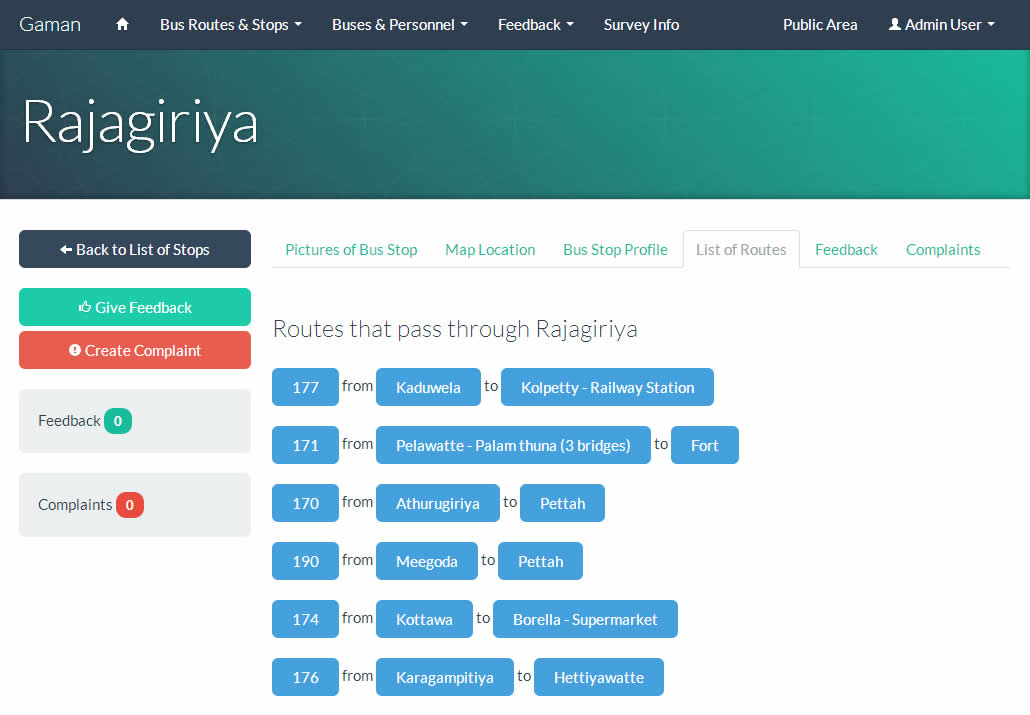
\includegraphics[scale=0.4]{admin-view-stop-3}
\caption [Screenshot - ] {Screenshot - }
\label {image-admin-view-stop-3}
\end {figure}

\begin {figure} [H]
\centering
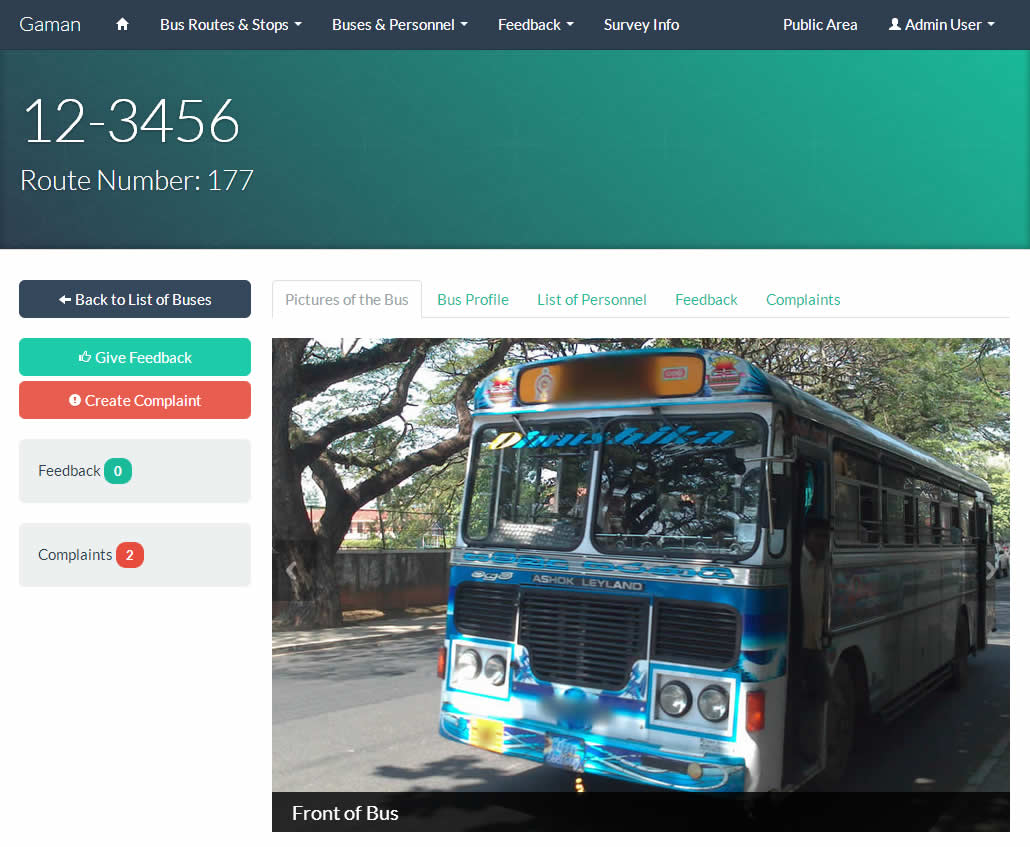
\includegraphics[scale=0.4]{admin-view-bus}
\caption [Screenshot - ] {Screenshot - }
\label {image-admin-view-bus}
\end {figure}

\begin {figure} [H]
\centering
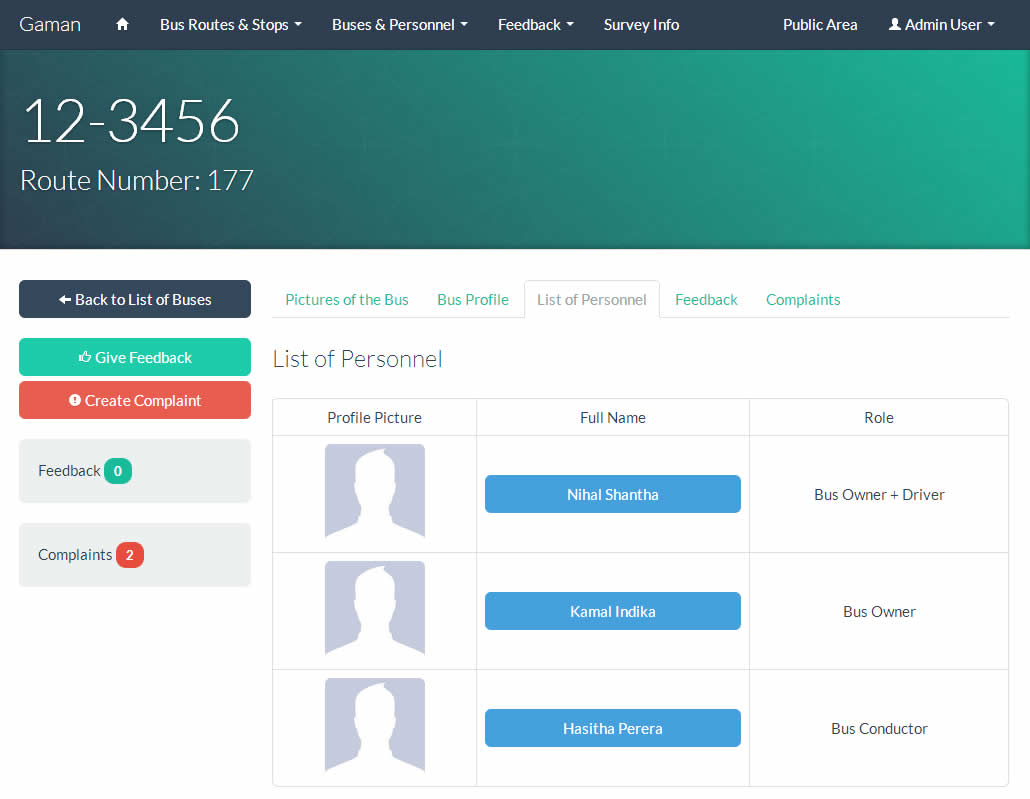
\includegraphics[scale=0.4]{admin-view-bus-2}
\caption [Screenshot - ] {Screenshot - }
\label {image-admin-view-bus-2}
\end {figure}

\begin {figure} [H]
\centering
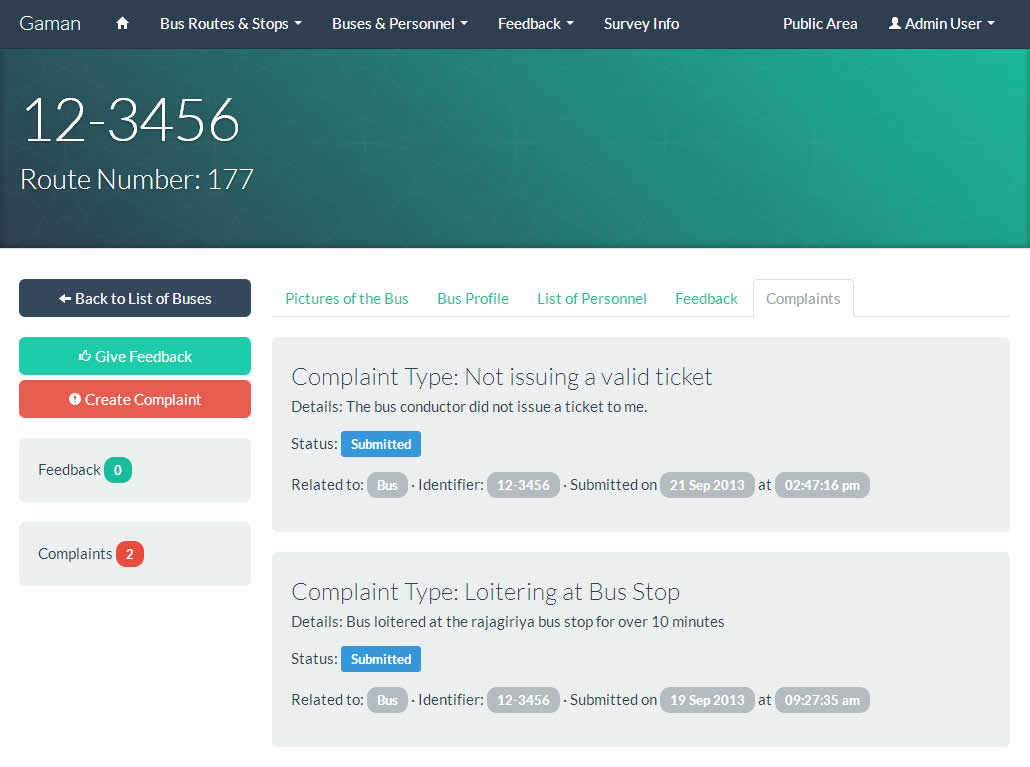
\includegraphics[scale=0.4]{admin-view-bus-3}
\caption [Screenshot - ] {Screenshot - }
\label {image-admin-view-bus-3}
\end {figure}

\begin {figure} [H]
\centering
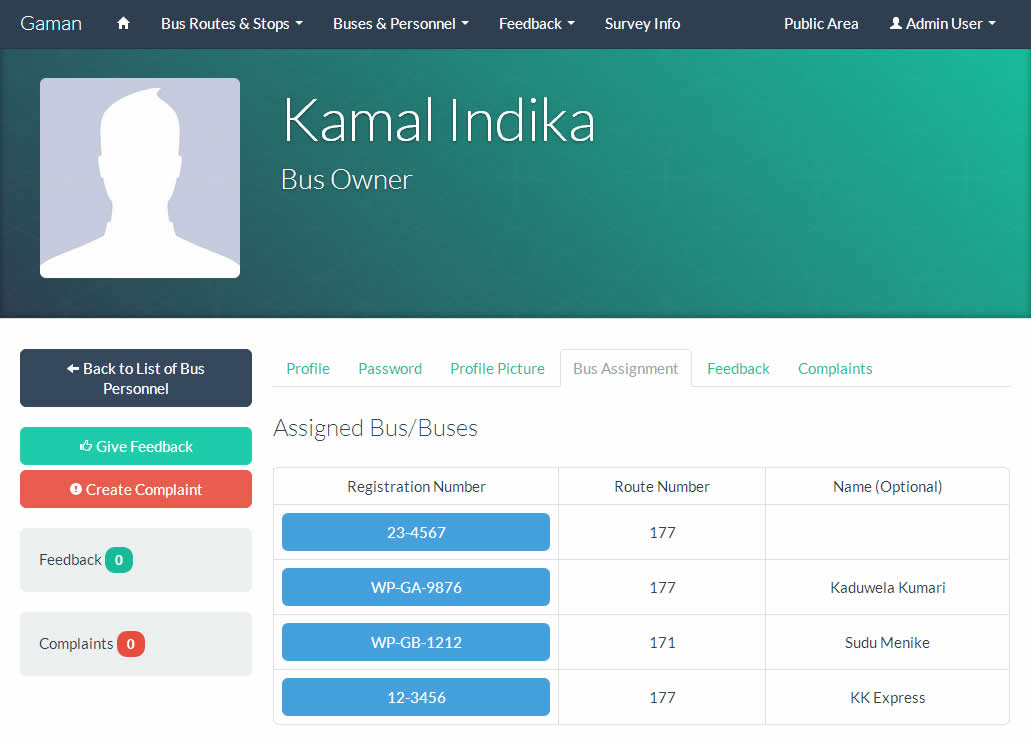
\includegraphics[scale=0.4]{admin-view-bus-personnel}
\caption [Screenshot - ] {Screenshot - }
\label {image-admin-view-bus-personnel}
\end {figure}

\begin {figure} [H]
\centering
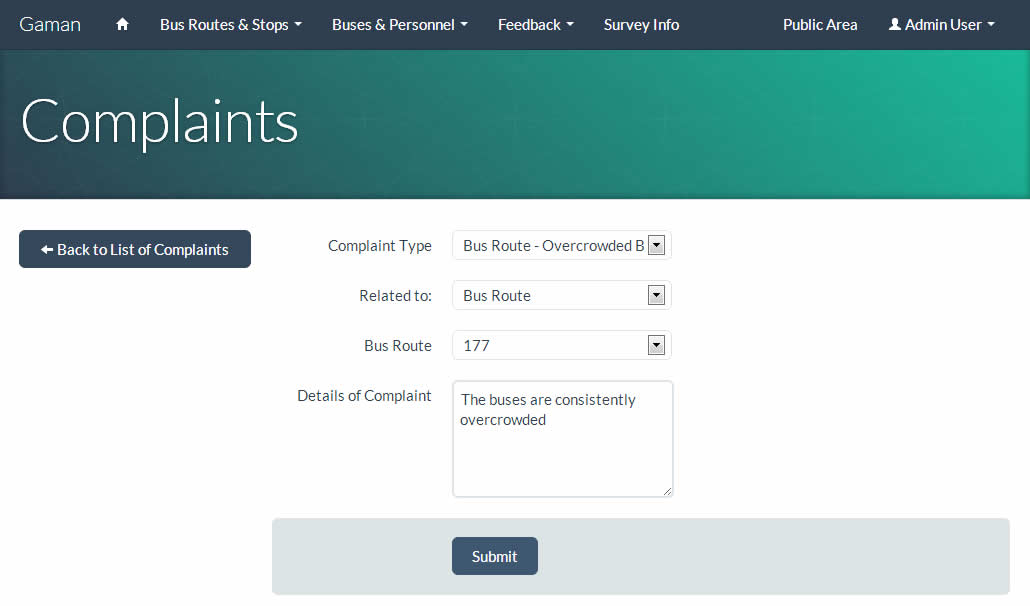
\includegraphics[scale=0.4]{admin-add-complaint}
\caption [Screenshot - ] {Screenshot - }
\label {image-admin-add-complaint}
\end {figure}

\begin {figure} [H]
\centering
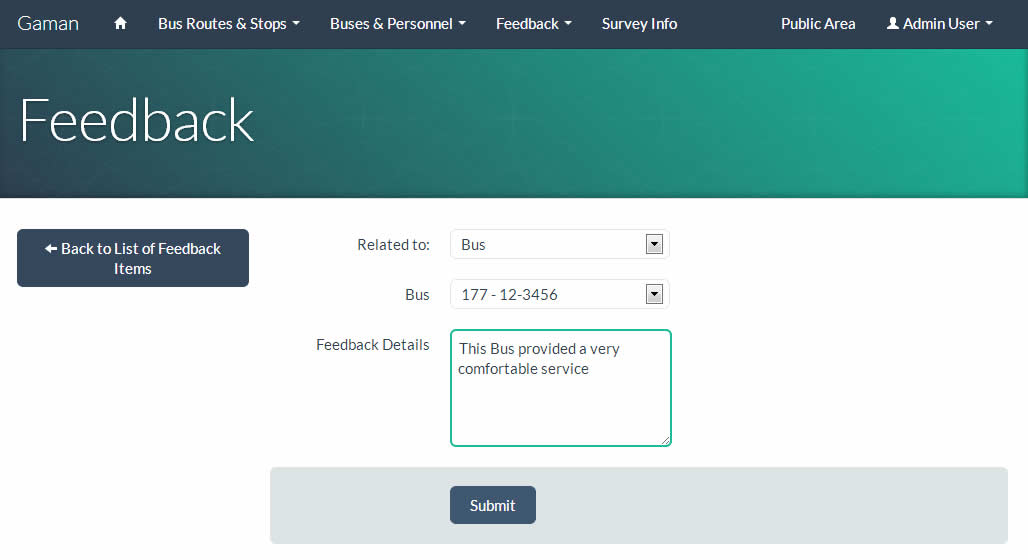
\includegraphics[scale=0.4]{admin-add-feedback}
\caption [Screenshot - ] {Screenshot - }
\label {image-admin-add-feedback}
\end {figure}



\section{Testing the prototype}

\paragraph{} 






% begin Chapter ResearchEvaluation

\chapter {Research Evaluation}
\label{chapter-ResearchEvaluation}

\paragraph {} In the previous chapter, we took a look at the proposed system architecture and it's features. We also understood what the entities in the system were and how they relate to each other. In any research, the evaluation of the concept is as, if not more, important to the justifying the end result. Accordingly an evaluation of the prototype was carried out with the schedulers and the commuters.

\section{User Evaluation of Prototype}

\paragraph{} There are 3 main types of users that used this research prototype. They are,

\begin{itemize}
\item Schedulers of the Transport Authority
\item Commuters
\item Bus Owners and Operators
\end{itemize}

\paragraph{} Of these 3 main types of users, the Schedulers act as the Admins and they can carry out the Admin functionalities listed under Section~\ref{systemFeatures}. Each of these users will have different views and functionalities associated with them. The User evaluation was carried out only with the Schedulers and the Commuters as I was unable to find any Bus Owners / Operators willing to participate in this study.

The prototype was hosted on a free hosting service and the Schedulers were interviewed while they were using the system to obtain a qualitative feedback on the prototype and its functionality. The URL of the public interface was sent to regular commuters to ascertain their feedback on the system. The prototype system can be accessed at \url{http://gaman.byethost4.com/}.

\subsection{Feedback of the Schedulers}

\paragraph{} The feedback from the schedulers was overwhelmingly positive towards the system. They said they welcome a system like this and would gladly use it if it does eventually become a system ready for implementation. Furthermore, they mentioned that the User Interface was very simple, easy-to-use and intuitive.

The Schedulers also pointed out that an implementable system would need some added functionality such as the ability to store timetables, generate timetables automatically when given the data and the vehicle and crew scheduling functionalities. However, they said as this is a prototype system, the concept is correct, sound and suitable for further development. (Source: Interviews with the Scheduling Officers of the WP RPTA)

\subsection{Feedback of the Commuters}

\paragraph{} After hosting the prototype online, a group of commuters were provided the link and given an explanation on how to use the system. Then they were asked to fill out a survey on their experience using the Gaman prototype system. The key points have been summarized and the results have been tabulated below. The Survey can be accessed at the following URL: \url{https://docs.google.com/forms/d/100pWQ4476Mo4tqn3SHLmVO1r8cB-ayuQEdai8xWyjCI/viewform/}

\begin {itemize}

\item Number of Participants: 39

\item Age group - Table~\ref{table-survey-ageGroupOfSurveyParticipants}

\begin{table} [h]
\centering
\begin{tabular}{|l|c|}
\hline
Age Group & Number of participants \\
\hline
20-35	&38 \\
10-19	&01 \\
\hline
\end{tabular}
\caption{Age Groups of Participants}
\label{table-survey-ageGroupOfSurveyParticipants}
\end{table}

\item Frequency of travel in the bus - Table~\ref{table-survey-frequencyOfTravelInTheBus}

\begin{table} [h]
\centering
\begin{tabular}{|l|c|}
\hline
Frequency of travel & Number of participants \\
\hline
Daily, one or two times a day	&20 \\
Daily, several times a day	&15 \\
A few times a week	&03 \\
A few times a month	&01 \\
\hline
\end{tabular}
\caption{Frequency of travel in the bus}
\label{table-survey-frequencyOfTravelInTheBus}
\end{table}

\item Rating - Information Portal (Scale of 1 to 5 with 5 being "Very Useful" and 1 being "Not useful at all") - Table~\ref{table-survey-rating-InformationPortal} - Figure~\ref{image-ratingInformationPortal}

\item Qualitative comments received
\begin {itemize}
\item "well i think infomation about bus routes is useful if we want to travel to a place that we dnt know using bus routes. most of the time i use google maps to navigate but it doesnt provide me the functionality of which bus route should i take. so i think this is a good effort"
\item "useful."
\item "It is a superb move. Very informative and useful. Hope this is mobile friendly as well."
\item "Very helpful. There are sufficient information regarding buses and bus routes and personals."
\item "It is great that we can use this system to get information about the buses and owners."
\item "Really good one"
\end {itemize}

\item Rating - Bus Route Finder (Scale of 1 to 5 with 5 being "Very Useful" and 1 being "Not useful at all") - Table~\ref{table-survey-rating-BusRouteFinder} - Figure~\ref{image-ratingBusRouteFinder}

\item Qualitative comments received
\begin {itemize}
\item "simple but effective solution to easily find the routes."
\item "It's better if the information were presented in a better way, so that those can be found easily (E.g. provide searching facilities etc.)"
\item "More places need to be added to the system. It's better to give the bus route with the start and end destination as the first details. for some users sometimes giving only route number will not make sense very much."
\end {itemize}

\item Rating - Feedback Functionality (Scale of 1 to 5 with 5 being "Very Useful" and 1 being "Not useful at all") - Table~\ref{table-survey-rating-FeedbackFunctionality} - Figure~\ref{image-ratingFeedbackFunctionality}

\item Qualitative comments received
\begin {itemize}
\item "Needs the ability to connect drivers and conductors to buses,feedbacks and complaints. drivers and conducters may get assigned to the buses by a time table component. ( couldn't test this since i couldn't see the needed form elements for filling those info while giving feedback )"
\item "Feedback to drivers and conductors may not reach them because of the low computer literacy. However, if there is any responsible person to handle or communicate with them then it is really useful function"
\end {itemize}

\item Rating - Comlaints Functionality (Scale of 1 to 5 with 5 being "Very Useful" and 1 being "Not useful at all") - Table~\ref{table-survey-rating-ComplaintsFunctionality} - Figure~\ref{image-ratingComplaintsFunctionality}

\item Qualitative comments received
\begin {itemize}
\item "This is a very useful functionality that would help in increasing and maintaining the quality of the bus services."
\item "This is really good because sometimes we have to bare all the sh***y experiences or will be able to share it with few friends and forget about those. But this functionality facilitates us to share our good/bad experiences with others and even will be able to do something."
\item "It's very useful to have such functionality, because that is one of  the main problem we can see in the public transport system in Sri Lanka."
\item "I wish the complain data were more specific. For example, user might be interested in knowing the bus-route associated with a certain complain or he might be interested viewing all the complains related to a certain but-route."
\item "If it functioned properly this will have a big impact. Simply a user can share their own experience. But there are possibilities of fake complaints."
\end {itemize}

\item Rating - User Interface (Scale of 1 to 5 with 5 being "Very easy to use" and 1 being "Very difficult to use") - Table~\ref{table-survey-rating-UserInterface} - Figure~\ref{image-ratingUserInterface}

\item Qualitative comments received
\begin {itemize}
\item "good. but can improve. trade off between simplicity and ease of use."
\item "Simple and nice! good work!"
\item "Simple, but effective and attractful. Nicely developed."
\item "Looks a bit too linear in my opinion... more vibrant colours should be used to highlight the important and most frequently used features.."
\item "I like the simplest interface and colors. Some pages have textboxes whichs seems very small comparing to the screen size. Better if you add some autoresize them"
\end {itemize}

\item Survey Question - Would you use a system like this if it was implemented? - Table~\ref{table-survey-question-WouldYouUseASystemLikeThis} - Figure~\ref{image-questionWouldYouUse}

\begin{table} [h]
\centering
\begin{tabular}{|l|c|}
\hline
Rating & Number of participants \\
\hline
5	&09 \\
4	&20 \\
3	&07 \\
2	&03 \\
1	&00 \\
\hline
\end{tabular}
\caption{Rating - Information Portal}
\label{table-survey-rating-InformationPortal}
\end{table}

\begin {figure} [h]
\centering
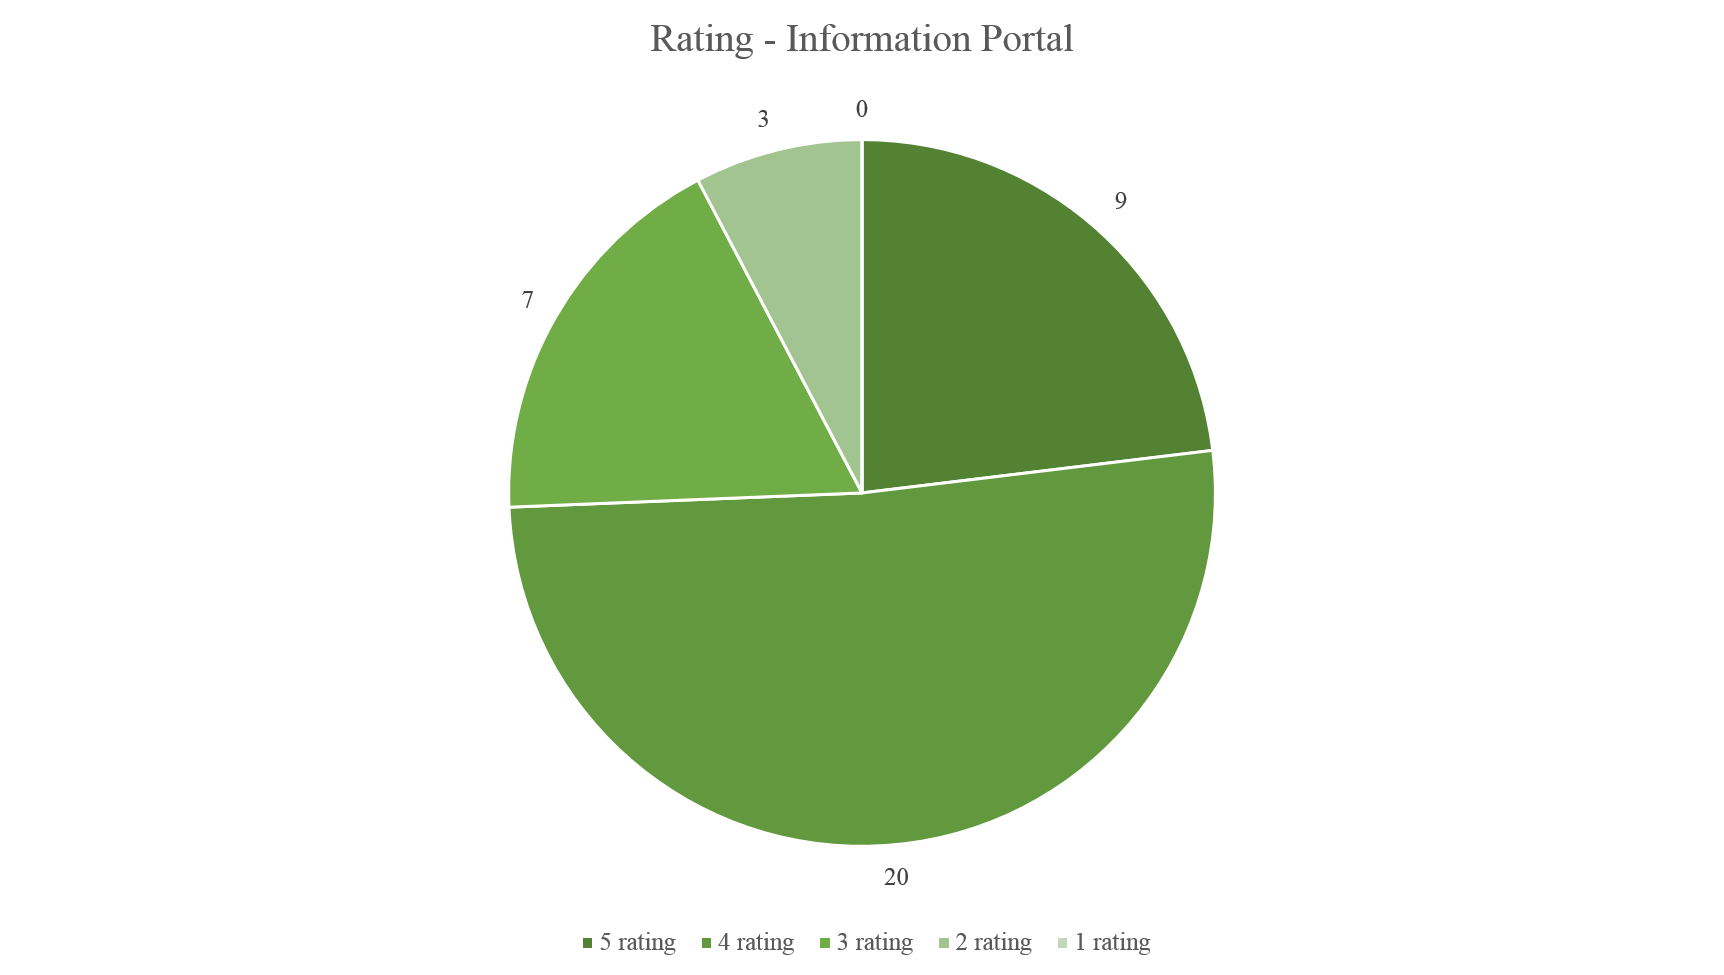
\includegraphics [scale=0.5] {ratingInformationPortal}
\caption [Chart - Rating - Information Portal] {Chart - Rating - Information Portal}
\label {image-ratingInformationPortal}
\end {figure}

\begin{table} [h]
\centering
\begin{tabular}{|l|c|}
\hline
Rating & Number of participants \\
\hline
5	&12 \\
4	&16 \\
3	&09 \\
2	&02 \\
1	&01 \\
\hline
\end{tabular}
\caption{Rating - Bus Route Finder}
\label{table-survey-rating-BusRouteFinder}
\end{table}

\begin {figure} [h]
\centering
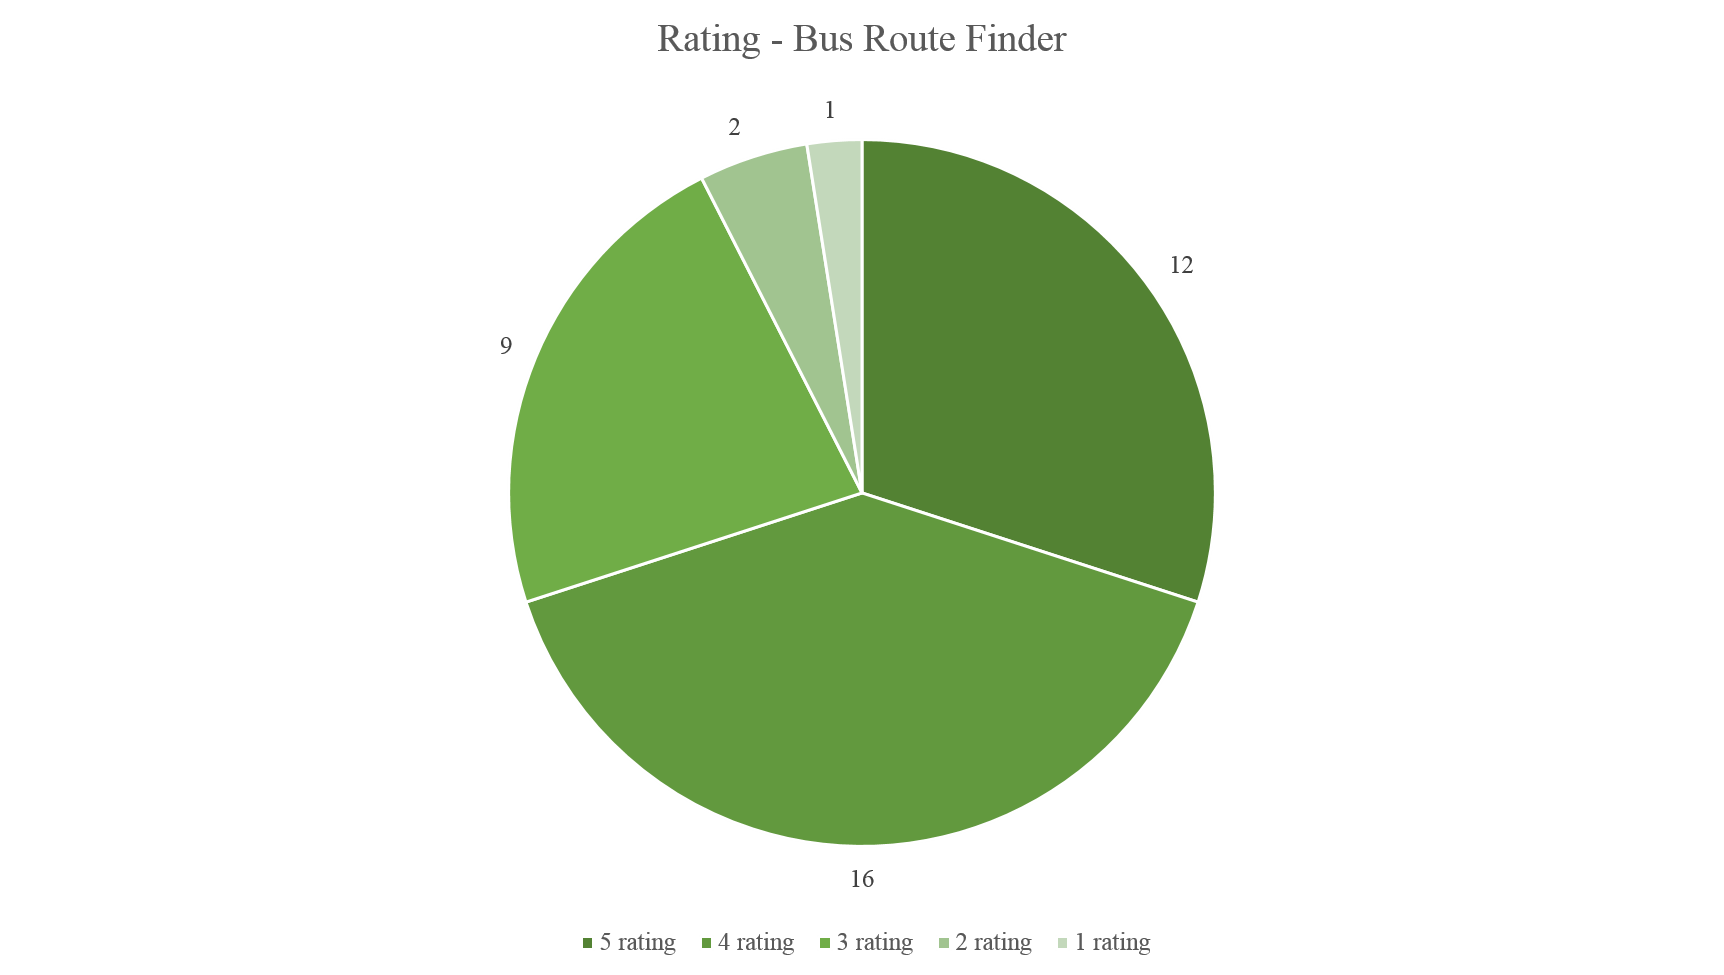
\includegraphics [scale=0.5] {ratingBusRouteFinder}
\caption [Chart - Rating - Bus Route Finder] {Chart - Rating - Bus Route Finder}
\label {image-ratingBusRouteFinder}
\end {figure}

\begin{table} [h]
\centering
\begin{tabular}{|l|c|}
\hline
Rating & Number of participants \\
\hline
5	&09 \\
4	&14 \\
3	&13 \\
2	&03 \\
1	&00 \\
\hline
\end{tabular}
\caption{Rating - Feedback Functionality}
\label{table-survey-rating-FeedbackFunctionality}
\end{table}

\begin {figure} [h]
\centering
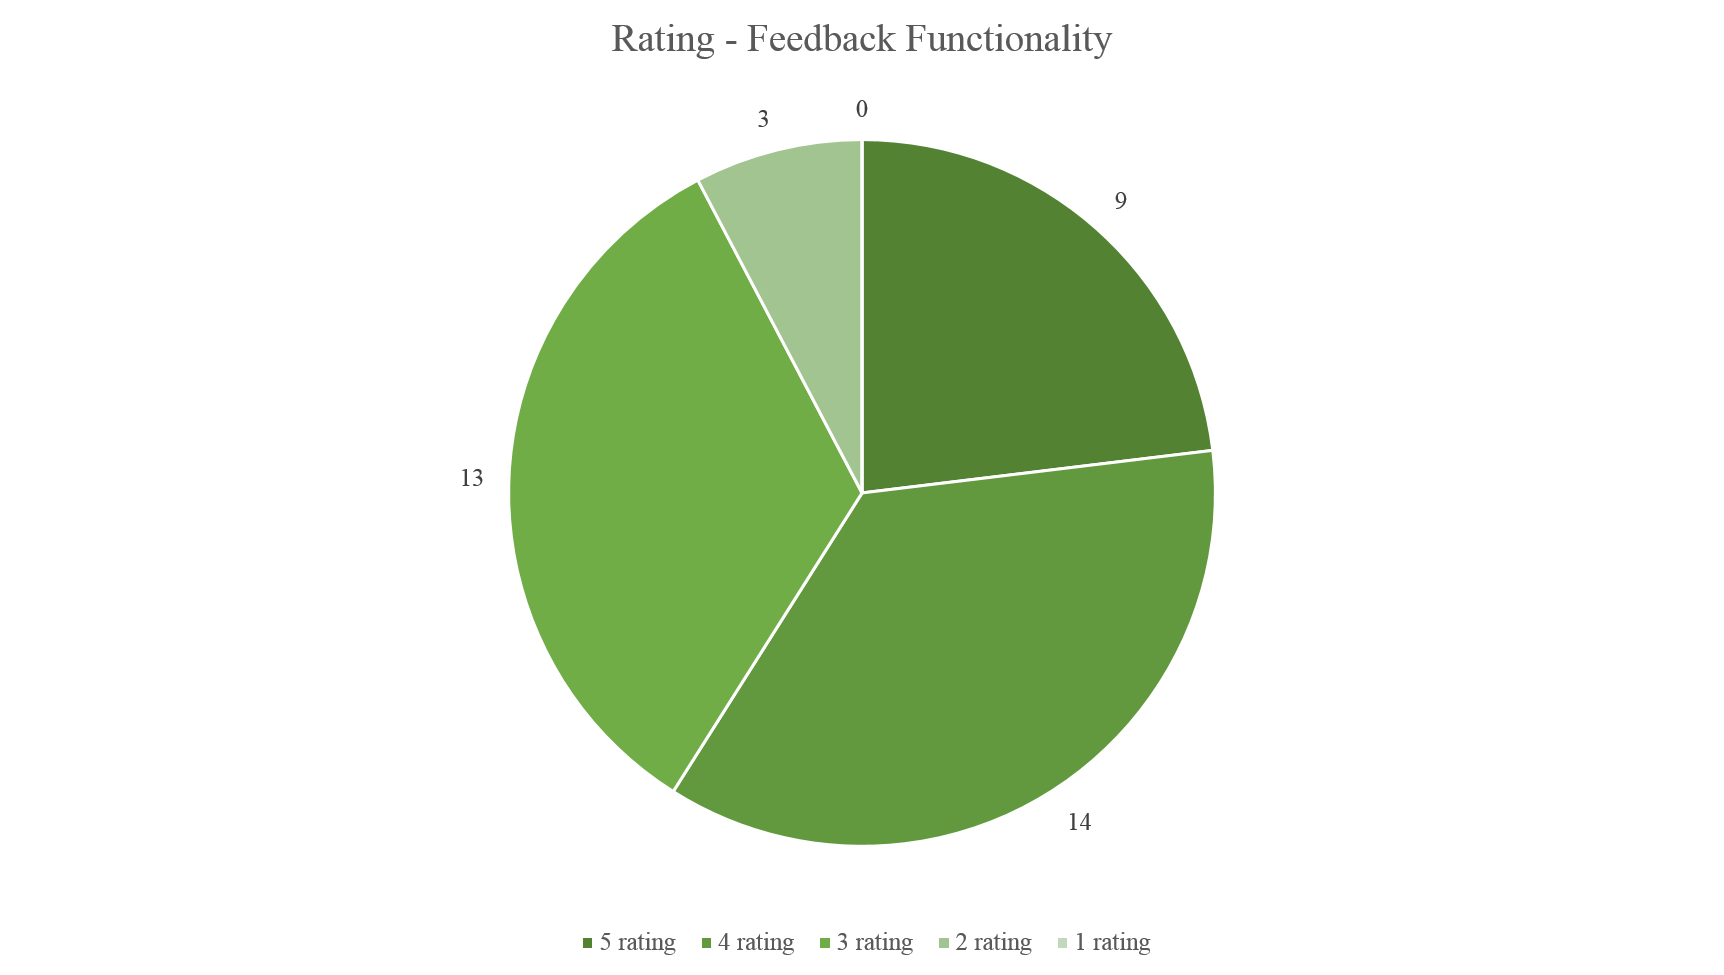
\includegraphics [scale=0.5] {ratingFeedbackFunctionality}
\caption [Chart - Rating - Feedback Functionality] {Chart - Rating - Feedback Functionality}
\label {image-ratingFeedbackFunctionality}
\end {figure}

\begin{table} [h]
\centering
\begin{tabular}{|l|c|}
\hline
Rating & Number of participants \\
\hline
5	&08 \\
4	&16 \\
3	&10 \\
2	&05 \\
1	&00 \\
\hline
\end{tabular}
\caption{Rating - Complaints Functionality}
\label{table-survey-rating-ComplaintsFunctionality}
\end{table}

\begin {figure} [h]
\centering
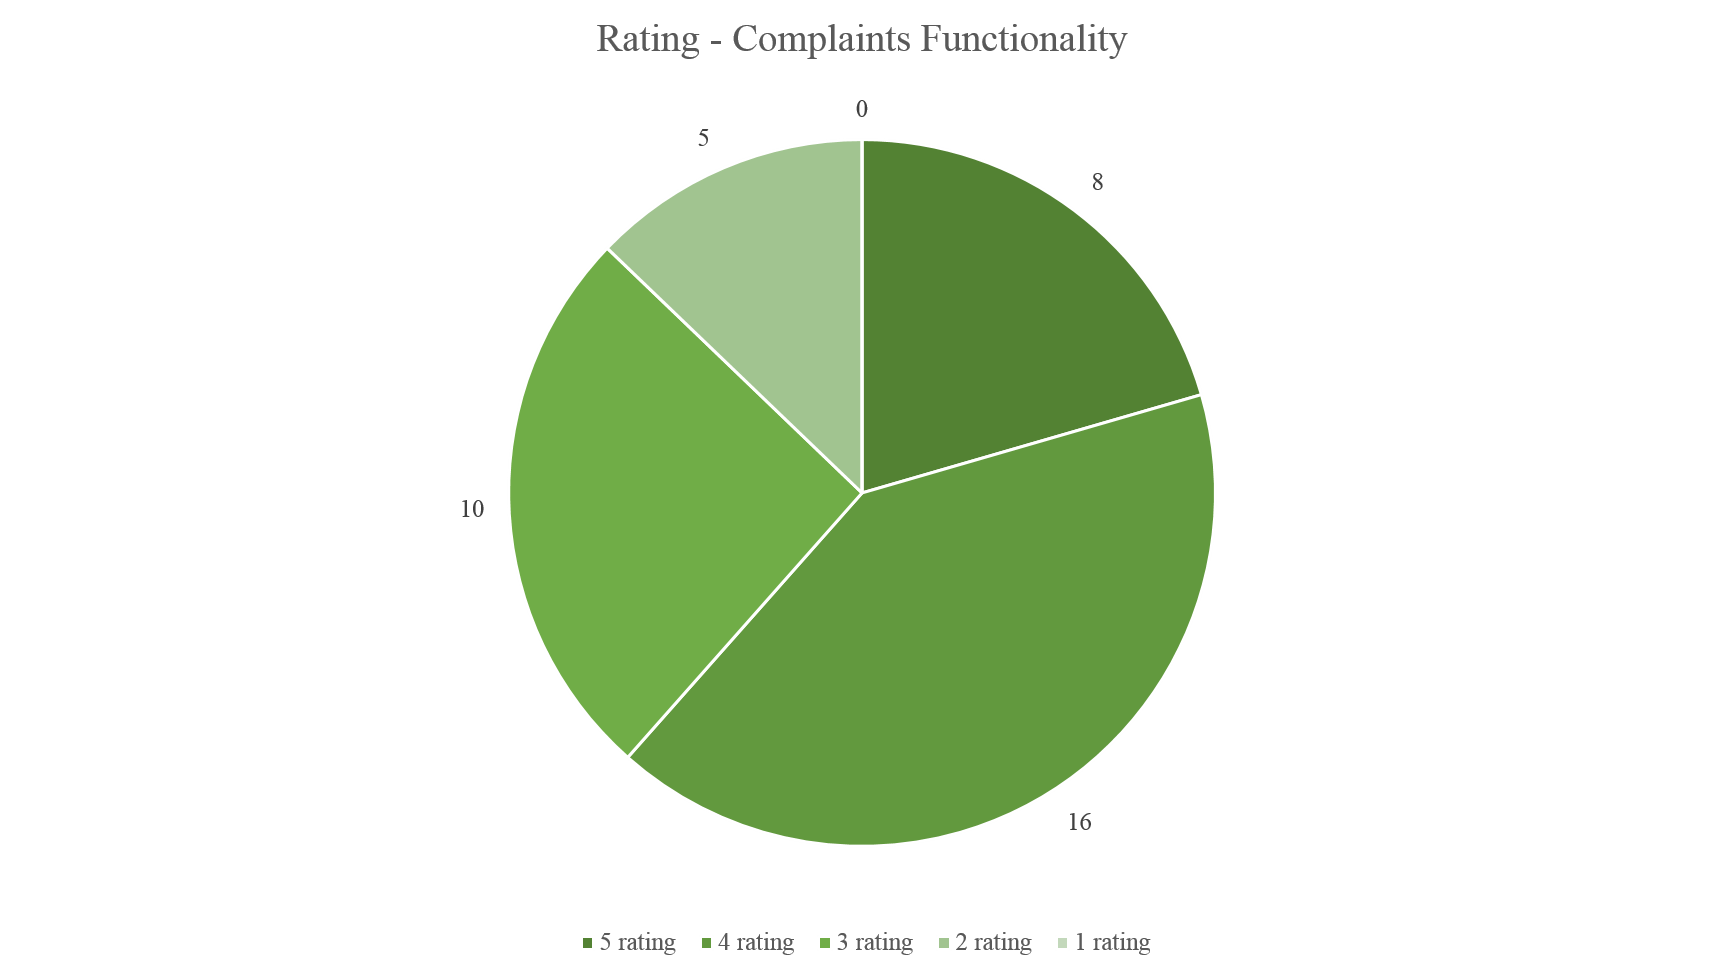
\includegraphics [scale=0.5] {ratingComplaintsFunctionality}
\caption [Chart - Rating - Complaints Functionality] {Chart - Rating - Complaints Functionality}
\label {image-ratingComplaintsFunctionality}
\end {figure}

\begin{table} [h]
\centering
\begin{tabular}{|l|c|}
\hline
Rating & Number of participants \\
\hline
5	&16 \\
4	&11 \\
3	&09 \\
2	&02 \\
1	&01 \\
\hline
\end{tabular}
\caption{Rating - User Interface}
\label{table-survey-rating-UserInterface}
\end{table}

\begin {figure} [h]
\centering
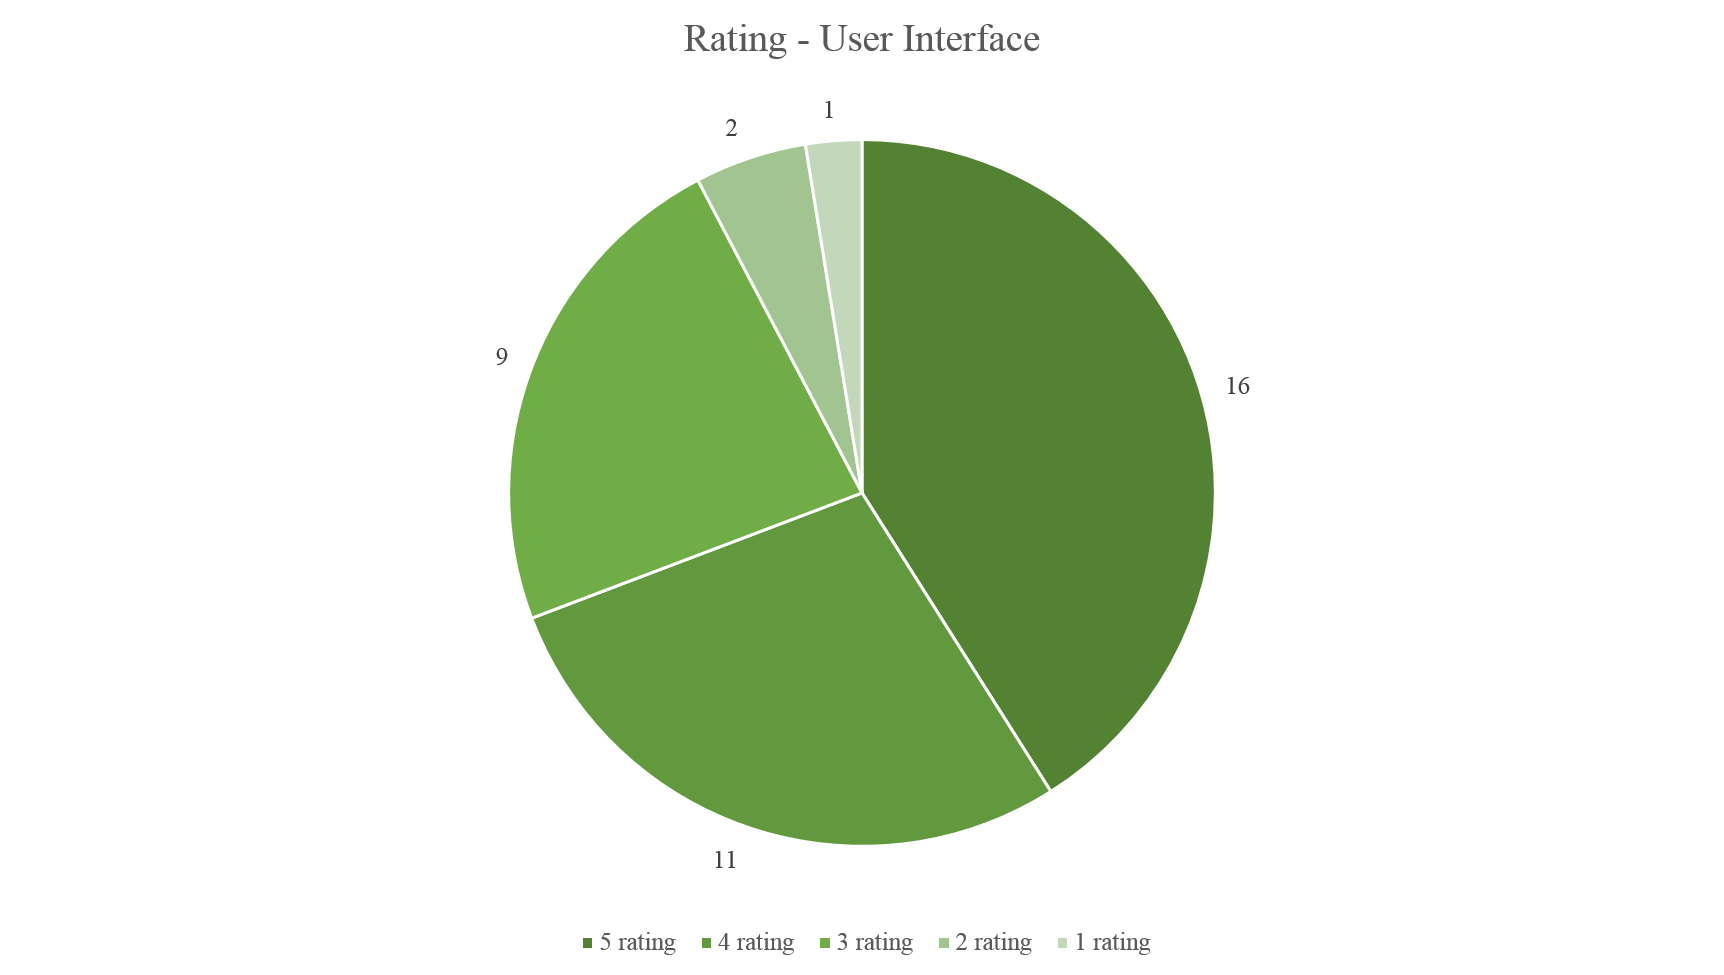
\includegraphics [scale=0.5] {ratingUserInterface}
\caption [Chart - Rating - User Interface] {Chart - Rating - User Interface}
\label {image-ratingUserInterface}
\end {figure}

\begin{table} [h]
\centering
\begin{tabular}{|l|c|}
\hline
Rating & Number of participants \\
\hline
Oh my god, yes!	&16 \\
Yes	&17 \\
No	&06 \\
\hline
\end{tabular}
\caption{Survey Question - Would you use a system like this if it was implemented?}
\label{table-survey-question-WouldYouUseASystemLikeThis}
\end{table}

\begin {figure} [h]
\centering
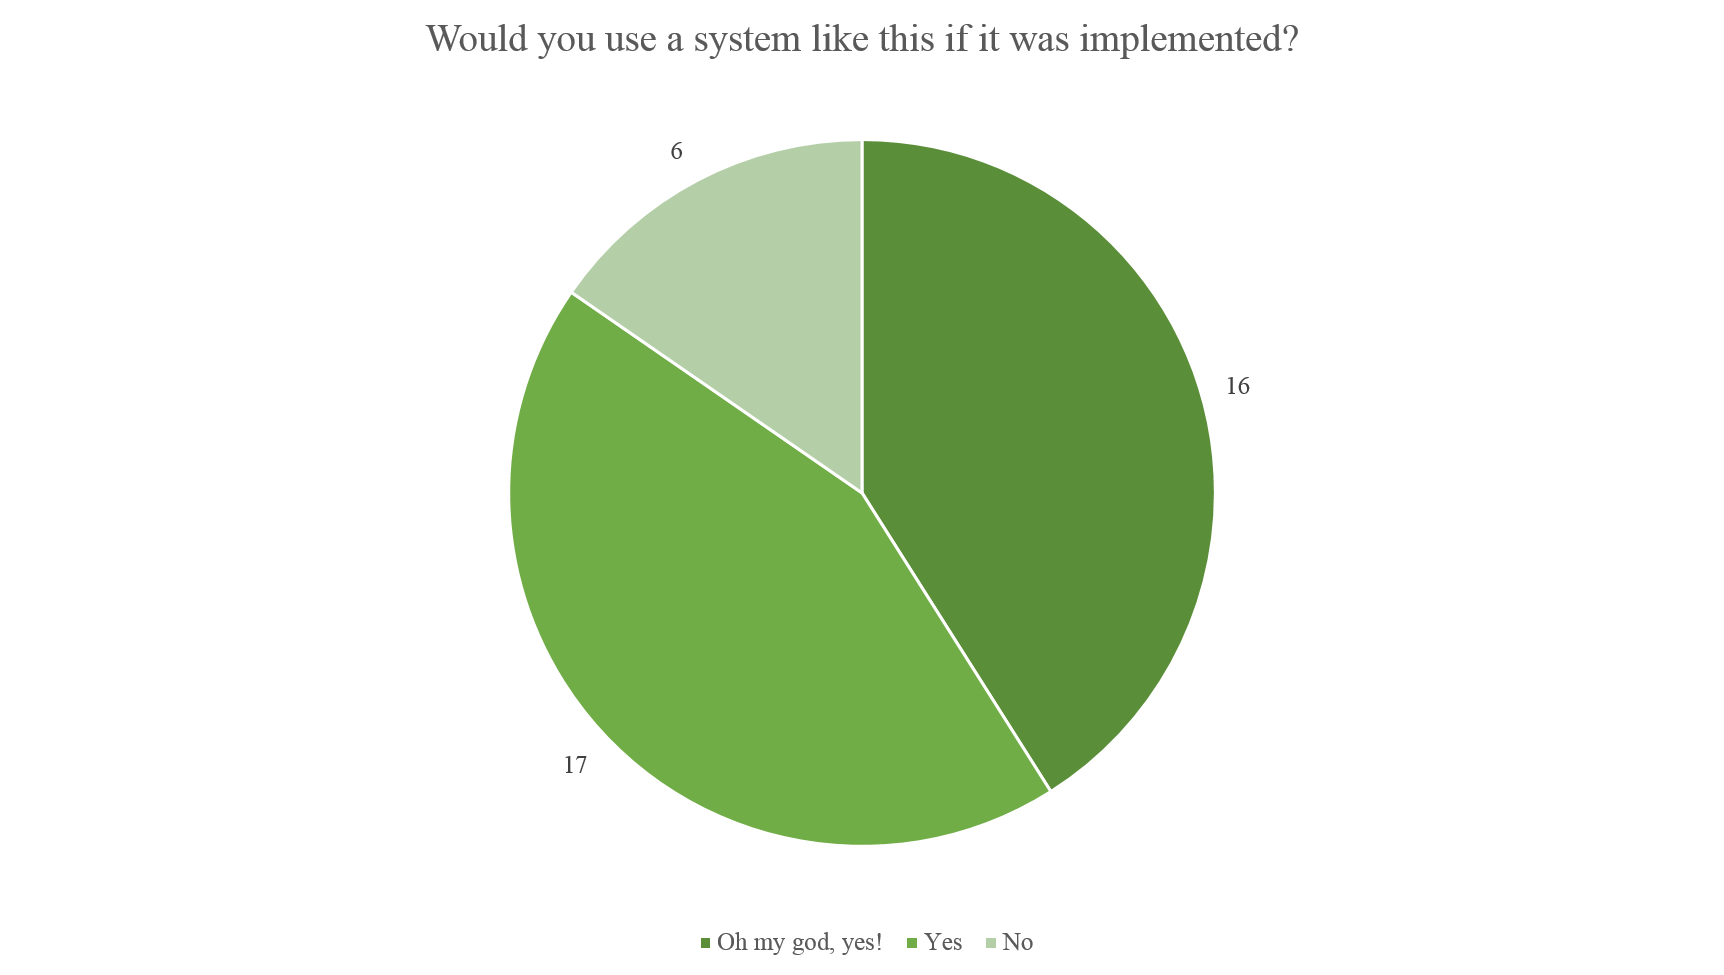
\includegraphics [scale=0.5] {questionWouldYouUse}
\caption [Chart - Survey Question] {Chart - Survey Question}
\label {image-questionWouldYouUse}
\end {figure}

\end {itemize}

\newpage

\section{Literature Published related to this Research Project}

\paragraph{} A research paper on the work related to this research project was submitted to the 2013 European, Mediterranean \& Middlle-eastern Conference on Information Systems (EMCIS). The paper was accepted subject to changes. The paper was an analysis of trasnportation systems in developing countries and how an Information Systems solution would help solve the problems faced in the public transportation domain. The details of the paper are listed below.

\begin {itemize}
\item Title: "A Transportation Management Information System for Public Transport in Developing Countries."
\item Authors: Jaldin, Aftha and Arunatileka, Dr. Shiromi.
\item Abstract: Public Transportation Management in developing countries presents a more challenging environment than its counterpart in developed nations. And, as in any Public Transport System, the Scheduling Process provides the framework in which the Transport Service operates. It is responsible for the formulation of timetables, vehicle and crew scheduling, and crew rostering. Although this is the most important part of the transport system, it is the most difficult to manage. The varied inputs to the process, the lack of proper infrastructure and improper technology and processes available all lead to a unique problem in terms of Public Transportation Management in a developing country. Therefore it is imperative for a system to cater to these limitations and meet the demands of a developing country specifically. Therefore, this paper proposes an alternative system to aid the Schedulers in their capacity to formulate timetables and schedule vehicles and crew. The system will also act as an information portal to commuters to obtain information about transport modes and associated routes as well as other related information. The paper uses the case of the Western Province Bus Transportation System in Sri Lanka as an example to draw conclusions regarding the proposed information system.
\end {itemize}

% begin Chapter ConclusionAndFutureWork

\chapter {Conclusion and Future Work}
\label{chapter-ConclusionAndFutureWork}

\section{Conclusion}
\label{section-Conclusion}

\paragraph{} This research project looked at the public transportation problem in developing countries like Sri Lanka. The research commenced with the intention of looking into the problems that the Western Province Private Bus Service was facing and possibly providing solutions for them. Over the course of the project, the service and the prevalent system was analyzed and the requirements were gathered. Consequently a hypothesis was formed regarding the usage of a Decision Support System to alleviate the issues. A prototype was then built with the intention of gaining further insight into the requirements of the users and the concept of using a decision support system in the context of public transportation.

The main outcome of this research project was to identify and analyze the problems in the public transportation system in the western province. Testing the concept of using a decision support system within this domain was also an important outcome of this project. We can now show that a DSS with a similar architecture and concept would work in other developing countries as well. The main point of applying this DSS concept is the cost benefit. As this is an open-source project, it is greatly beneficial for government entities such as the WP RPTA. Similarly, this same concept could be applied in other developing countries around the world.


\section{Future Work}
\label{section-FutureWork}

\paragraph{} The research of investigating the usage of a DSS in the context of a public transportation system in a developing country was in and of itself a challenge. Furthermore, this research can be extended in breadth to include an Automated Data Gathering Mechanism. The Data Collection framework and infrastructure was not within the scope of this research project. However, in the future, the methods of integrating a system of Automated Data Collection into this concept could be investigated. This includes an Automated Vehicle Location system as well as an Automated Passenger Counting mechanism. it could also investigate the possible options for an Automated Fare Collection framework and infrastructure. Possible options for the last point would be using mobile SMS-based payments and/or using new technologies such as NFC (Near-Field Communication) to implement a Contactless Smart Card system to reduce revenue leakage.

Additionally, the concept of the system presented in this research project could be extended to become an Expert System. An Expert System differs from a Decision Support System in that it not only provides the information to help the decision-making process but also provides several recommendations automatically by analyzing the data and identifying key points in the information. An Expert System is defined as a computer system that emulates the decision-making ability of a human expert. Expert systems are designed to solve complex problems by reasoning about knowledge, like an expert \cite{Jackson1998}.

This research project could also be extended by researching the various methods of bus dispatching and providing options for the schedulers to switch between various dispatching methods for each Bus Route or a set of Bus Routes.

The possible extensions to this research have been illustrated in Figure~\ref{image-futureWork}.

\begin {figure} [h]
\centering
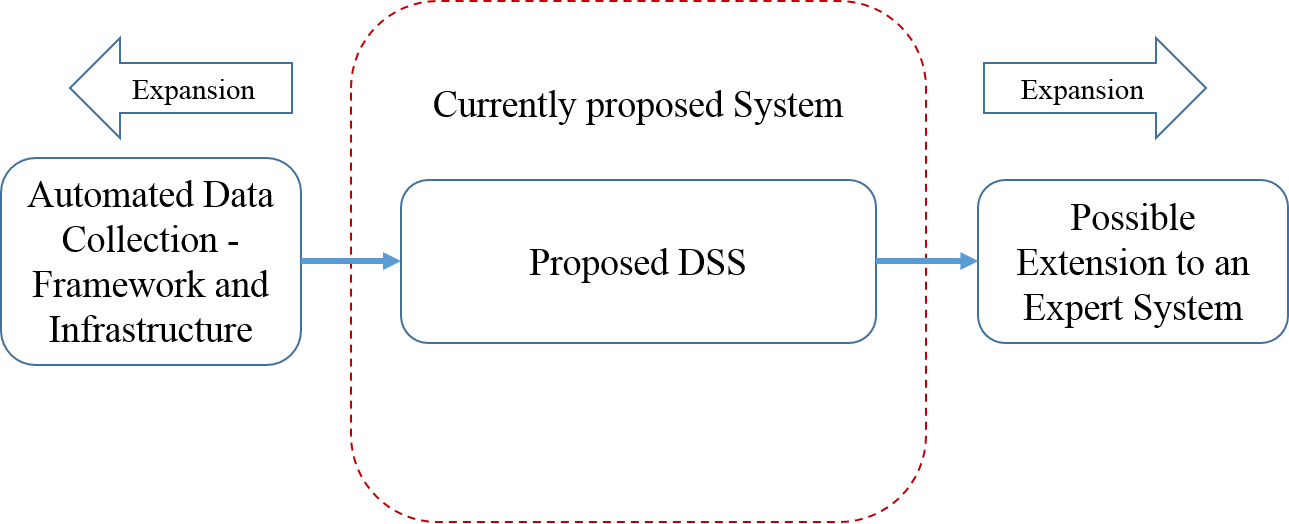
\includegraphics [scale=0.5] {futureWork}
\caption [Future Work and possible Expansion of Concept] {Future Work and possible Expansion of Concept}
\label {image-futureWork}
\end {figure}

\subsection{Localization to include Sinhala and Tamil Languages}

\paragraph{} Additionally, the system could be localized to improve usability by the Users. The DSS could be offered in Sinhala and Tamil languages so that people who have difficulty perusing the English web application could use the interface with the language that they are most comfortable with.

% begin Appendix

\appendix
\chapter{Complete Set of Gathered Data}
\label{appendix-CompleteSetOfData}

\paragraph{ } The fields that are highlighted in the tables are unauthorized stops at which the buses picked up or dropped off passengers.

\begin{enumerate}

\item Trip Number: 2
\begin{itemize}
\item Date: 23/5/2013
\item Departure Time: 17.00pm
\item Departure Place: Kolpetty
\item Table~\ref{table-trip2-BoardingAndAlighting} and~\ref{table-trip2-LoiterTime}
\end{itemize}

\item Trip Number: 3
\begin{itemize}
\item Date: 23/5/2013
\item Departure Time: 18.14pm
\item Departure Place: Kolpetty
\item Table~\ref{table-trip3-BoardingAndAlighting} and~\ref{table-trip3-LoiterTime}
\end{itemize}

\item Trip Number: 4
\begin{itemize}
\item Date: 23/5/2013
\item Departure Time: 16.28pm
\item Departure Place: Rajagiriya
\item Table~\ref{table-trip4-BoardingAndAlighting} and~\ref{table-trip4-LoiterTime}
\end{itemize}

\item Trip Number: 5
\begin{itemize}
\item Date: 23/5/2013
\item Departure Time: 17.43pm
\item Departure Place: Rajagiriya
\item Table~\ref{table-trip5-BoardingAndAlighting} and~\ref{table-trip5-LoiterTime}
\end{itemize}

\end{enumerate}

%data tables

\begin{table}
\centering
\begin{tabular}{|l|r|r|r|r|}
\hline
Bus Stop & Boarded & Alighted & Net Gain & On Board \\
\hline
 & & & & 0 \\
Kolpetty Depot	&21	&0	&21	&21\\
Supermarket	&7	&1	&6	&27\\
Alwis Place	&5	&0	&5	&32\\
\rowcolor[gray]{0.7}
Citibank	&2	&0	&2	&34\\
Library	&7	&2	&5	&39\\
SLTA	&0	&1	&-1	&38\\
Nelum Pokuna	&3	&0	&3	&41\\
\rowcolor[gray]{0.7}
Alexandra Roundabout	&3	&0	&3	&44\\
\rowcolor[gray]{0.7}
Saudi Embassy	&1	&0	&1	&45\\
Asha Central	&6	&0	&6	&51\\
Wijerama	&0	&0	&0	&51\\
Borella	&9	&2	&7	&58\\
Devi Balika	&5	&0	&5	&63\\
Castle Street	&0	&0	&0	&63\\
Ayurveda	&0	&9	&-9	&54\\
Rajagiriya	&11	&7	&4	&58\\
\hline
\end{tabular}
\caption{Boarding And Alighting data for Trip 2}
\label{table-trip2-BoardingAndAlighting}
\end{table}

\begin{table}
\centering
\begin{tabular}{|l|r|r|r|}
\hline
Bus Stop & Arrival Time (h) & Departure Time (h) & Loiter Time (mins) \\
\hline
Kolpetty Depot	&	&17.03	&0\\
Supermarket	&17.03	&17.04	&1\\
Alwis Place	&17.05	&17.05	&0\\
Library	&17.08	&17.08	&0\\
SLTA	&17.09	&17.09	&0\\
Nelum Pokuna	&17.11	&17.12	&1\\
Asha Central	&17.15	&17.16	&1\\
Wijerama	&17.17	&17.18	&1\\
Borella	&17.21	&17.25	&4\\
Devi Balika	&17.27	&17.27	&0\\
Castle Street	&17.29	&17.29	&0\\
Ayurveda	&17.31	&17.38	&7\\
Rajagiriya	&17.40	&17.43	&3\\
\hline
Total Loiter Time & & & 18 mins \\
Duration of Trip & & 40 mins & \\
\hline
\end{tabular}
\caption{Loiter Time Data for Trip 2}
\label{table-trip2-LoiterTime}
\end{table}

\begin{table}
\centering
\begin{tabular}{|l|r|r|r|r|}
\hline
Bus Stop & Boarded & Alighted & Net Gain & On Board \\
\hline
 & & & & 0 \\
Kolpetty Depot	&37	&0	&37	&37\\
Supermarket	&10	&0	&10	&47\\
Alwis Place	&1	&0	&1	&48\\
Library	&4	&3	&1	&49\\
SLTA	&1	&0	&1	&50\\
\rowcolor[gray]{0.7}
Museum	&2	&0	&2	&52\\
Nelum Pokuna	&5	&2	&3	&55\\
Saudi Embassy	&0	&0	&0	&55\\
Asha Central	&3	&1	&2	&57\\
Wijerama	&0	&0	&0	&57\\
Borella	&10	&6	&4	&61\\
Devi Balika	&1	&0	&1	&62\\
Castle Street	&6	&2	&4	&66\\
Ayurveda	&3	&5	&-2	&64\\
Rajagiriya	&18	&12	&6	&70\\
\hline
\end{tabular}
\caption{Boarding And Alighting data for Trip 3}
\label{table-trip3-BoardingAndAlighting}
\end{table}

\begin{table}
\centering
\begin{tabular}{|l|r|r|r|}
\hline
Bus Stop & Arrival Time (h) & Departure Time (h) & Loiter Time (mins) \\
\hline
Kolpetty Depot	&	&18.19	&0\\
Supermarket	&18.20	&18.22	&2\\
Alwis Place	&18.23	&18.24	&1\\
Library	&18.26	&18.26	&0\\
SLTA	&18.28	&18.28	&0\\
Nelum Pokuna	&18.30	&18.30	&0\\
Asha Central	&18.35	&18.35	&0\\
Wijerama	&18.35	&18.35	&0\\
Borella	&18.37	&18.38	&1\\
Devi Balika	&18.41	&18.41	&0\\
Castle Street	&18.43	&18.43	&0\\
Ayurveda	&18.45	&18.45	&0\\
Rajagiriya	&18.47	&18.53	&6\\
\hline
Total Loiter Time & & & 10 mins \\
Duration of Trip & & 34 mins & \\
\hline
\end{tabular}
\caption{Loiter Time Data for Trip 3}
\label{table-trip3-LoiterTime}
\end{table}

\begin{table}
\centering
\begin{tabular}{|l|r|r|r|r|}
\hline
Bus Stop & Boarded & Alighted & Net Gain & On Board \\
\hline
 & & & & 19 \\
Rajagiriya	&15	&1	&14	&33\\
Cotta Road	&2	&0	&2	&35\\
Ayurveda	&4	&3	&1	&36\\
Castle Street	&3	&1	&2	&38\\
Borella	&2	&3	&-1	&37\\
Horton Place	&2	&2	&0	&37\\
Wijerama	&0	&2	&-2	&35\\
Asha Central	&7	&0	&7	&42\\
Nelum Pokuna	&2	&4	&-2	&40\\
Library	&19	&0	&19	&59\\
Liberty	&2	&16	&-14	&45\\
Galle Road	&0	&1	&-1	&44\\
\rowcolor[gray]{0.7}
St. Anthony's Mw	&1	&2	&-1	&43\\
Kolpetty Depot	&0	&43	&-43	&0\\
\hline
\end{tabular}
\caption{Boarding And Alighting data for Trip 4}
\label{table-trip4-BoardingAndAlighting}
\end{table}

\begin{table}
\centering
\begin{tabular}{|l|r|r|r|}
\hline
Bus Stop & Arrival Time (h) & Departure Time (h) & Loiter Time (mins) \\
\hline
Rajagiriya	&16.28	&16.33	&5\\
Cotta road	&16.34	&16.34	&0\\
Ayurveda	&16.35	&16.36	&1\\
Castle street	&16.38	&16.39	&1\\
Borella	&16.40	&16.41	&1\\
Horton Place	&16.42	&16.42	&0\\
Wijerama	&16.44	&16.44	&0\\
Asha Central	&16.47	&16.47	&0\\
Nelum Pokuna	&16.48	&16.48	&0\\
Library	&16.50	&16.50	&0\\
Liberty	&16.52	&16.52	&0\\
Galle Road	&16.54	&16.54	&0\\
Kolpetty Depot	&16.55	&	&0\\
\hline
Total Loiter Time & & & 8 mins \\
Duration of Trip & & 22 mins & \\
\hline
\end{tabular}
\caption{Loiter Time Data for Trip 4}
\label{table-trip4-LoiterTime}
\end{table}

\begin{table}
\centering
\begin{tabular}{|l|r|r|r|r|}
\hline
Bus Stop & Boarded & Alighted & Net Gain & On Board \\
\hline
 & & & & 30 \\
Rajagiriya	&5	&2	&3	&33\\
Cotta Road	&2	&0	&2	&35\\
Ayurveda	&0	&4	&-4	&31\\
Castle Street	&2	&0	&2	&33\\
Borella	&1	&6	&-5	&28\\
Horton Place	&3	&2	&1	&29\\
\rowcolor[gray]{0.7}
Chatz	&1	&0	&1	&30\\
Wijerama	&1	&0	&1	&31\\
Asha Central	&1	&1	&0	&31\\
Nelum Pokuna	&5	&3	&2	&33\\
Library	&4	&3	&1	&34\\
Liberty	&0	&8	&-8	&26\\
Galle Road	&0	&4	&-4	&22\\
\rowcolor[gray]{0.7}
St. Anthony's Mw	&4	&3	&1	&23\\
Kolpetty Depot	&0	&23	&-23	&0\\
\hline
\end{tabular}
\caption{Boarding And Alighting data for Trip 5}
\label{table-trip5-BoardingAndAlighting}
\end{table}

\begin{table}
\centering
\begin{tabular}{|l|r|r|r|}
\hline
Bus Stop & Arrival Time (h) & Departure Time (h) & Loiter Time (mins) \\
\hline
Rajagiriya	&17.40	&17.43	&3\\
Cotta Road	&17.44	&17.45	&1\\
Ayurveda	&17.49	&17.49	&0\\
Castle Street	&17.52	&17.52	&0\\
Borella	&17.55	&17.56	&1\\
Horton Place	&17.57	&17.58	&1\\
Wijerama	&17.59	&17.59	&0\\
Asha Central	&18.00	&18.00	&0\\
Nelum Pokuna	&18.01	&18.02	&1\\
Library	&18.03	&18.03	&0\\
Liberty	&18.05	&18.05	&0\\
Galle Road	&18.08	&18.08	&0\\
Kolpetty Depot	&18.09	&	&0\\
\hline
Total Loiter Time & & & 7 mins \\
Duration of Trip & & 26 mins & \\
\hline
\end{tabular}
\caption{Loiter Time Data for Trip 5}
\label{table-trip5-LoiterTime}
\end{table}


\backmatter
\bibliographystyle{plain}
\bibliography{FYP}

\end{document}  